\documentclass[conference]{IEEEtran}
\pagestyle{plain}


\usepackage{times}
\usepackage[utf8]{inputenc}
\usepackage{url}
\usepackage{amssymb}
\usepackage{amsmath}
\usepackage{array,multirow}
\usepackage{xspace}
\usepackage{xcolor}
\usepackage{color, colortbl} 
\usepackage{balance}
\usepackage{paralist}
\usepackage{hyperref}
\usepackage{cleveref}
\usepackage{graphicx}
\usepackage{pifont}
\usepackage{array}
\usepackage{booktabs}
\usepackage{tikz}
\usepackage{bm}
%\usepackage{enumitem}%not compatible with IEEEtran it seems
\setlength {\marginparwidth}{2cm}
\usepackage{todonotes}
\usepackage{arydshln}
\usepackage{makecell}
\usepackage{tabularx}
\usepackage{authblk}
\usepackage{caption}
\usepackage{soul,color}
%\usepackage{subcaption}
\usepackage{mwe}
\usepackage{ifthen}
\usepackage{algorithm}
\usepackage[noend]{algpseudocode}
\usepackage{epsfig}
\usepackage[tight,footnotesize]{subfigure}

\newcommand{\cmark}{\ding{51}}%
\newcommand{\xmark}{\ding{55}}%

%!TEX root = main.tex
%=========================================================

% use true/false to toggle all comments (both kinds)

\newboolean{showcomments}
\setboolean{showcomments}{false}

% ====== comments ======
\newcommand\important[1]{\todo[inline]{\textbf{Important:} #1}}
\newcommand\alberto[1]{\todo[color=yellow,inline]{\textbf{Alberto:} #1}}
\newcommand\etienne[1]{\todo[color=orange,inline]{\textbf{Etienne:} #1}}
\newcommand\pierre[1]{\todo[color=brown,inline]{\textbf{Pierre:} #1}}
\newcommand\felix[1]{\todo[color=blue!40,inline]{\textbf{Felix:} #1}}
\newcommand\michal[1]{\todo[color=green,inline]{\textbf{Michał:} #1}}
\newcommand\onur[1]{\todo[color=red,inline]{\textbf{Onur:} #1}}
\newcommand\sergi[1]{\todo[color=pink,inline]{\textbf{Sergi:} #1}}
\newcommand\ramin[1]{\todo[color=brown,inline]{\textbf{Ramin:} #1}}
\newcommand\mustafa[1]{\todo[color=brown,inline]{\textbf{Mustafa:} #1}}
% Uncomment the following command to make all comments disappear
\ifthenelse{\boolean{showcomments}} { }
{
\renewcommand\important[1]{}
\renewcommand\alberto[1]{}
\renewcommand\mustafa[1]{}
\renewcommand\michal[1]{}
\renewcommand\onur[1]{}
\renewcommand\sergi[1]{}
\renewcommand\etienne[1]{}
\renewcommand\pierre[1]{}
\renewcommand\ramin[1]{}
\renewcommand\felix[1]{}
}

% ====== inlined and toggable comments ======

\ifthenelse{\boolean{showcomments}}
{ \newcommand{\mynote}[3]{
    \protect\fbox{\bfseries\sffamily\scriptsize#1}
    {\small\textsf{\emph{\color{#3}{#2}}}}}}
{ \newcommand{\mynote}[3]{}}

\newcommand{\er}[1]{\mynote{Etienne}{#1}{blue}}
\newcommand{\mk}[1]{\mynote{Michał}{#1}{brown}}
\newcommand{\sr}[1]{\mynote{Sergi}{#1}{red}}

% \newcommand{\xxx}[1]{\mynote{YourName}{#1}{black!20!red!80!}}
% \newcommand{\xxx}[1]{\mynote{YourName}{#1}{green}}
\newcommand{\as}[1]{\mynote{Alberto}{#1}{orange}}
\newcommand{\dk}[1]{\mynote{Daniel}{#1}{green}}
\newcommand{\rs}[1]{\mynote{Ramin}{#1}{violet}}
\newcommand{\oa}[1]{\mynote{Onur}{#1}{red}}

% ====== systems ======
% \newcommand\sysname{TOPDISC\xspace}
\newcommand\sysname{DISCv5\xspace}
\newcommand\discv{DISCv4\xspace}
\newcommand\altname{DHT\xspace}
\newcommand\altnameticket{DHTTicket\xspace}
\newcommand\altsysname{PMETIS\xspace}
\newcommand\sysnamePriv{Pineapple\xspace}
\newcommand\sysnameAnon{\coconut}
\newcommand\libcoin{LibraCoin\xspace}
\newcommand\libcoins{LibraCoins\xspace}
\newcommand\privcoin{PrivCoin\xspace}
\newcommand\privcoins{PrivCoins\xspace}

\newcommand\sysnamereplay{\texttt{byzcuit}\xspace}
\newcommand\sysnamebaseline{\texttt{byzcuit-baseline}\xspace}
\newcommand\simplesysname{Simple-\sysname}

\newcommand\libra{Libra\xspace}
\newcommand\fourier{Fourier\xspace}
\newcommand\chainspace{Chainspace\xspace}
\newcommand\ethereum{Ethereum\xspace}
\newcommand\hyperledger{Hyperledger\xspace}
\newcommand\omniledger{Omniledger\xspace}
\newcommand\rapidchain{RapidChain\xspace}
\newcommand\elgamal{El-Gamal\xspace}
\newcommand\coconut{Coconut\xspace}
\newcommand\macggm{$\bm{\mathrm{MAC_{GGM}}}$\xspace}
\newcommand\sbac{S-BAC\xspace}
\newcommand\bft{BFT\xspace}
\newcommand\atomix{Atomix\xspace}
\newcommand\cscoin{CSCoin\xspace}
\newcommand\rscoin{RSCoin\xspace}
\newcommand\lsbac{\sysname}
\newcommand\fsbac{F-SBAC\xspace}
\newcommand\bftsmart{\textsc{bft-SMaRt}\xspace}

\makeatletter
\def\BState{\State\hskip-\ALG@thistlm}
\makeatother

% ====== custom notations ======
%\newcommand\algorithm[1]{\textsf{#1}}
\newcommand\hashtopoint{H^*\xspace}
\newcommand\stringtopoint{H'\xspace}
\newcommand\function[1]{\ding{118}\xspace \textsf{#1}:\xspace}
\newcommand\shard[1]{\emph{shard}\xspace#1\xspace}
\newcommand\Shard[1]{\emph{Shard}\xspace#1\xspace}
\newcommand\preacceptt{\textsf{pre-accept}($T$)\xspace}
\newcommand\preabortt{\textsf{pre-abort}($T$)\xspace}
\newcommand\preaccepttt{\textsf{pre-accept}($T'$)\xspace}
\newcommand\preaborttt{\textsf{pre-abort}($T'$)\xspace}
\newcommand\preacceptttt{\textsf{pre-accept}($T''$)\xspace}
\newcommand\preacceptts{\textsf{pre-accept}($T,s_T$)\xspace}
\newcommand\preabortts{\textsf{pre-abort}($T,s_T$)\xspace}
\newcommand\preabortttt{\textsf{pre-abort}($T''$)\xspace}
\newcommand\acceptt{\textsf{accept}($T$)\xspace}
\newcommand\abortt{\textsf{abort}($T$)\xspace}
\newcommand\accepttt{\textsf{accept}($T'$)\xspace}
\newcommand\aborttt{\textsf{abort}($T'$)\xspace}
\newcommand\acceptttt{\textsf{accept}($T''$)\xspace}
\newcommand\abortttt{\textsf{abort}($T''$)\xspace}
\newcommand\acceptts{\textsf{accept}($T,s_T$)\xspace}
\newcommand\abortts{\textsf{abort}($T,s_T$)\xspace}
\newcommand\myrow[1]{row\xspace\textsf{#1}\xspace}
\newcommand\mycolumn[1]{column\xspace\textsf{#1}\xspace}
\newcommand\shardled{shard-led\xspace}
\newcommand\Shardled{Shard-led\xspace}
\newcommand\clientled{client-led\xspace}
\newcommand\Clientled{Client-led\xspace}
\newcommand\activeObj{`active'\xspace}
\newcommand\inactiveObj{`inactive'\xspace}
\newcommand\locked{`locked'\xspace}
\newcommand\wa{{WA}\xspace}
\newcommand\wb{{WB}\xspace}
\newcommand\ka{{KA}\xspace}
\newcommand\kb{{KB}\xspace}

% ====== concepts/terminology =======

\newcommand\attacker{attacker\xspace}
\newcommand\adversary{attacker\xspace}
\newcommand\prerecorded{prerecorded\xspace}
\newcommand\prerecords{prerecords\xspace}
\newcommand\prerecord{prerecord\xspace}

%  ===== formatting ======
% Abbreviations etc.
\newcommand{\cf}{cf.\@\xspace}
\newcommand{\vs}{vs.\@\xspace}
\newcommand{\etc}{etc.\@\xspace}
\newcommand{\ala}{ala\@\xspace}
\newcommand{\wrt}{w.r.t.\@\xspace}
\newcommand{\etal}{\textit{et al.}\@\xspace}
\newcommand{\eg}{\textit{e.g.}\@\xspace}
\newcommand{\Eg}{\textit{E.g.}\@\xspace}
\newcommand{\ie}{\textit{i.e.}\@\xspace}
\newcommand{\Ie}{\textit{I.e.}\@\xspace}
\newcommand{\via}{\textit{via}\@\xspace}
\newcommand{\defacto}{\textit{de facto}\@\xspace}

\newcommand\mypara[1]{\vspace{0.05in} \noindent \textbf{#1.}}
\newcommand\para[1]{\vspace{0.05in} \noindent \textbf{#1.}}


\newcommand\definition[2]{\ding{118}\xspace \textsf{#1}\xspace$\bm{\rightarrow}$\xspace(#2):\xspace}



% For inlined section titles.
\newcommand\inlinesection[1]{{\bf #1.}}

\def\first{({\it i})\xspace}
\def\second{({\it ii})\xspace}
\def\third{({\it iii})\xspace}
\def\fourth{({\it iv})\xspace}
\def\fifth{({\it v})\xspace}
\def\sixth{({\it vi})\xspace}

\newcommand{\one}{({\em i})\xspace}
\newcommand{\two}{({\em ii})\xspace}
\newcommand{\three}{({\em iii})\xspace}
\newcommand{\four}{({\em iv})\xspace}
\newcommand{\five}{({\em v})\xspace}

% Colours
\definecolor{verylightgray}{gray}{0.8}

% Table
\newcolumntype{L}{l<{\hspace{1cm}}}
\newcolumntype{C}{c<{\hspace{1cm}}}
\newcolumntype{D}{c<{\hspace{0.3cm}}}

% Markers
\newcommand\vgap{\vskip 2ex}
\newcommand\marker{\vgap\ding{118}\xspace}

\def\na{--}
\def\unsure{?}
\def\missing{$!$}
\newcommand{\yes}{\ding{51}}
\newcommand{\no}{\ding{55}}
\DeclareRobustCommand\pie[1]{
\tikz[every node/.style={inner sep=0,outer sep=0, scale=1.5}]{
\node[minimum size=1.5ex] at (0,-1.5ex) {}; 
 \draw[fill=white] (0,-1.5ex) circle (0.75ex); \draw[fill=black] (0.75ex,-1.5ex) arc (0:#1:0.75ex); 
}
}
\def\L{\pie{0}} % Low
\def\M{\pie{-180}} % Medium
\def\H{\pie{360}} % High


\begin{document}

\title{Topic-based service discovery for the Ethereum P2P network}
\title{\sysname: Robust, efficient, and decentralized service discovery for the Ethereum platform}
\author{}
\maketitle

\begin{abstract}
  Lorem ipsum dolor sit amet, consectetur adipisicing elit, sed do eiusmod tempor incididunt ut labore et dolore magna aliqua. Ut enim ad minim veniam, quis nostrud exercitation ullamco laboris nisi ut aliquip ex ea commodo consequat. Duis aute irure dolor in reprehenderit in voluptate velit esse cillum dolore eu fugiat nulla pariatur. Excepteur sint occaecat cupidatat non proident, sunt in culpa qui officia deserunt mollit anim id est laborum. Lorem ipsum dolor sit amet, consectetur adipisicing elit, sed do eiusmod tempor incididunt ut labore et dolore magna aliqua.
  
  Lorem ipsum dolor sit amet, consectetur adipisicing elit, sed do eiusmod tempor incididunt ut labore et dolore magna aliqua. Ut enim ad minim veniam, quis nostrud exercitation ullamco laboris nisi ut aliquip ex ea commodo consequat. Duis aute irure dolor in reprehenderit in voluptate velit esse cillum dolore eu fugiat nulla pariatur. Excepteur sint occaecat cupidatat non proident, sunt in culpa qui officia deserunt mollit anim id est laborum.
  
  
%   \er{needs a full rewrite}
% Peer-to-Peer (P2P) Networks  are being increasingly deployed in distributed systems. They are being used in blockchains (Ethereum, Bitcoin), storage systems (IPFS, Stor4j) and more. One of the main functionalities of P2P networks is the ability to collectively keep information in the form of a key-value store. However, the current implementations either trade security for efficiency (structured P2P networks) or vice-versa (unstructured P2P networks).
%
% In this work, we propose \sysname - a P2P key/value store implementation which enables secure, efficient and robust information storage and retrieval. Our system can be deployed on any Distributed Hash Table (DHT). \sysname stores data on multiple nodes for increased security and allows discovering that data within a bounded amount of time guaranteeing high efficiency. We implement a robust admission mechanism limiting the resource usage by its participants and preventing a vast range of malicious behaviours.
%
% We present the design of \sysname and evaluate the system in multiple scenarios. Compared to the state-of-the-art, our system achieves high security, more equal load distribution, lower computational and communication overhead and better robustness in the presence of a powerful attacker.

%The Ethereum blockchain runs a Peer-to-Peer (P2P) network that rely on Kademlia Distributed Hash Table (DHT) for peer discovery and exchanging pending transactions and mined blocks. 
%Apart from supporting blockchain data exchange, the Ethereum P2P network is used by other applications taking advantage of the existing infrastructure to facilitate bootstraping of their own, application-specific networks. However, in order to achieve this task, peers using the same application must first find each other among other, unrelated nodes.

%In this work, we propose a service discovery system (\sysname) which enables secure and robust discovery of application-specific peers in a large, host P2P network. 
%Our system enables nodes to associate themselves with a set of \emph{topics}. The association is collectively stored by the network, and can be later found by interested peers within a bounded amount of time. \sysname included a robust admission mechanism limiting the resource usage by its participants and preventing a vast range of malicious behaviours. 
\end{abstract}


%%!TEX root = ../main.tex
%=========================================================

\section{Introduction}
\para{Motivation} Ethereum~\cite{buterin2013ethereum}  is one of the largest permissionless,  open-source  blockchains supporting Turing-complete scripting via smart contracts. Ethereum runs a Peer-to-Peer (P2P) network based on Kademlia Distributed Hash Table (DHT) ~\cite{maymounkov2002kademlia} to exchange pending transactions and mined blocks. 

%Following its decentralized design, Ethereum relies on a Peer-to-Peer (P2P) communication network, where individual nodes, running an Ethereum client software (\eg Go Ethereum~\cite{go-ethereum}), send and receive messages containing transactions and blocks to achieve distributed consensus, without relying on any central node or a trusted third party. The core system and the associated protocols used by the peers to participate in the Ethereum P2P network is included as part of a suite called DEVp2p. The suite includes individual sub-systems and protocols for services such as node discovery or establishing secure or point-to-point communication between peers. 

Apart from supporting blockchain data exchange, the Ethereum P2P network is also used by other applications. This includes multiple Ethereum testnets (Ropsten, Rinkeby),  alternative cryptocurrencies(Pirl, Musicoin) and other decentralized platforms such as iExec or Swarm.
In 2018, the Ethereum P2P network nodes operated a total of 4,076 different applications\cite{kim2018measuring}. Most of those applications require a dedicated P2P network to disseminate application-specific messages (\eg event notifications) to the interested peers but rely on the larger, Ethereum P2P network for bootstrapping.

Using an existing, well-established P2P network to bootstrap smaller, application specific networks has multiple advantages. Firstly, it encourages re-using reliable code to perform common tasks such as securing connections or finding peers. Secondly, P2P network security increases with the number of its honest participants. Being part of a larger swarm makes smaller applications more resistant to various attacks\hl{some refs from attack of smaller blockchains}. Finally, application developers can focus uniquely on implementing application-specific services boosting the growth of the entire, decentralised ecosystem. 

To realise this vision, nodes must \textit{(i)} join a larger, host P2P network, \textit{(ii)} discover their application-specific peers, \textit{(iii)} form an application-specific network. However, peer discovery in a fully decentralised setup is a challenging task. Unlike existing discovery protocols that work in a local setting (MDNS/Bonjour\hl{[?]}) or rely on trusted operators \hl{[?]}, decentralised node discovery must work at a global scale and in a fully decentralised setting. Due to the high heterogeneity of applications and (potentially constraint) peers, such a protocol must be efficient and introduce low communication and computational overhead. Finally, an open system, must protect against malicious actors trying to disturb network services, exhaust resources of honest peers or hijack application-specific networks. 

\para{State of the art} In the current Ethereum service discovery system, \ie discovery version 4 (Discv4), nodes perform a \textit{brute-force} discovery process. A node willing to discover application-specific peers randomly traverses the DHT and initiates connections with all the encountered nodes. A permanent connection is established only if a peer supports the same application and terminated otherwise. Such an approach provides strong security guarantees but results in a large communication overhead and long discovery times, particularly for unpopular applications with a small number of peers. While multiple, alternative discovery systems have been proposed \hl{[?]}, they rely on unrealistic assumptions \hl{[?]}, introduce high overhead or fail to operate in a presence of an adversary \hl{[?]}. 

\para{Discv5} In this work, we propose a new \textbf{service discovery sub-system} which enables secure,  efficient and robust  discovery of application-specific peers in the Ethereum network,  that will be part of the new DEVp2p  discovery system version 5 (\textit{\sysname}).
Different from Discv4, \sysname allows nodes (\ie advertisers) to associate themselves with a set of \emph{topics} (\eg application IDs), and advertise the association (\ie an ad) to the network. The information is collectively stored by network participants (\ie registrars) without relying on a single trusted party at any point. Any node can then query the network for a topic to obtain a list of application-specific peers and directly connect to them without disturbing other members of the network. 

We build \sysname on top of the existing Ethereum DHT to avoid major changes to the system and take advantage of the already existing routing infrastructure. The protocol propagates application-specific advertisements to multiple nodes chosen in an unpredictable way to protect against targeted attacks. Our design encourages diversity of advertisements stored at each registrar making the system resistant to network dynamics. At the same time, \sysname provides efficient peer discovery operations terminating within a bounded number of steps for all the topics regardless of their popularity. The protocol implements a robust admission mechanism to limit the resource usage on all the nodes, ensure fairness across topics, and prevent a vast range of malicious behaviours even in the presence of a powerful attacker.

\para{Contributions} We make the following contributions:
\begin{itemize}
    \item In \Cref{sec:placement}, we design a DHT-based data placement system that distributes service advertisement in the network. The protocol combines pseudo-random data placement for security with deterministic operations for efficiency. We present a lookup operation that finds a subset of advertisement placed in the system within a bounded amount of time. The procedure ensure the diversity of data sources and is resistant against manipulation by malicious registrars. 
    \item In \Cref{sec:registration} we design a lightweight admission protocol allowing advertisers to place ads after waiting for a specified amount of time. \sysname guarantees that advertisers cannot place more advertisement by deviating from the protocol and does not create any intermediary state at nodes holding the advertisements. 
    \item In \Cref{sec:waitingTime}, we design a function that calculates a waiting time after which advertisement can be placed on nodes holding advertisements. The function limits the amount of resources used by each node, promotes ads diversity stored within nodes, and protects against a vast range of malicious behaviours. 
\end{itemize}

In \Cref{sec:eval}, we evaluate \sysname under different system parameters and against state-of-the-art decentralised discovery systems. Our system achieves better load-balancing and requires more resource consumption by the attackers to successfully launch attacks such as eclipsing attacks. We also provide performance evaluation results from both simulations and from real system deployment. \sysname is scheduled for implementation in the next version of the Ethereum P2P network. 

%\michal{From the paragraph below we should form a requirements parts}
% An open and decentralized discovery system introduces new security challenges that need to be addressed. Malicious nodes may decide to deviate from the protocol in order to increase their own visibility or disrupt system operations. A particularly important security challenge is the \textit{Sybil attack} which can amplify the attacking power of malicious nodes, typically with very little resource consumption. The Sybils can launch various attacks including Denial-of-Service (DoS) by ignoring ad lookups, spam ads with bogus topic advertisement, and launch more sophisticated attacks to isolate nodes from their peers in their target sub-networks (\ie eclipse attack). 
%\michal{The above needs completion}
%\ramin{Is the above information about attacks needed in the introduction?}
%\michal{Probably not. We must just say there are problems with security}





% \er{Suggestions for alternative titles:
% \begin{itemize}
%   \item \sysname: Robust and efficient topic discovery in the Ethereum ecosystem
%   \item \sysname: Robust and efficient topic discovery in Ethereum 2.0
%   \item \sysname: Scalable and resilient topic membership management in Ethereum 2.0
%   \item \sysname: A robust and scalable topic discovery protocol for the next Ethereum generation
%   \item Resilient topic discovery in Ethereum with \sysname
%   \item Scalable and resilient topic discovery in Ethereum with \sysname
%   \item \sysname: Efficient, decentralized topic discovery for the Ethereum P2P network
%   \item \sysname: Robust and efficient decentralized membership management for applications of the Ethereum ecosystem
% \end{itemize}
% }

% %!TEX root = ../main.tex
%=========================================================

\er{General comments (20220914) after NDSS reject:
\begin{itemize}
	\item We need to clarify the difference, if any, between \sysname and discv5. Ideally we will want to update the online description which is already several months, if not years, old. I would advocate to present \sysname as the central component of discv5, and detail what are the helping protocols around it (unless, of course, my understanding is incorrect).
	\item Need experiments on prototype.
	\item The use of 100 IPs for the Sybils did not convince one of the two reviewers. Not sure how to fix this?
	\item We should make sure the disctinction between the Ethereum blockchain and the Ethereum ecosystem is clear (confusion with second reviewer).
\end{itemize}
}

\section{Introduction}
With an average of 23,500 constantly live nodes~\cite{discv4-dns-lists}, Ethereum is one of the largest decentralized platforms currently in operation.
While it is widely known for supporting the blockchain of the same name (also known as the \emph{mainnet}), the Ethereum platform is also home to a number of additional decentralized applications.
This includes blockchains used for test purposes (\emph{Ropsten}, \emph{G\"orli}), divergent blockchains resulting from a past fork (\emph{Ethereum classic}), alternative cryptocurrencies (\emph{Pirl}, \emph{Musicoin}), exchange markets (\emph{Binance}), content delivery networks (\emph{Swarm}), or messaging applications (\emph{Whisper}).
The platform already features almost 500 applications, and their number grows every year~\cite{discv4-dns-lists}. The size distribution of the application-specific sub-networks varies significantly (\Cref{fig:ecosystem}) featuring a \emph{long tail}, with a vast majority of applications formed of a few hundred nodes or less.

\begin{figure}[t]
    
\includegraphics[width=1\linewidth]{img/ecosystem}
    \vspace{-0.15in}
    \caption{Distribution of the number of nodes in Ethereum's sub-networks, corresponding to different applications (May 2022).
    Sub-networks are sorted by decreasing popularity.
    A Zipf distribution is given for reference.
    }
    \vspace{-0.20in}
    \label{fig:ecosystem}
\end{figure}

All nodes in the Ethereum platform participate in a \emph{global} peer-to-peer (P2P) network operating a distributed hash table (DHT)~\cite{maymounkov2002kademlia}.
In addition to joining the global network, every node connects to at least one \emph{sub-network} formed of peers participating in its application(s) of interest.
In this paper, we focus on the \emph{service discovery} mechanism, by which a node participating in the global P2P network discovers an application sub-network.
This mechanism returns a set of peers that are used as entry points to the P2P overlay specific to that application, as illustrated by \Cref{fig:subnetwork}.

\begin{figure}[b!]
    \includegraphics[width=1\linewidth]{img/subnetwork}
    \vspace{-0.15in}
    \caption{Formation of application-specific sub-networks using a universal service discovery network.
    }
    \label{fig:subnetwork}
    \vspace{-0.15in}
\end{figure}

Service discovery is a particularly sensitive mechanism in the Ethereum platform.
It must ensure that malicious participants to this open network are unable to bias its execution against a victim node or sub-network--and that, despite the ability of these adversaries to operate multiple Sybil identities.
Of particular importance is the protection against \emph{eclipse} attacks, where an adversary would lure its victim(s) into a sub-network formed of only nodes under its control.
Similarly, an adversary may run \emph{denial-of-service} attacks against a specific application, preventing other nodes from discovering peers from the associated sub-network.
On the other hand, the mechanism must remain efficient and scalable.
It is not desirable, in particular, that it relies solely on a fixed set of dedicated registrar nodes maintaining the membership of each application, both for scalability and robustness reasons. Registrar nodes for popular applications could quickly become overwhelmed, and be an easy target for attackers.
In addition, the need to provision dedicated registrar nodes would be a hindrance to the emergence of new applications and (initially) small sub-networks.

\er{There are inconsistencies with the presentation of discv4; here presented as a set of protocols but later as the name of the discovery mechanism itself. In general, we should clarify what are these other protocols. If these are helping/lower level protocols for the discovery mechanism I would prefer to present discv4 as the discovery mechanism (and do the same for discv5=\sysname).}
The current service discovery mechanism used in the Ethereum platform is part of \discv~\cite{discv4}, a set of protocols leveraging the global DHT.
It employs a simple but robust \emph{random walk} approach.
A node willing to join an application's sub-network simply contacts individually a series of nodes collected from random lookups on the DHT, repeatedly checking application membership until it has collected enough peers participating in this target application.
This approach offers good resilience to malicious behaviors but it suffers from very poor scalability and performance, in particular for small sub-networks. \er{add a sentence or two explaining why it is inefficient for small sub-networks, one reviewer did not get it.}
As more applications join the DHT, the inefficiency of the random discovery process becomes a bottleneck for the entire ecosystem. While alternative solutions for service discovery have been proposed, they are meant for small-scale network~\cite{zhang2002aggregate, helal2002standards}, centralised~\cite{RFC6763}, based on unrealistic assumptions~\cite{danezis2005sybil, danezis2009sybilinfer} or insecure~\cite{baldoni2007tera,scribe,poldercast,banno2015,scribe}. We provide an extensive analysis of these systems in \Cref{sec:related}.

\smallskip
\noindent
\textbf{Contributions.}
%
We detail in this paper \sysname, a novel service discovery mechanism for large-scale, decentralized platforms and its application to Ethereum.
\sysname targets a balance between robustness, i.e., the ability to resist malicious behaviors and Sybil identities, efficiency, i.e., fast service discovery even for small applications, and good load-balance over participating nodes.

After providing background knowledge and reviewing the current service discovery mechanism of Ethereum in \Cref{sec:background}, and detailing our system and threat models in \Cref{sec:model}, we detail \sysname as follows.

In \Cref{sec:placement}, we present how this new protocol enables nodes, members of application sub-networks, to \emph{advertise} their membership to these applications in the form of \emph{service advertisements}.
Any node can act as a \emph{registrar} and store advertisements for any topic.
In contrast with the direct use of the DHT as a key-value store, however, in \sysname service advertisements propagate to a pseudo-random subset of all nodes in the global network.
The density of advertisements for an application increases as a DHT lookup approaches its associated key in the DHT overlay structure.

Robustness, load balancing, and efficiency for the discovery of smaller sub-networks all rely on a novel \emph{admission protocol}, by which registrars accept or reject incoming service advertisements (\Cref{sec:admission}).
It ensures that advertisers cannot effectively flood advertisements at a registrar, even when deviating from the protocol or operating Sybils, and that less popular topics get a sufficiently high probability to be represented and looked up.

At the core of our novel admission protocol lies the need for registrants to respect a waiting time imposed by the registrars before being able to successfully register their advertisement.
We discuss the design and dynamics of the waiting function in \Cref{sec:waitingTime}.
The function allows limiting the amount of resources used by each node, promotes diversity of topic advertisements stored by each node, and protects against a vast range of malicious behaviors.

\er{The relation between discv5 and \sysname is unclear. If discv5 is a set of protocols as written below we should detail what the other protocols are. From the webpage description it seems more that the discovery mechanism is the central protocol and other protocols are helper/subsidiary protocols, e.g., for defining the communication standards between nodes in the p2p operation. We should make it clearer that \sysname is the core component of discv5 (or even consider using discv5 name directly if possible, and mention that the other protocols are helpers, if the reasoning above applies).}
We overcome multiple practical challenges, implement \sysname in a simulator as well as in the code base of \emph{discv5}~\cite{discv5} (\ie, Node Discovery protocol version 5) - a new set of P2P protocols replacing \emph{discv4}~\cite{discv4}. 
%We intend to release the full code and dataset of our experiment open source with the unblinded version of this paper.
Compared to the current Ethereum discovery protocol, \sysname discovers 10 times more peers on average by sending two times less lookup messages and achieves a similar or better resistance against eclipse attacks. Compared to vanilla DHT operations, our system reduces load on the most busy node in the network by 2 orders of magnitude and is up to 4 orders of magnitude less likely to be eclipsed by a powerful attacker. \er{the metric for the ``eclipsability'' here is not clear. What does it mean to be 4 OOM less likely to be eclipsed?}
\sysname is currently under testnet evaluation and is scheduled for deployment in the future versions of Ethereum network. \er{revise previous if the deployment is actually planned.}

%!TEX root = ../main.tex
%=========================================================

\section{Introduction}

\er{changes:
\begin{itemize}
  \item mention there is a DHT but do not say it is Kademlia (in the background mention that it is inspired by Kademlia)
  \item DHT is not used as-is as a key value store (with a single location for a value) -- change the discussion on this as well (when saying we don't want centralization)
  \item the registration is done at randomly selected subsets of fixed number of nodes in increasingly-small subsets of peers, drawn from the DHT routing structure (buckets); the likelihood of finding 
\end{itemize}
}

Ethereum is one of \er{or \textbf{the} largest?}\mk{bitcoin is the largest with ~60k nodes} the largest decentralized platform currently in operation. \er{see the official numbers, 27.000 nodes in total? Source?}\mk{\cite{discv4-dns-lists}}
While is is widely known for supporting the blockchain of the same name (also known as the \emph{mainnet}), the Ethereum platform is also home to a number of additional decentralized applications.
This includes blockchains used for test purposes (testnets such as \emph{Ropsted} or \emph{Rinkeby}), divergent blockchains resulting from a past fork (\emph{Ethereum classic}), alternative cryptocurrencies (\emph{Pirl}, \emph{Musicoin}), content delivery networks (\emph{Swarm}), or messaging applications (\emph{Whisper}). \er{maybe give more/more diversified examples? IPFS? Others? Why isn't IPFS on the plot btw?}\mk{IPFS has its own DHT and is not part of the Ethereum DHT}
Currently, an official Ethereum crawler ~\cite{discv4-dns-lists} indicates that the platform already features almost 500 applications, and this number will keep growing in the future. \er{this really reads as if the paper was written in 2018, don't we have more recent numbers? Ideally we would like to have them for several years and show the trend.}\mk{We'll use Ethereum crawler data from now - it's more consistent. We found several problems with the data from the IMC paper. We'll try to get historic data to show an increase in the application number over time.}

\begin{figure}[t]
    
\includegraphics[width=1\linewidth]{img/ecosystem}
    % \vspace{-2mm}
    \caption{Number of different nodes identities witnessed in Ethereum's main applications, over an observation period of one year \protect\er{was it one year exactly?} (numbers reported by Kim et al.~\cite{kim2018measuring}).
    \protect\er{maybe give the date when the snapshot was taken. Also, ``Other'' should be ``Others''. We can also consider using a split x axis in order to avoid the very small lines for everything else than the mainnet. The figure is also not giving a sense of the long tail with networks of a few hundreds/thousands of nodes (our focus)}
    \protect\er{present relative numbers rather than absolute ones}
    % \vspace{-2mm}
    }
    \label{fig:ecosystem}
\end{figure}

Every node in the Ethereum platform participates to a \emph{global} peer-to-peer (P2P) network operating a distributed hash table (DHT)~\cite{maymounkov2002kademlia}. \er{how many nodes in this global network?}\mk{~24k}
% This global DHT is primarily used for periodic node discovery. % and not as a key-value store (i.e., lookup operations are never used).
The initial entry in the DHT leverages \emph{bootstrap nodes} operated by the Ethereum foundation, that provide a set of initial contact points, but subsequent maintenance of each nodes' view rely on periodic collection of random peers through DHT lookups.

In addition to joining the global network, every node must connect to one \emph{sub-network} formed of peers participating to its application of interest.
The size of these sub-networks can vary significantly.
\Cref{fig:ecosystem} depicts the size distribution of Ethereum's main applications.
This distribution features a \emph{long tail}, with a vast majority of applications formed of a few thousand nodes or less, much less than the mainnet or even than the testnets. \er{would be useful to give more precise quantiles, e.g., 80\% have less than 1.000 nodes, 90\% less than 200 nodes, etc.}

% Every node in the Ethereum platform participates to a \emph{global} peer-to-peer (P2P) network operating the Kademlia distributed hash table (DHT)~\cite{maymounkov2002kademlia}. \er{how many nodes in this global network?}
% Bootstrapping membership to this general network is handled by a number of trusted \emph{bootstrap nodes} operated by the Ethereum foundation, who provide an initial list of contact peers to nodes entering the network.
% Once joined, every node must connect to one or more sub-network(s) formed of peers participating to its application(s) of interest.
% The size of these sub-networks can vary significantly.
% \Cref{fig:ecosystem} depicts the size distribution of the platform main applications.
% This distribution features a \emph{long tail}, with a vast majority of applications formed of a few thousand nodes or less, much less than the mainnet or even than the testnets. \er{would be useful to give more precise quantiles, e.g., 80\% have less than 1.000 nodes, 90\% less than 200 nodes, etc.}

In this paper, we focus on the \emph{service discovery} mechanism, by which a node participating to the global P2P network discovers an application sub-network.
This mechanism returns a set of peers that are used as entry points to the P2P overlay specific to that application, as illustrated by \Cref{fig:subnetwork}.

\begin{figure}[b!]
    \includegraphics[width=1\linewidth]{img/subnetwork}
    \caption{Formation of application-specific sub-networks using a universal service discovery network.
    \protect\er{would be good to use different structures for the sub-networks, here they look quite similar}
    }
    \label{fig:subnetwork}
\end{figure}

Service discovery is a particularly sensitive mechanism in the Ethereum platform.
Its implementation must ensure that malicious participants to this open network are unable to bias its execution against a victim node or sub-network--and that, despite the ability of these adversaries to operate multiple Sybil identities.
Of particular importance is the protection against \emph{eclipse} attacks, where an adversary would lure its victim(s) into a sub-network formed of only nodes under its control. %, i.e., by returning only such nodes to a service discovery request.
Similarly, an adversary could wish to run \emph{denial-of-service} attacks against a specific application, preventing other nodes from discovering peers from the associated sub-network.
On the other hand, the mechanism must remain efficient and scalable.
It is not desirable, in particular, that it relies solely on a set of dedicated registry nodes maintaining the membership of each application, both for scalability and robustness reasons: Registry nodes for popular applications would quickly become overwhelmed, and attackers would have efficient strategies to place Sybils on the path to registry nodes, or act as such nodes themselves.
% \er{also the applications may want to hide themselves (but this clashes completely with our announcement approach)}

The current service discovery mechanism used in the Ethereum platform is part of discv4, a set of protocols leveraging the global DHT.
It employs a simple but robust \emph{random walk} approach.
A node willing to join an application's sub network simply contacts individually a series of nodes collected from random lookups on the DHT, repeatedly checking application membership until it has collected enough peers. % to join the sub-network.
This approach offers good resilience to malicious behaviors
% , and in particular against denial-of-service attacks, 
but it suffers from very poor scalability and performance, in particular for small sub-networks.
% While using the Kademlia DHT as a key/value store to maintain membership information at a specific node or replica group would allow deterministic lookup of this information, regardless of the application's popularity, this solution would suffer from very poor robustness to attacks and would lead to hotspots and overload for nodes in charge of popular services.

\smallskip
\noindent
\textbf{Contributions.}
%
We detail in this paper \sysname, a novel service discovery mechanism for large-scale, decentralized platforms and its application to Ethereum.
\sysname targets a balance between robustness, i.e., the ability to resist malicious behaviors and Sybil identities, and efficiency, i.e., fast service discovery even for small applications and good load-balance over participating nodes.
\sysname is integrated into the upcoming version of Ethereum, as part of the replacement of discv4 mechanisms ... \er{provide details here already. Why don't we call it discv5 anymore?}\mk{\sysname will be a part of Discv5, which is a whole new p2p system. The same way as the random walk procedure is a part of Discv4}

After providing background knowledge and reviewing the current service discovery mechanism of Ethereum in \Cref{sec:background}, we detail \sysname as follows.

In \Cref{sec:placement}, we present how this new protocol enables nodes, members of application sub-networks, to \emph{advertise} their membership to these applications in the form of \emph{service advertisements}.
Any node can act as a \emph{registrar} and store advertisements for any topic.
In contrast with a direct use of the DHT as a key-value store, however, in \sysname service advertisements propagate to a pseudo-random subset of all nodes in the global network.
The density of advertisements for an application increases as a DHT lookup approaches its associated key in the DHT overlay structure.
% As such, \sysname enables efficient lookup of advertisements for any given service.

Robustness, load balancing, and efficiency for the discovery of smaller sub-networks all rely on a novel \emph{admission protocol}, by which registrars accept or reject incoming service advertisements.
This mechanism is detailed in \Cref{sec:registration}.
It ensures that advertisers cannot flood advertisements at a registrar even when deviating from the protocol or operating Sybils, and that less popular topics get sufficiently high probability to be represented and looked up. \er{not sure about this sentence, we do not provide any bound, this is all probabilistic.} \er{I did not keep the comment about the intermediary state as I am not sure what it is about.}

At the core our novel admission protocol lies the need for registrants to respect a waiting time imposed by the registrars before being able to successfully register their advertisement.
We discuss the design and dynamics of the waiting function in \Cref{sec:waitingTime}.
We design a function that allows limiting the amount of resources used by each node, promotes diversity of topic advertisements stored by each node, and protects against a vast range of malicious behaviors.

We implemented \sysname in a simulator as well as in the code base of the upcoming version of Ethereum.
We intend to release the full code and dataset of our experiment open source with the unblinded version of this paper.
Our results show ...



%\section{Background}\label{sec:background}
\michal{Need a good introduction on Kademlia here. Distances/buckets etc. It's required to explain the ticket table, routing etc.}
%\section{Background}
\label{sec:background}
In this section, we provide background on structured and unstructured Peer-to-peer networks. 

\subsection{Peer-to-Peer Networks}
Peer-to-peer (P2P) networks are distributed application architectures that partition tasks or workloads between peers. Peers are equally privileged participants in the application, making P2P networks a sound basis for the decentralised applications. Peers make a portion of their resources, such as processing power, disk storage or network bandwidth, directly available to other network participants, without the need for central coordination by servers or stable hosts. Peers are both suppliers and consumers of resources, in contrast to the traditional client–server model.
% in which the consumption and supply of resources is divided.

P2P networks implement a virtual overlay network on top of the physical network topology, where the nodes in the overlay form a subset of the nodes in the physical network. Data is still exchanged directly over the underlying TCP/IP network, but at the application layer peers are able to communicate with each other directly, via the logical overlay links. Overlays are used for indexing and peer discovery, and make the P2P systems independent from the physical network topology. The two main types of P2P networks are \textit{(i)} unstructured and \textit{(ii)} structured. 

\para{Unstructured P2P Networks}
Unstructured P2P networks do not impose a particular structure on the overlay network by design, but rather are formed by nodes that randomly form connections to each other~\cite{gnutella, gossip, kazaa}. Without a globally imposed structure, unstructured networks are easy to build and are highly robust in the face of high rates of churn. 

On the other hand finding content is difficult in an unstructured network. In the earlier P2P networks such as Gnutella~\cite{gnutella}, the search queries were flooded through the network to find as many peers as possible that share the data. However, flooding is unscalable as its overhead on the network grows linearly with number of search queries, which in turn grows with system size. Furthermore, since there is no correlation between a peer and the content managed by it, there is no guarantee that scoped flooding will find a peer that has the desired data. The problem gets more severe for unpopular content that, while being present only on a few nodes, might be difficult to find. More recent P2P systems use more scalable search mechanisms such as random walk, as we discuss in Section~\ref{P2PsearchEngines}. 


\para{Structured P2P Networks}
In structured P2P networks the overlay is organized into a specific topology, and the protocol ensures that any node can efficiently search the network for content, even if the resource is extremely rare. The most common type of structured P2P networks implement a distributed hash table (DHT)~\cite{kademlia, chord, pastry, can, tapestry} in which a variant of consistent hashing is used to assign responsibility for maintaining each content or resource to a particular peer. This enables peers to search for resources on the network using a hash table; that is, (key, value) pairs are stored in the DHT, and any participating node can efficiently retrieve the value associated with a given key within a bounded number of steps (usually $O(log(n))$, where $n$ is the number of peers in the network).

Unfortunately, maintaining a structured overlay topology makes this type of networks less robust in networks with a high rate of churn. It exposes the network to vast range of attacks that are much more difficult to perform in an unstructured P2P network~\cite{Trifa2012TaxonomyOS}.

\para{P2P Networks in use}
Modern decentralized application usually implement a mix of both types of networks. Ethereum uses a Kademlia DHT traversal to find peers with which it will form an unstructured network used for blocks dissemination. Similarly, IPFS~\cite{ipfs} maintains parallel unstructured (BitSwap) and structured (Kademlia DHT) networks for to store information about location of files stored in the networks. 

%!TEX root = ../main.tex
%=========================================================

%Background
% -> I would present Kademlia directly rather than a generic DHT model (which we can assume is common knowledge for the readers) -- we only want to summarize what operations it supports and directly explain how Kademlia implements it.
% -> The DHT description is both very general (concepts without explaining the graph structures) and very specific (names of the messages exchanged between the nodes).%!TEX root = ../main.tex
%=========================================================

%Background
% -> I would present Kademlia directly rather than a generic DHT model (which we can assume is common knowledge for the readers) -- we only want to summarize what operations it supports and directly explain how Kademlia implements it.
% -> The DHT description is both very general (concepts without explaining the graph structures) and very specific (names of the messages exchanged between the nodes).%!TEX root = ../main.tex
%=========================================================

%Background
% -> I would present Kademlia directly rather than a generic DHT model (which we can assume is common knowledge for the readers) -- we only want to summarize what operations it supports and directly explain how Kademlia implements it.
% -> The DHT description is both very general (concepts without explaining the graph structures) and very specific (names of the messages exchanged between the nodes).\include{sections/new_background.tex}
% -> 2.2 why present the Ethereum network as similar to a DHT but not writing it is one? This is confusing imho
% -> What is a subprotocol in the context of 2.2?
% -> It seems to me that this background section should be remodeled into a problem statement that focuses on how Ethereum does service discovery and identifies clearly the issues with scalability and attacks.

\section{Background}
\label{sec:background}

We start by detailing the operation of the Ethereum's global DHT, which is an evolution of the canonical Kademlia~\cite{maymounkov2002kademlia} DHT.
Then, we present the current service discovery mechanism, part of Ethereum's \emph{discv4} series of protocol operating atop this DHT, and discuss its shortcomings.

\subsection{The Ethereum global DHT}
\label{sec:background:dht}

All nodes in Ethereum participate to a global distributed hash table (DHT).
A DHT is a structured overlay network allowing lookup operations, i.e., locating a node or group of nodes in charge of a particular \emph{key} in a target \emph{key space}.
\er{consider cutting the following two sentences?}
The DHT design for wide-area networks and scalability typically limits the amount of peers each node knows and connect to, and rely on multi-hop routing algorithm to implement lookup operations.
A plethora of DHT designs have been proposed in the past two decades~\cite{chord,rowstron2001pastry}, differing in various aspects such as the assignment of item keys to node(s) in the overlay, the structure of the overlay itself, or routing algorithms.

Ethereum uses an evolution of Kademlia~\cite{maymounkov2002kademlia}, a robust and mature DHT design. % as its global DHT.
Every node in the overlay is assigned a unique identifier (\emph{node ID}), drawn from the same key space as items.\mk{we haven't mention item storage before}
Ethereum DHT assigns a specific key $i$ to a node that is the closest to $i$ in that space.
This distance $d$ between two keys $x$ and $y$ is a logarithm of their bitwise exclusive or (XOR) interpreted as an integer, \ie, $d(x,y) = \textit{log}_2(x \oplus y)$ (\ie the length of differing suffix in bits).

Each node $N$ in the overlay maintains a \emph{routing table} storing a set of peers, each with its \emph{node ID} and reachability information, \ie, IP address and port numbers.
The routing table is partitioned into $m$ \textit{buckets}, numbered zero through $m-1$, where $m$ is a global system parameter.
Bucket $i$ contains a list of up to $k$ peers, whose IDs share a common prefix of length $i$ with $N$.
% The last bucket (\ie, bucket $m-1$) additionally contains peers whose IDs share a prefix of length exceeding $m-1$ bits with the local node. \er{I do not see the point/interest of this precision, this is already covered by the previous sentence.}

% A newly instantiated DHT node typically populates its routing table with a set of (hard-coded) bootstrap nodes\footnote{While other approaches where proposed based on social relations between nodes, currently, most of the deployed DHTs use the bootstrap node approach.}.

\begin{figure}
    
\includegraphics[width=0.4\textwidth]{img/kademlia}
    \caption{Organization of the DHT routing table.}
    \label{fig:kademlia}
 \end{figure}

\smallskip
\noindent
\textbf{Lookups.}
%
The bucket partitioning scheme divides the key space from the point of view of $N$ into disjoint intervals, halving in length every time the bucket's associated prefix includes one more common bit with $N$'s ID.
As a result, a node's routing table provides a more detailed (\ie, fine grained) view of the subset of the network with closer node IDs and a less detailed view of nodes with distant IDs.
This property is essential for efficiency and enables lookup operations that take a logarithmic number of steps (\emph{hops}) in the number of nodes in the network.
It allows, in addition, a degree of flexibility as each each bucket can contain \textit{any} peer sampled from those whose IDs fall within the corresponding interval of key space.

Lookups in Kademlia rely on a number of concurrent routing operations (or \emph{walks}) towards the target key.
\er{stopped here, need to merge/simplify the rest of the paragraph here}
In Kademlia, the lookup procedure for a target key involves $\alpha$ ``walks'', each searching for the target in parallel. During each walk, the initiator node iteratively selects the closest peer to the target from its routing table and sends the peer a FIND\_NODE query message, specifying the target key. A peer responds to a FIND\_NODE message by returning information on up to $k$ closest nodes (\ie ID, IP, and port) to the given target from its routing table. The initiator node then adds the returned peers to its routing table and iteratively sends another FIND\_NODE message to the closest known peer, extending the traversed path by the walk, until the process converges to a stable $k$ closest known peers to the target.

\er{need to simplify the following and make it a single paragraph as part of the lookup paragraph}

Ethereum's DHT implementation uses a rather ``crude'' distance metric allowing nodes to hide their target from other peers in the lookups. Specifically, the distance of a key to a node is the common prefix length of the key and the node's ID, which corresponds to the bucket number of the key where the node would insert the key, following the same bucket partitioning scheme with vanilla Kademlia.
\michal{I'm not sure why we need the text above}

\michal{I'd focus uniquely on differences, no need to say what's the same.}
\onur{I shortened it a bit and removed similarities}
%Similar to vanilla Kademlia, Ethereum nodes use an iterative lookup procedure involving $\alpha$ parallel walks. 
A key difference in Ethereum's parallel lookup process (\ie $\alpha$ walks) is that the initiating nodes specify the distance of an undisclosed target in their FIND\_NODE messages rather than the target key itself. Each peer responds to a FIND\_NODE message by returning up to $k$ peers from its bucket whose number corresponds to the supplied distance in the message. In case, there are less than $k$ peers in its bucket, a node can return peers from adjacent buckets. The initiating node terminates the lookup when the process converges to a stable set of (not necessarily $k$) closest nodes based on the modified distance metric, \ie no new peers in the target key's bucket.

\oa{briefly mention and reference the eclipsing counter-measures of Ethereum DHT since our protocol assumes the DHT is secure}

\subsection{\emph{discv4} service discovery}
\label{sec:background:dht}




\section{Background}
\label{sec:background}

In this section, we first provide background on the Kademlia~\cite{maymounkov2002kademlia} DHT in \Cref{sec:kademlia} followed by a description of the Ethereum P2P network in \Cref{sec:eth-net}.  In \Cref{sec:discv4}, we present Discv4, the current service discovery protocol of Ethereum. Finally, we discuss the security and efficiency of DISCV4RANDOM in \Cref{sec:securityEfficiency}. 

\subsection{Kademlia Primer}
\label{sec:kademlia}

\para{DHT} A DHT is a distributed data (\ie key-value) store supporting put and get operations. In a DHT,
 both the data item keys and node identifiers (\ie IDs) are drawn from an abstract \textit{keyspace}. Different DHT implementations vary in various aspects such as the assignment of item keys to node(s) responsible for storing them, the algorithm to lookup a key to locate the responsible node(s) for storing that key, to name a few.

\para{Kademlia} In Kademlia, a data item with key $i$ is assigned to the $k$ nodes whose IDs are ``closest'' to $i$ in the keyspace. Kademlia defines the closeness of two keys x and y as their bitwise exclusive (XOR) interpreted as an integer distance, \ie $d(x,y) = x \oplus y$. A Kademlia node maintains a local \textit{routing table} storing a set of ``known peers'', each with its \textit{node ID} and reachability information \ie IP address and port numbers. A newly instantiated DHT node typically populates its routing table with a set of (hard-coded) bootstrap nodes initially\footnote{While other approaches where proposed based on social relations between nodes, currently, most of the deployed DHTs use the bootstrap node approach.}. 

A Kademlia routing table is partitioned across $m$ \textit{k-buckets}, numbered zero through $m-1$, where $m$ is a system parameter. The bucket $i$ of a node contains a list of up to $k$ peers whose IDs share a common prefix of length $i$ with itself. The last bucket of a node (\ie bucket $m-1$) additionally contains peers whose IDs share a common prefix length exceeding $m-1$ with itself. %This partitioning scheme allows nodes to flexibly populate their buckets with any peer from their corresponding intervals in the keyspace.
%$i$ also holds peers whose distance from the node is in the range $[2^{m-i}, 2^{m-i+1})$.
%\michal{Shouldn't buckets be number from 0? Or contain nodes that share $i-1$ bits?}



The resulting bucket partitioning scheme divides the keyspace into disjoint intervals halving in length with each bucket increment, as shown in \Cref{fig:kademlia} for $m=5$. As a result, a node's routing table provides a more detailed (\ie fine-grained) view of the closer parts of the network and a less detailed view of the parts of network located further away. This property is essential for efficient (\ie scaling logarithmically with the number of nodes) lookup operations. At the same time, the partitioning scheme allows for a flexible routing table structure, where each bucket can contain \textit{any peer sampled from those whose IDs fall within the corresponding interval of the bucket in the keyspace}.

In Kademlia, the lookup procedure for a target key involves $\alpha$ ``walks'', each searching for the target in parallel. During each walk, the initiator node iteratively selects the closest peer to the target from its routing table and sends the peer a FIND\_NODE query message, specifying the target key. A peer responds to a FIND\_NODE message by returning information on up to $k$ closest nodes (\ie ID, IP, and port) to the given target from its routing table. The initiator node then adds the returned peers to its routing table and iteratively sends another FIND\_NODE message to the closest known peer, extending the traversed path by the walk, until the process converges to a stable $k$ closest known peers to the target. %During each iteration of a walk, the protocol allows the initiating node to apply a selection policy to determine which peer to query next rather than choosing the closest peer. The selection policy can be based on criteria such as performance (\eg latency), fault tolerance and so on.

\textbf{Summary.} Kademlia offers a flexible routing table structure, allowing each bucket to store multiple nodes that are sampled from the peers located within the bucket's distance interval in the keyspace. The lookups can proceed in parallel along disjoint paths, each searching for a target independently. These properties make the Kademlia DHT more tolerant to faults and churn compared to earlier DHT implementations (such as Chord~\cite{chord}) with rather rigid routing tables and sequential lookup procedures.

\subsection{Ethereum Network}
\label{sec:eth-net}

The Ethereum discv4 network is a DHT based on Kademlia~\cite{maymounkov2002kademlia}. %Ethereum's Kademlia implementation. % is not optimised for locating the $k$ closest peers to a target key, because the DHT is only used for secure, random sampling of peers for a target application, as we discuss in Section~\ref{sec:discv4}.  %This is because such a fine-grained assignment of keys to $k$ closest nodes does not allow for a secure lookup operation in the presence of malicious parties. 
Ethereum's DHT implementation uses a rather ``crude'' distance metric allowing nodes to hide their target from other peers in the lookups. Specifically, the distance of a key to a node is the common prefix length of the key and the node's ID, which corresponds to the bucket number of the key where the node would insert the key, following the same bucket partitioning scheme with vanilla Kademlia.
\michal{I'm not sure why we need the text above}

\michal{I'd focus uniquely on differences, no need to say what's the same.}
\onur{I shortened it a bit and removed similarities}
%Similar to vanilla Kademlia, Ethereum nodes use an iterative lookup procedure involving $\alpha$ parallel walks. 
A key difference in Ethereum's parallel lookup process (\ie $\alpha$ walks) is that the initiating nodes specify the distance of an undisclosed target in their FIND\_NODE messages rather than the target key itself. Each peer responds to a FIND\_NODE message by returning up to $k$ peers from its bucket whose number corresponds to the supplied distance in the message. In case, there are less than $k$ peers in its bucket, a node can return peers from adjacent buckets. The initiating node terminates the lookup when the process converges to a stable set of (not necessarily $k$) closest nodes based on the modified distance metric, \ie no new peers in the target key's bucket.

\oa{briefly mention and reference the eclipsing counter-measures of Ethereum DHT since our protocol assumes the DHT is secure}
% In terms of node identities, each node uses the Keccak256 hash of (a marshaled version of) its public key as its identifier in a 256-bit keyspace. It is easy to generate many different identities but computationally infeasible to generate a specific one, although a node can exhaustively generate many IDs to position itself close to a target in the keyspace.


\subsection{Service Discovery in Ethereum}
\label{sec:discv4}

In the current service discovery protocol, DISCV4RANDOM, a node performs \textit{random walks} through the DHT and establishes connections to encountered peers after verifying the supported protocols of the peers at the application level. In a random walk, a node picks a random target key and performs a lookup towards the distance corresponding to the target following the parallel search process explained in \Cref{sec:eth-net}. Each node maintains a \textit{discovery table} whose sole purpose is to store a set of peers that the node has come across during its parallel random walks. %This table serves as a basis for establishing sub-protocol connections as we describe below.  

%\dk{could mention DNS discovery\footnote{https://eips.ethereum.org/EIPS/eip-1459} as a means for discv5 bootstrap. We implemented this for Waku v2.}

A node starts establishing application-level sessions (\ie handshake) with the peers in its discovery table in order to identify their applications, \ie the sub-network(s) they are part of. A handshake involves a secure channel establishment between the initiator node and its discovered peer and therefore incurs some overhead to both endpoints. When the node discovers during the handshake that the discovered peer is part of a target application, the initiator node can follow up with a connection request to the peer to establish an application-level connection. The objective of a node is to fill up a number of \textit{application-level connection slots} with outbound (\ie initiated by the node) connections. The process of node discovery is suspended when a node has filled up all outbound slots. Nodes also reserve a number of inbound connection slots that can be filled with connections initiated by other nodes. 

%DEVp2p is responsible for managing the connections to other peers which form the overlay P2P network. For instance,  the Go-ethereum client by default establishes a total of 50  connections to other Ethereum nodes.  Of these 50 slots, around two-thirds (\ie 34) are reserved for inbound connections,  while the remaining 16 are allocated for outbound connections. Inbound connections are initiated by remote peers of a node with a connection request, and the node can decide whether to accept or reject the request. When all the incoming connection slots of a node are full, the node rejects the incoming connection. If a slot is free, a node is free to accept a connection request, although, it is not recommended for simply accepting any request for security reasons as we explain below.
%The process of looking for peers is suspended when a node establishes a sufficient number of outbound connections.

\subsection{Security and Efficiency of DISCV4RANDOM}
\label{sec:securityEfficiency}

In the context of blockchains and cryptocurrency, security is a key requirement for a service discovery protocol. A potential attack on any peer discovery protocol is the eclipse attack, where an adversary monopolises all the connections of a victim node with its Sybils, effectively separating the victim from the rest of the network. In blockchain systems, eclipse attacks are typically a pre-cursor to financially-motivated attacks such as double spending and stubborn mining~\cite{henningsen2019eclipsing}.

Because eclipsing can apply to any peer discovery process, it concerns both the DHT-level (\ie Kademlia routing table) and application-level peer selection. Peer selection through random sampling, as used in Kademlia and DISCV4RANDOM, is reasonably resilient against eclipse attacks, because attackers can not strategically place their Sybil identities in the keyspace to increase their chance of being discovered by victims, \ie all locations in the keyspace have equal chance of being discovered.

\felix{This is not completely true and we need to find a better reasoning here. It is technically feasible to generate chosed IDs because mining hardware exists for keccak256.}

%At the same time, the buckets of the routing table are well protected from eclipsing owing to the flexible (random) peer selection mechanism inherited from Kademlia (Section~\ref{sec:kademlia}). Random peer selection is effective because attackers can not strategically place their Sybil identities in the keyspace to increase their chance of being discovered by victims, \ie all locations in the keyspace have equal chance of being discovered.

On the other hand, the brute-force approach of expensive handshakes with randomly encountered nodes has several drawbacks in terms of efficiency. First of all, handshakes with peers not in the target sub-network are wasteful and incur unnecessary overhead. More importantly, it can take very long to discover peers that are part of an unpopular sub-network (\ie an application for which there is only a small number of peers). \Cref{tab:discv4Overhead} provides the average number of wasteful handshakes until one peer is found for the target application, given the application's popularity, \ie adoption by the percentage of nodes in the network\footnote{Appendix contains the details of the calculations}. For applications with low popularity, the number of handshakes can be excessive, \ie on the order of thousands when 0.1\% of the nodes are running the target application. Because all the applications are initially unpopular, the upfront cost of building a sub-network can be large and finding peers can take long time.

%\dk{A math. estimation would be nice here.}

\begin{table} [!hbt]
\caption{Average number of wasteful handshakes until one successful peer discovery for a given popularity of the target application}
\label{tab:discv4Overhead}
\renewcommand{\arraystretch}{1.5}
\renewcommand{\tabcolsep}{0.5em}
\centering
\scriptsize{
\begin{tabular} {c|c}
\textbf{Popularity (in \% of population)} & \textbf{Number of Handshakes} \\
\hline
0.01 & 6944 \\ 
\hline
0.05 & 1392 \\
\hline
0.1 & 704 \\
\hline
1 & 64 \\
\bottomrule
\end{tabular}
}
\vspace{-0.2in}
\end{table}

% add some final remarks for transitioning to the next section


% -> 2.2 why present the Ethereum network as similar to a DHT but not writing it is one? This is confusing imho
% -> What is a subprotocol in the context of 2.2?
% -> It seems to me that this background section should be remodeled into a problem statement that focuses on how Ethereum does service discovery and identifies clearly the issues with scalability and attacks.

\section{Background}
\label{sec:background}

We start by detailing the operation of the Ethereum's global DHT, which is an evolution of the canonical Kademlia~\cite{maymounkov2002kademlia} DHT.
Then, we present the current service discovery mechanism, part of Ethereum's \emph{discv4} series of protocol operating atop this DHT, and discuss its shortcomings.

\subsection{The Ethereum global DHT}
\label{sec:background:dht}

All nodes in Ethereum participate to a global distributed hash table (DHT).
A DHT is a structured overlay network allowing lookup operations, i.e., locating a node or group of nodes in charge of a particular \emph{key} in a target \emph{key space}.
\er{consider cutting the following two sentences?}
The DHT design for wide-area networks and scalability typically limits the amount of peers each node knows and connect to, and rely on multi-hop routing algorithm to implement lookup operations.
A plethora of DHT designs have been proposed in the past two decades~\cite{chord,rowstron2001pastry}, differing in various aspects such as the assignment of item keys to node(s) in the overlay, the structure of the overlay itself, or routing algorithms.

Ethereum uses an evolution of Kademlia~\cite{maymounkov2002kademlia}, a robust and mature DHT design. % as its global DHT.
Every node in the overlay is assigned a unique identifier (\emph{node ID}), drawn from the same key space as items.\mk{we haven't mention item storage before}
Ethereum DHT assigns a specific key $i$ to a node that is the closest to $i$ in that space.
This distance $d$ between two keys $x$ and $y$ is a logarithm of their bitwise exclusive or (XOR) interpreted as an integer, \ie, $d(x,y) = \textit{log}_2(x \oplus y)$ (\ie the length of differing suffix in bits).

Each node $N$ in the overlay maintains a \emph{routing table} storing a set of peers, each with its \emph{node ID} and reachability information, \ie, IP address and port numbers.
The routing table is partitioned into $m$ \textit{buckets}, numbered zero through $m-1$, where $m$ is a global system parameter.
Bucket $i$ contains a list of up to $k$ peers, whose IDs share a common prefix of length $i$ with $N$.
% The last bucket (\ie, bucket $m-1$) additionally contains peers whose IDs share a prefix of length exceeding $m-1$ bits with the local node. \er{I do not see the point/interest of this precision, this is already covered by the previous sentence.}

% A newly instantiated DHT node typically populates its routing table with a set of (hard-coded) bootstrap nodes\footnote{While other approaches where proposed based on social relations between nodes, currently, most of the deployed DHTs use the bootstrap node approach.}.

\begin{figure}
    
\includegraphics[width=0.4\textwidth]{img/kademlia}
    \caption{Organization of the DHT routing table.}
    \label{fig:kademlia}
 \end{figure}

\smallskip
\noindent
\textbf{Lookups.}
%
The bucket partitioning scheme divides the key space from the point of view of $N$ into disjoint intervals, halving in length every time the bucket's associated prefix includes one more common bit with $N$'s ID.
As a result, a node's routing table provides a more detailed (\ie, fine grained) view of the subset of the network with closer node IDs and a less detailed view of nodes with distant IDs.
This property is essential for efficiency and enables lookup operations that take a logarithmic number of steps (\emph{hops}) in the number of nodes in the network.
It allows, in addition, a degree of flexibility as each each bucket can contain \textit{any} peer sampled from those whose IDs fall within the corresponding interval of key space.

Lookups in Kademlia rely on a number of concurrent routing operations (or \emph{walks}) towards the target key.
\er{stopped here, need to merge/simplify the rest of the paragraph here}
In Kademlia, the lookup procedure for a target key involves $\alpha$ ``walks'', each searching for the target in parallel. During each walk, the initiator node iteratively selects the closest peer to the target from its routing table and sends the peer a FIND\_NODE query message, specifying the target key. A peer responds to a FIND\_NODE message by returning information on up to $k$ closest nodes (\ie ID, IP, and port) to the given target from its routing table. The initiator node then adds the returned peers to its routing table and iteratively sends another FIND\_NODE message to the closest known peer, extending the traversed path by the walk, until the process converges to a stable $k$ closest known peers to the target.

\er{need to simplify the following and make it a single paragraph as part of the lookup paragraph}

Ethereum's DHT implementation uses a rather ``crude'' distance metric allowing nodes to hide their target from other peers in the lookups. Specifically, the distance of a key to a node is the common prefix length of the key and the node's ID, which corresponds to the bucket number of the key where the node would insert the key, following the same bucket partitioning scheme with vanilla Kademlia.
\michal{I'm not sure why we need the text above}

\michal{I'd focus uniquely on differences, no need to say what's the same.}
\onur{I shortened it a bit and removed similarities}
%Similar to vanilla Kademlia, Ethereum nodes use an iterative lookup procedure involving $\alpha$ parallel walks. 
A key difference in Ethereum's parallel lookup process (\ie $\alpha$ walks) is that the initiating nodes specify the distance of an undisclosed target in their FIND\_NODE messages rather than the target key itself. Each peer responds to a FIND\_NODE message by returning up to $k$ peers from its bucket whose number corresponds to the supplied distance in the message. In case, there are less than $k$ peers in its bucket, a node can return peers from adjacent buckets. The initiating node terminates the lookup when the process converges to a stable set of (not necessarily $k$) closest nodes based on the modified distance metric, \ie no new peers in the target key's bucket.

\oa{briefly mention and reference the eclipsing counter-measures of Ethereum DHT since our protocol assumes the DHT is secure}

\subsection{\emph{discv4} service discovery}
\label{sec:background:dht}




\section{Background}
\label{sec:background}

In this section, we first provide background on the Kademlia~\cite{maymounkov2002kademlia} DHT in \Cref{sec:kademlia} followed by a description of the Ethereum P2P network in \Cref{sec:eth-net}.  In \Cref{sec:discv4}, we present Discv4, the current service discovery protocol of Ethereum. Finally, we discuss the security and efficiency of DISCV4RANDOM in \Cref{sec:securityEfficiency}. 

\subsection{Kademlia Primer}
\label{sec:kademlia}

\para{DHT} A DHT is a distributed data (\ie key-value) store supporting put and get operations. In a DHT,
 both the data item keys and node identifiers (\ie IDs) are drawn from an abstract \textit{keyspace}. Different DHT implementations vary in various aspects such as the assignment of item keys to node(s) responsible for storing them, the algorithm to lookup a key to locate the responsible node(s) for storing that key, to name a few.

\para{Kademlia} In Kademlia, a data item with key $i$ is assigned to the $k$ nodes whose IDs are ``closest'' to $i$ in the keyspace. Kademlia defines the closeness of two keys x and y as their bitwise exclusive (XOR) interpreted as an integer distance, \ie $d(x,y) = x \oplus y$. A Kademlia node maintains a local \textit{routing table} storing a set of ``known peers'', each with its \textit{node ID} and reachability information \ie IP address and port numbers. A newly instantiated DHT node typically populates its routing table with a set of (hard-coded) bootstrap nodes initially\footnote{While other approaches where proposed based on social relations between nodes, currently, most of the deployed DHTs use the bootstrap node approach.}. 

A Kademlia routing table is partitioned across $m$ \textit{k-buckets}, numbered zero through $m-1$, where $m$ is a system parameter. The bucket $i$ of a node contains a list of up to $k$ peers whose IDs share a common prefix of length $i$ with itself. The last bucket of a node (\ie bucket $m-1$) additionally contains peers whose IDs share a common prefix length exceeding $m-1$ with itself. %This partitioning scheme allows nodes to flexibly populate their buckets with any peer from their corresponding intervals in the keyspace.
%$i$ also holds peers whose distance from the node is in the range $[2^{m-i}, 2^{m-i+1})$.
%\michal{Shouldn't buckets be number from 0? Or contain nodes that share $i-1$ bits?}



The resulting bucket partitioning scheme divides the keyspace into disjoint intervals halving in length with each bucket increment, as shown in \Cref{fig:kademlia} for $m=5$. As a result, a node's routing table provides a more detailed (\ie fine-grained) view of the closer parts of the network and a less detailed view of the parts of network located further away. This property is essential for efficient (\ie scaling logarithmically with the number of nodes) lookup operations. At the same time, the partitioning scheme allows for a flexible routing table structure, where each bucket can contain \textit{any peer sampled from those whose IDs fall within the corresponding interval of the bucket in the keyspace}.

In Kademlia, the lookup procedure for a target key involves $\alpha$ ``walks'', each searching for the target in parallel. During each walk, the initiator node iteratively selects the closest peer to the target from its routing table and sends the peer a FIND\_NODE query message, specifying the target key. A peer responds to a FIND\_NODE message by returning information on up to $k$ closest nodes (\ie ID, IP, and port) to the given target from its routing table. The initiator node then adds the returned peers to its routing table and iteratively sends another FIND\_NODE message to the closest known peer, extending the traversed path by the walk, until the process converges to a stable $k$ closest known peers to the target. %During each iteration of a walk, the protocol allows the initiating node to apply a selection policy to determine which peer to query next rather than choosing the closest peer. The selection policy can be based on criteria such as performance (\eg latency), fault tolerance and so on.

\textbf{Summary.} Kademlia offers a flexible routing table structure, allowing each bucket to store multiple nodes that are sampled from the peers located within the bucket's distance interval in the keyspace. The lookups can proceed in parallel along disjoint paths, each searching for a target independently. These properties make the Kademlia DHT more tolerant to faults and churn compared to earlier DHT implementations (such as Chord~\cite{chord}) with rather rigid routing tables and sequential lookup procedures.

\subsection{Ethereum Network}
\label{sec:eth-net}

The Ethereum discv4 network is a DHT based on Kademlia~\cite{maymounkov2002kademlia}. %Ethereum's Kademlia implementation. % is not optimised for locating the $k$ closest peers to a target key, because the DHT is only used for secure, random sampling of peers for a target application, as we discuss in Section~\ref{sec:discv4}.  %This is because such a fine-grained assignment of keys to $k$ closest nodes does not allow for a secure lookup operation in the presence of malicious parties. 
Ethereum's DHT implementation uses a rather ``crude'' distance metric allowing nodes to hide their target from other peers in the lookups. Specifically, the distance of a key to a node is the common prefix length of the key and the node's ID, which corresponds to the bucket number of the key where the node would insert the key, following the same bucket partitioning scheme with vanilla Kademlia.
\michal{I'm not sure why we need the text above}

\michal{I'd focus uniquely on differences, no need to say what's the same.}
\onur{I shortened it a bit and removed similarities}
%Similar to vanilla Kademlia, Ethereum nodes use an iterative lookup procedure involving $\alpha$ parallel walks. 
A key difference in Ethereum's parallel lookup process (\ie $\alpha$ walks) is that the initiating nodes specify the distance of an undisclosed target in their FIND\_NODE messages rather than the target key itself. Each peer responds to a FIND\_NODE message by returning up to $k$ peers from its bucket whose number corresponds to the supplied distance in the message. In case, there are less than $k$ peers in its bucket, a node can return peers from adjacent buckets. The initiating node terminates the lookup when the process converges to a stable set of (not necessarily $k$) closest nodes based on the modified distance metric, \ie no new peers in the target key's bucket.

\oa{briefly mention and reference the eclipsing counter-measures of Ethereum DHT since our protocol assumes the DHT is secure}
% In terms of node identities, each node uses the Keccak256 hash of (a marshaled version of) its public key as its identifier in a 256-bit keyspace. It is easy to generate many different identities but computationally infeasible to generate a specific one, although a node can exhaustively generate many IDs to position itself close to a target in the keyspace.


\subsection{Service Discovery in Ethereum}
\label{sec:discv4}

In the current service discovery protocol, DISCV4RANDOM, a node performs \textit{random walks} through the DHT and establishes connections to encountered peers after verifying the supported protocols of the peers at the application level. In a random walk, a node picks a random target key and performs a lookup towards the distance corresponding to the target following the parallel search process explained in \Cref{sec:eth-net}. Each node maintains a \textit{discovery table} whose sole purpose is to store a set of peers that the node has come across during its parallel random walks. %This table serves as a basis for establishing sub-protocol connections as we describe below.  

%\dk{could mention DNS discovery\footnote{https://eips.ethereum.org/EIPS/eip-1459} as a means for discv5 bootstrap. We implemented this for Waku v2.}

A node starts establishing application-level sessions (\ie handshake) with the peers in its discovery table in order to identify their applications, \ie the sub-network(s) they are part of. A handshake involves a secure channel establishment between the initiator node and its discovered peer and therefore incurs some overhead to both endpoints. When the node discovers during the handshake that the discovered peer is part of a target application, the initiator node can follow up with a connection request to the peer to establish an application-level connection. The objective of a node is to fill up a number of \textit{application-level connection slots} with outbound (\ie initiated by the node) connections. The process of node discovery is suspended when a node has filled up all outbound slots. Nodes also reserve a number of inbound connection slots that can be filled with connections initiated by other nodes. 

%DEVp2p is responsible for managing the connections to other peers which form the overlay P2P network. For instance,  the Go-ethereum client by default establishes a total of 50  connections to other Ethereum nodes.  Of these 50 slots, around two-thirds (\ie 34) are reserved for inbound connections,  while the remaining 16 are allocated for outbound connections. Inbound connections are initiated by remote peers of a node with a connection request, and the node can decide whether to accept or reject the request. When all the incoming connection slots of a node are full, the node rejects the incoming connection. If a slot is free, a node is free to accept a connection request, although, it is not recommended for simply accepting any request for security reasons as we explain below.
%The process of looking for peers is suspended when a node establishes a sufficient number of outbound connections.

\subsection{Security and Efficiency of DISCV4RANDOM}
\label{sec:securityEfficiency}

In the context of blockchains and cryptocurrency, security is a key requirement for a service discovery protocol. A potential attack on any peer discovery protocol is the eclipse attack, where an adversary monopolises all the connections of a victim node with its Sybils, effectively separating the victim from the rest of the network. In blockchain systems, eclipse attacks are typically a pre-cursor to financially-motivated attacks such as double spending and stubborn mining~\cite{henningsen2019eclipsing}.

Because eclipsing can apply to any peer discovery process, it concerns both the DHT-level (\ie Kademlia routing table) and application-level peer selection. Peer selection through random sampling, as used in Kademlia and DISCV4RANDOM, is reasonably resilient against eclipse attacks, because attackers can not strategically place their Sybil identities in the keyspace to increase their chance of being discovered by victims, \ie all locations in the keyspace have equal chance of being discovered.

\felix{This is not completely true and we need to find a better reasoning here. It is technically feasible to generate chosed IDs because mining hardware exists for keccak256.}

%At the same time, the buckets of the routing table are well protected from eclipsing owing to the flexible (random) peer selection mechanism inherited from Kademlia (Section~\ref{sec:kademlia}). Random peer selection is effective because attackers can not strategically place their Sybil identities in the keyspace to increase their chance of being discovered by victims, \ie all locations in the keyspace have equal chance of being discovered.

On the other hand, the brute-force approach of expensive handshakes with randomly encountered nodes has several drawbacks in terms of efficiency. First of all, handshakes with peers not in the target sub-network are wasteful and incur unnecessary overhead. More importantly, it can take very long to discover peers that are part of an unpopular sub-network (\ie an application for which there is only a small number of peers). \Cref{tab:discv4Overhead} provides the average number of wasteful handshakes until one peer is found for the target application, given the application's popularity, \ie adoption by the percentage of nodes in the network\footnote{Appendix contains the details of the calculations}. For applications with low popularity, the number of handshakes can be excessive, \ie on the order of thousands when 0.1\% of the nodes are running the target application. Because all the applications are initially unpopular, the upfront cost of building a sub-network can be large and finding peers can take long time.

%\dk{A math. estimation would be nice here.}

\begin{table} [!hbt]
\caption{Average number of wasteful handshakes until one successful peer discovery for a given popularity of the target application}
\label{tab:discv4Overhead}
\renewcommand{\arraystretch}{1.5}
\renewcommand{\tabcolsep}{0.5em}
\centering
\scriptsize{
\begin{tabular} {c|c}
\textbf{Popularity (in \% of population)} & \textbf{Number of Handshakes} \\
\hline
0.01 & 6944 \\ 
\hline
0.05 & 1392 \\
\hline
0.1 & 704 \\
\hline
1 & 64 \\
\bottomrule
\end{tabular}
}
\vspace{-0.2in}
\end{table}

% add some final remarks for transitioning to the next section


% -> 2.2 why present the Ethereum network as similar to a DHT but not writing it is one? This is confusing imho
% -> What is a subprotocol in the context of 2.2?
% -> It seems to me that this background section should be remodeled into a problem statement that focuses on how Ethereum does service discovery and identifies clearly the issues with scalability and attacks.

\section{Background}
\label{sec:background}

We start by detailing the operation of the Ethereum's global DHT, which is an evolution of the canonical Kademlia~\cite{maymounkov2002kademlia} DHT.
Then, we present the current service discovery mechanism, part of Ethereum's \emph{discv4} series of protocol operating atop this DHT, and discuss its shortcomings.

\subsection{The Ethereum global DHT}
\label{sec:background:dht}

All nodes in Ethereum participate to a global distributed hash table (DHT).
A DHT is a structured overlay network allowing lookup operations, i.e., locating a node or group of nodes in charge of a particular \emph{key} in a target \emph{key space}.
\er{consider cutting the following two sentences?}
The DHT design for wide-area networks and scalability typically limits the amount of peers each node knows and connect to, and rely on multi-hop routing algorithm to implement lookup operations.
A plethora of DHT designs have been proposed in the past two decades~\cite{chord,rowstron2001pastry}, differing in various aspects such as the assignment of item keys to node(s) in the overlay, the structure of the overlay itself, or routing algorithms.

Ethereum uses an evolution of Kademlia~\cite{maymounkov2002kademlia}, a robust and mature DHT design. % as its global DHT.
Every node in the overlay is assigned a unique identifier (\emph{node ID}), drawn from the same key space as items.\mk{we haven't mention item storage before}
Ethereum DHT assigns a specific key $i$ to a node that is the closest to $i$ in that space.
This distance $d$ between two keys $x$ and $y$ is a logarithm of their bitwise exclusive or (XOR) interpreted as an integer, \ie, $d(x,y) = \textit{log}_2(x \oplus y)$ (\ie the length of differing suffix in bits).

Each node $N$ in the overlay maintains a \emph{routing table} storing a set of peers, each with its \emph{node ID} and reachability information, \ie, IP address and port numbers.
The routing table is partitioned into $m$ \textit{buckets}, numbered zero through $m-1$, where $m$ is a global system parameter.
Bucket $i$ contains a list of up to $k$ peers, whose IDs share a common prefix of length $i$ with $N$.
% The last bucket (\ie, bucket $m-1$) additionally contains peers whose IDs share a prefix of length exceeding $m-1$ bits with the local node. \er{I do not see the point/interest of this precision, this is already covered by the previous sentence.}

% A newly instantiated DHT node typically populates its routing table with a set of (hard-coded) bootstrap nodes\footnote{While other approaches where proposed based on social relations between nodes, currently, most of the deployed DHTs use the bootstrap node approach.}.

\begin{figure}
    
\includegraphics[width=0.4\textwidth]{img/kademlia}
    \caption{Organization of the DHT routing table.}
    \label{fig:kademlia}
 \end{figure}

\smallskip
\noindent
\textbf{Lookups.}
%
The bucket partitioning scheme divides the key space from the point of view of $N$ into disjoint intervals, halving in length every time the bucket's associated prefix includes one more common bit with $N$'s ID.
As a result, a node's routing table provides a more detailed (\ie, fine grained) view of the subset of the network with closer node IDs and a less detailed view of nodes with distant IDs.
This property is essential for efficiency and enables lookup operations that take a logarithmic number of steps (\emph{hops}) in the number of nodes in the network.
It allows, in addition, a degree of flexibility as each each bucket can contain \textit{any} peer sampled from those whose IDs fall within the corresponding interval of key space.

Lookups in Kademlia rely on a number of concurrent routing operations (or \emph{walks}) towards the target key.
\er{stopped here, need to merge/simplify the rest of the paragraph here}
In Kademlia, the lookup procedure for a target key involves $\alpha$ ``walks'', each searching for the target in parallel. During each walk, the initiator node iteratively selects the closest peer to the target from its routing table and sends the peer a FIND\_NODE query message, specifying the target key. A peer responds to a FIND\_NODE message by returning information on up to $k$ closest nodes (\ie ID, IP, and port) to the given target from its routing table. The initiator node then adds the returned peers to its routing table and iteratively sends another FIND\_NODE message to the closest known peer, extending the traversed path by the walk, until the process converges to a stable $k$ closest known peers to the target.

\er{need to simplify the following and make it a single paragraph as part of the lookup paragraph}

Ethereum's DHT implementation uses a rather ``crude'' distance metric allowing nodes to hide their target from other peers in the lookups. Specifically, the distance of a key to a node is the common prefix length of the key and the node's ID, which corresponds to the bucket number of the key where the node would insert the key, following the same bucket partitioning scheme with vanilla Kademlia.
\michal{I'm not sure why we need the text above}

\michal{I'd focus uniquely on differences, no need to say what's the same.}
\onur{I shortened it a bit and removed similarities}
%Similar to vanilla Kademlia, Ethereum nodes use an iterative lookup procedure involving $\alpha$ parallel walks. 
A key difference in Ethereum's parallel lookup process (\ie $\alpha$ walks) is that the initiating nodes specify the distance of an undisclosed target in their FIND\_NODE messages rather than the target key itself. Each peer responds to a FIND\_NODE message by returning up to $k$ peers from its bucket whose number corresponds to the supplied distance in the message. In case, there are less than $k$ peers in its bucket, a node can return peers from adjacent buckets. The initiating node terminates the lookup when the process converges to a stable set of (not necessarily $k$) closest nodes based on the modified distance metric, \ie no new peers in the target key's bucket.

\oa{briefly mention and reference the eclipsing counter-measures of Ethereum DHT since our protocol assumes the DHT is secure}

\subsection{\emph{discv4} service discovery}
\label{sec:background:dht}




\section{Background}
\label{sec:background}

In this section, we first provide background on the Kademlia~\cite{maymounkov2002kademlia} DHT in \Cref{sec:kademlia} followed by a description of the Ethereum P2P network in \Cref{sec:eth-net}.  In \Cref{sec:discv4}, we present Discv4, the current service discovery protocol of Ethereum. Finally, we discuss the security and efficiency of DISCV4RANDOM in \Cref{sec:securityEfficiency}. 

\subsection{Kademlia Primer}
\label{sec:kademlia}

\para{DHT} A DHT is a distributed data (\ie key-value) store supporting put and get operations. In a DHT,
 both the data item keys and node identifiers (\ie IDs) are drawn from an abstract \textit{keyspace}. Different DHT implementations vary in various aspects such as the assignment of item keys to node(s) responsible for storing them, the algorithm to lookup a key to locate the responsible node(s) for storing that key, to name a few.

\para{Kademlia} In Kademlia, a data item with key $i$ is assigned to the $k$ nodes whose IDs are ``closest'' to $i$ in the keyspace. Kademlia defines the closeness of two keys x and y as their bitwise exclusive (XOR) interpreted as an integer distance, \ie $d(x,y) = x \oplus y$. A Kademlia node maintains a local \textit{routing table} storing a set of ``known peers'', each with its \textit{node ID} and reachability information \ie IP address and port numbers. A newly instantiated DHT node typically populates its routing table with a set of (hard-coded) bootstrap nodes initially\footnote{While other approaches where proposed based on social relations between nodes, currently, most of the deployed DHTs use the bootstrap node approach.}. 

A Kademlia routing table is partitioned across $m$ \textit{k-buckets}, numbered zero through $m-1$, where $m$ is a system parameter. The bucket $i$ of a node contains a list of up to $k$ peers whose IDs share a common prefix of length $i$ with itself. The last bucket of a node (\ie bucket $m-1$) additionally contains peers whose IDs share a common prefix length exceeding $m-1$ with itself. %This partitioning scheme allows nodes to flexibly populate their buckets with any peer from their corresponding intervals in the keyspace.
%$i$ also holds peers whose distance from the node is in the range $[2^{m-i}, 2^{m-i+1})$.
%\michal{Shouldn't buckets be number from 0? Or contain nodes that share $i-1$ bits?}



The resulting bucket partitioning scheme divides the keyspace into disjoint intervals halving in length with each bucket increment, as shown in \Cref{fig:kademlia} for $m=5$. As a result, a node's routing table provides a more detailed (\ie fine-grained) view of the closer parts of the network and a less detailed view of the parts of network located further away. This property is essential for efficient (\ie scaling logarithmically with the number of nodes) lookup operations. At the same time, the partitioning scheme allows for a flexible routing table structure, where each bucket can contain \textit{any peer sampled from those whose IDs fall within the corresponding interval of the bucket in the keyspace}.

In Kademlia, the lookup procedure for a target key involves $\alpha$ ``walks'', each searching for the target in parallel. During each walk, the initiator node iteratively selects the closest peer to the target from its routing table and sends the peer a FIND\_NODE query message, specifying the target key. A peer responds to a FIND\_NODE message by returning information on up to $k$ closest nodes (\ie ID, IP, and port) to the given target from its routing table. The initiator node then adds the returned peers to its routing table and iteratively sends another FIND\_NODE message to the closest known peer, extending the traversed path by the walk, until the process converges to a stable $k$ closest known peers to the target. %During each iteration of a walk, the protocol allows the initiating node to apply a selection policy to determine which peer to query next rather than choosing the closest peer. The selection policy can be based on criteria such as performance (\eg latency), fault tolerance and so on.

\textbf{Summary.} Kademlia offers a flexible routing table structure, allowing each bucket to store multiple nodes that are sampled from the peers located within the bucket's distance interval in the keyspace. The lookups can proceed in parallel along disjoint paths, each searching for a target independently. These properties make the Kademlia DHT more tolerant to faults and churn compared to earlier DHT implementations (such as Chord~\cite{chord}) with rather rigid routing tables and sequential lookup procedures.

\subsection{Ethereum Network}
\label{sec:eth-net}

The Ethereum discv4 network is a DHT based on Kademlia~\cite{maymounkov2002kademlia}. %Ethereum's Kademlia implementation. % is not optimised for locating the $k$ closest peers to a target key, because the DHT is only used for secure, random sampling of peers for a target application, as we discuss in Section~\ref{sec:discv4}.  %This is because such a fine-grained assignment of keys to $k$ closest nodes does not allow for a secure lookup operation in the presence of malicious parties. 
Ethereum's DHT implementation uses a rather ``crude'' distance metric allowing nodes to hide their target from other peers in the lookups. Specifically, the distance of a key to a node is the common prefix length of the key and the node's ID, which corresponds to the bucket number of the key where the node would insert the key, following the same bucket partitioning scheme with vanilla Kademlia.
\michal{I'm not sure why we need the text above}

\michal{I'd focus uniquely on differences, no need to say what's the same.}
\onur{I shortened it a bit and removed similarities}
%Similar to vanilla Kademlia, Ethereum nodes use an iterative lookup procedure involving $\alpha$ parallel walks. 
A key difference in Ethereum's parallel lookup process (\ie $\alpha$ walks) is that the initiating nodes specify the distance of an undisclosed target in their FIND\_NODE messages rather than the target key itself. Each peer responds to a FIND\_NODE message by returning up to $k$ peers from its bucket whose number corresponds to the supplied distance in the message. In case, there are less than $k$ peers in its bucket, a node can return peers from adjacent buckets. The initiating node terminates the lookup when the process converges to a stable set of (not necessarily $k$) closest nodes based on the modified distance metric, \ie no new peers in the target key's bucket.

\oa{briefly mention and reference the eclipsing counter-measures of Ethereum DHT since our protocol assumes the DHT is secure}
% In terms of node identities, each node uses the Keccak256 hash of (a marshaled version of) its public key as its identifier in a 256-bit keyspace. It is easy to generate many different identities but computationally infeasible to generate a specific one, although a node can exhaustively generate many IDs to position itself close to a target in the keyspace.


\subsection{Service Discovery in Ethereum}
\label{sec:discv4}

In the current service discovery protocol, DISCV4RANDOM, a node performs \textit{random walks} through the DHT and establishes connections to encountered peers after verifying the supported protocols of the peers at the application level. In a random walk, a node picks a random target key and performs a lookup towards the distance corresponding to the target following the parallel search process explained in \Cref{sec:eth-net}. Each node maintains a \textit{discovery table} whose sole purpose is to store a set of peers that the node has come across during its parallel random walks. %This table serves as a basis for establishing sub-protocol connections as we describe below.  

%\dk{could mention DNS discovery\footnote{https://eips.ethereum.org/EIPS/eip-1459} as a means for discv5 bootstrap. We implemented this for Waku v2.}

A node starts establishing application-level sessions (\ie handshake) with the peers in its discovery table in order to identify their applications, \ie the sub-network(s) they are part of. A handshake involves a secure channel establishment between the initiator node and its discovered peer and therefore incurs some overhead to both endpoints. When the node discovers during the handshake that the discovered peer is part of a target application, the initiator node can follow up with a connection request to the peer to establish an application-level connection. The objective of a node is to fill up a number of \textit{application-level connection slots} with outbound (\ie initiated by the node) connections. The process of node discovery is suspended when a node has filled up all outbound slots. Nodes also reserve a number of inbound connection slots that can be filled with connections initiated by other nodes. 

%DEVp2p is responsible for managing the connections to other peers which form the overlay P2P network. For instance,  the Go-ethereum client by default establishes a total of 50  connections to other Ethereum nodes.  Of these 50 slots, around two-thirds (\ie 34) are reserved for inbound connections,  while the remaining 16 are allocated for outbound connections. Inbound connections are initiated by remote peers of a node with a connection request, and the node can decide whether to accept or reject the request. When all the incoming connection slots of a node are full, the node rejects the incoming connection. If a slot is free, a node is free to accept a connection request, although, it is not recommended for simply accepting any request for security reasons as we explain below.
%The process of looking for peers is suspended when a node establishes a sufficient number of outbound connections.

\subsection{Security and Efficiency of DISCV4RANDOM}
\label{sec:securityEfficiency}

In the context of blockchains and cryptocurrency, security is a key requirement for a service discovery protocol. A potential attack on any peer discovery protocol is the eclipse attack, where an adversary monopolises all the connections of a victim node with its Sybils, effectively separating the victim from the rest of the network. In blockchain systems, eclipse attacks are typically a pre-cursor to financially-motivated attacks such as double spending and stubborn mining~\cite{henningsen2019eclipsing}.

Because eclipsing can apply to any peer discovery process, it concerns both the DHT-level (\ie Kademlia routing table) and application-level peer selection. Peer selection through random sampling, as used in Kademlia and DISCV4RANDOM, is reasonably resilient against eclipse attacks, because attackers can not strategically place their Sybil identities in the keyspace to increase their chance of being discovered by victims, \ie all locations in the keyspace have equal chance of being discovered.

\felix{This is not completely true and we need to find a better reasoning here. It is technically feasible to generate chosed IDs because mining hardware exists for keccak256.}

%At the same time, the buckets of the routing table are well protected from eclipsing owing to the flexible (random) peer selection mechanism inherited from Kademlia (Section~\ref{sec:kademlia}). Random peer selection is effective because attackers can not strategically place their Sybil identities in the keyspace to increase their chance of being discovered by victims, \ie all locations in the keyspace have equal chance of being discovered.

On the other hand, the brute-force approach of expensive handshakes with randomly encountered nodes has several drawbacks in terms of efficiency. First of all, handshakes with peers not in the target sub-network are wasteful and incur unnecessary overhead. More importantly, it can take very long to discover peers that are part of an unpopular sub-network (\ie an application for which there is only a small number of peers). \Cref{tab:discv4Overhead} provides the average number of wasteful handshakes until one peer is found for the target application, given the application's popularity, \ie adoption by the percentage of nodes in the network\footnote{Appendix contains the details of the calculations}. For applications with low popularity, the number of handshakes can be excessive, \ie on the order of thousands when 0.1\% of the nodes are running the target application. Because all the applications are initially unpopular, the upfront cost of building a sub-network can be large and finding peers can take long time.

%\dk{A math. estimation would be nice here.}

\begin{table} [!hbt]
\caption{Average number of wasteful handshakes until one successful peer discovery for a given popularity of the target application}
\label{tab:discv4Overhead}
\renewcommand{\arraystretch}{1.5}
\renewcommand{\tabcolsep}{0.5em}
\centering
\scriptsize{
\begin{tabular} {c|c}
\textbf{Popularity (in \% of population)} & \textbf{Number of Handshakes} \\
\hline
0.01 & 6944 \\ 
\hline
0.05 & 1392 \\
\hline
0.1 & 704 \\
\hline
1 & 64 \\
\bottomrule
\end{tabular}
}
\vspace{-0.2in}
\end{table}

% add some final remarks for transitioning to the next section



%!TEX root = ../main.tex
%=========================================================

\section{System and threat models}
\label{sec:model}

\begin{table}
    \caption{Notation}
    \label{tab:notation}
\begin{center}
    \begin{tabular}{ | l | p{8cm} |}
      \hline
        $N$ & network size \hl{Consider changing to all nodes so that $n \in N$} \\ \hline
        $k$ & number of peers holding a key in the DHT (from the background section) \hl{not sure we need it - it's only in the background and we can explain everything by finding just 1 closest peer to the key} \\ \hline
        $X$ & a node (from the background section) \\ \hline
        $n$ & \hl{a node (from the 4.1)} \\ \hline
        $n$ & total size of the ad cache (Sec. 5.2) \hl{a clash with node} \\ \hline
        $p$ & peer (section 4.1) \\ \hline
        $T$ & Table (section 4.1) \\ \hline
        $b_i$& $i$-th bucket (section 4.1) \hl{TODO: add key} \\ \hline
        $\alpha$ & number of concurrent routing operations \\ \hline
        $K_{\textit{register}}$ & number of ads placed per bucket\\ \hline
        $K_{\textit{lookup}}$ & \hl{It's weirdly defined in Sec. 4.4}: search process progresses using maximum $K_{\textit{lookup}}$  parallel requests, and issuing requests towards up to $K_{\textit{lookup}}$  peers per bucket.\\ \hline
        $a$ & ad lifetime  (Sec. 4.3)\\ \hline
        $N_{\textit{lookup}}$ & number of peers to find (Sec. 4.4) - \hl{could be introduced before specifying what the system does} \\ \hline
        $N_{\textit{return}}$ & max number of topic-specific peers returned from a single registrar \\ \hline
        $t_{\textit{init}}$ & ticket: the local time at the registrar when the ad was received for the first time \\ \hline
        $t_{\textit{waiting}}$ & ticket the local time at the registrar when the ad was received for the first time \\ \hline
        $\delta t_{\textit{window}}$ & registration window \hl{we probably don't need both $\delta$ and "window"} \\ \hline
        $t_{\textit{cumulative}}$ & ticket:cumulative waiting time \\ \hline
      \hline
    \end{tabular}
  \end{center}
\end{table}
\mk{TODO: add notation for number of malicious nodes, number of malicious IPs etc.,}
\mk{change bucket definition to add the target key (can be useful to define advertise tables etc. if we introduce them in the background \eg $b_i(key)$). We also often indicate the farthest buckets - we could simply use $b_0$}
\mk{Put macros for the notation}
\mk{We need a notation for an ad - at the end of Sec. 5.2 we just use "Ad".}


In this section, we present our network and threat models as well as the target properties of \sysname. 

\subsection{System model}

We assume a network of $N$ nodes.\footnote{$N$ is unknown to the participants but is used in our analysis.}
At startup time, each node generates a public/secret key pair, which it uses to secure point-to-point communication with its peers.
Nodes are identified by their \emph{node ID}, which is simply the hash of their public key.
Multiple nodes may share the same IP address (due to NAT or being hosted by the same physical machine)~\cite{marcus2018low}.
However, two nodes cannot share the same ID.

% \er{revise: It is not clear \sysname is an extension of discv5 from the online documentation, but rather its central mechanism. What are the other protocols as part of discv5  is also unclear.}
% \sysname is built on the existing Ethereum DHT. Specifically, we designed and implemented our system as an extension of Ethereum's \emph{Node Discovery Protocol v5 (discv5)}. However, the operation of service discovery is not Ethereum-specific and could also be implemented using a different DHT. \er{I would not necessarily make this claim here, since several operations are. Kademlia-specific in reality. Maybe save for the conclusion?}

As for \discv, \sysname leverages the existing Ethereum DHT, but does not rely on its key lookup operations.
\sysname indexes different applications in the Ethereum eco-system as \emph{topics}.
A topic is an identifier for an application, or \emph{service}, provided by a node.
Topics are arbitrary strings that hash to a specific key. % in the DHT key space.

All DHT nodes fulfill the following roles:
\begin{itemize}
    \item A \textbf{registrar} accepts advertisements (\emph{ads}) and responds to topic queries. 
    When asked for a specific topic, a registrar responds with nodes that registered ads for this topic.
    % All DHT nodes act as registrars. 
    A registrar may accept and store ads for any topic.
    \item An \textbf{advertiser} registers for a specific service topic and wants to be discovered by its peers.
    Advertisers make themselves discoverable by placing ads for that topic.
    Nodes are advertisers for every service they participate in.
    \item A \textbf{searcher} attempts to discover nodes registered under a specific topic, using service lookup operations.
\end{itemize}

A node providing a certain service topic is said to \emph{register} itself when it submits an ad to a registrar. % to make itself discoverable under that topic.
Depending on the needs of the application, a node can advertise multiple topics or no topics at all. 
We assume that the popularity of topics in the system is highly heterogeneous, i.e., it can follow a power law distribution~\cite{kim2018measuring}.
Anyone can participate in registering and searching for (one or more) topics and use the same ID and IP for all its topics. 

\subsection{Threat Model}
\label{sec:threat}

\sysname is designed to operate in an open, adversarial environment.
We assume the presence of malicious actors in the network that may arbitrarily deviate from the protocol and coordinate their actions.
Malicious actors can spawn multiple virtual nodes within one physical machine, and operate multiple physical machines.
As a result, they can control a number of Sybil node IDs.

% \er{should we mention collusions here? It is mentioned only at the end of the section (although we do not seem to consider it so much in the experiments)}\mk{In the experiments we assume that all the Sybils ae controlled by a single entity. I've expanded the phrase above. I hope it's fine now.}
% % These actors do not strictly follow the protocol when communicating with others and attempt to influence the discovery results of honest nodes by steering them toward the attacker-controlled nodes.

The security of the service discovery mechanism is fundamentally dependent on the security guarantees provided by the underlying DHT implementation, and in particular on its ability to avoid eclipse attacks against a specific node.
Indeed, even if \sysname does not rely on DHT lookup operations, information in the DHT routing table is used to initialize and maintain the data structures used by the service discovery layer.
We assume, therefore, that no honest node is fully eclipsed by the malicious ones, \ie, each honest DHT node has \emph{at least} one honest peer.
As previously mentioned, Ethereum already implements multiple mechanisms preventing eclipse attacks at the DHT level~\cite{marcus2018low, henningsen2019eclipsing}.  

Maintaining nodes in the DHT requires infrastructure resources (public IP addresses) and we assume that the resources under the control of an attacker are limited.
Specifically, we assume that it is easier for an attacker to generate similar IP addresses (\ie within a single subnet) than it is to control many diverse IP addresses (with different prefixes).
We use the number of IP addresses and IDs under the control of an attacker as parameters for our evaluation in \Cref{sec:eval}.

\mk{We can probably remove those and mention those problems when introducing our system.}
Through a literature review~\cite{chen2020survey, henningsen2019eclipsing} we collected a list of malicious behaviors that an attacker can use to disrupt a DHT-based service discovery protocol:
\begin{itemize}
    \item \textbf{Malicious DHT Peer}: DHT routing relies on asking peers for other nodes, closer to a specific target. When responding to such requests, an attacker only returns other malicious nodes, in order to hijack the process of DHT traversal by honest nodes. \er{this seems contradictory with the fact that we wrote two paragraphs ago that we assumed the DHT to be secured against Sybils. Should we change DHT routing to something more generic, like an exploration process?} \er{also, this may appear contradictory to the fact we do not use the DHT routing (lookup) directly but implement our own}
    \item \textbf{Malicious Registrar}: When queried for a specific topic, an attacker returns a maximum amount of malicious nodes.\footnote{Alternatively, a malicious registrar could simply refuse to respond. However, such behavior is less effective than returning malicious peers.}
    \item \textbf{Spamming Advertisers}: An attacker bombards honest registrars with malicious ads. The attack can target single or multiple topics. The attack may cause an honest registrar to refuse honest ads due to lack of resources (\eg, storage and CPU power). This registrar will, furthermore, later return maliciously-inserted ads of the spammer when queried by honest searchers. 
    \item \textbf{Generic Spammers}: An attacker bombards an honest registrar with topic queries or random traffic hoping to exhaust bandwidth or CPU power.
\end{itemize}

Adversaries can strategically target specific nodes or regions in the DHT key space (\ie by generating Sybil Node IDs within the desired region) when implementing these attacks.
We assume the presence of attackers that can combine some or all of the behaviors above, and coordinate their actions to maximize their effect. 

\subsection{Target Properties}

Under the considered threat model, \sysname achieves the following properties.

\para{Efficiency} 
\sysname ensures that the number of nodes contacted and the number of messages exchanged increase logarithmically with the number of system participants, for both lookup and register operations. 
Sending and processing service discovery requests requires only simple operations involving a constant amount of resources.
The storage usage for the registrars is limited by a configurable but fixed cap that does not depend on the amount of incoming traffic. 

\para{Fairness}
\sysname ensures a balanced load distribution across systems participants and regions of the key space (\ie, it avoids \emph{hotspots}).
The system provides efficient lookup and registration operations for all participants regardless of the topic they look up or register for.
Each advertiser has a similar probability of being discovered by its peers. 
% \er{we should ideally be a bit more formal here and give bounds (in big O?) of the unbalance between these nodes.}\mk{What fairness metric would you suggest here?} \er{this would be ratio between the likelihood of being discovered for a popular and a less-popular advertiser}

\para{Security}
\sysname focuses specifically on preventing \emph{Denial of Service} (nodes are unable/slow to discover their application-specific peers) and \emph{Eclipse} (nodes discover uniquely malicious nodes) attacks.
While completely eliminating such attacks in an open network is technically impossible, \sysname provides high probabilistic security 
% \er{can we quantify this probability?}\mk{It depends on a lot of factors \#Sybil, \#malicious\_IPs etc. so not easy, but I'll think about it.} \er{commenting for now, no time}
and increases the monetary cost of committing them. 
% under the presence of a powerful attacker.


\section{Objectives}
\label{sec:objectives}

In this section, we discuss the objectives of \sysname design under four main categories: efficiency, fairness and security of the discovery system.

\michal{Shall we discuss functional objectives as well here?}

\para{Efficiency} \sysname is efficient in terms of messages exchanged, the number of contacted nodes, computation and storage requirements for both lookup and registration operations. The message exchanged and the number of contacted nodes increase logarithmically with the number of system participants. Placing an ad and processing an incoming registration request involve only simple operations involving a constant amount of computational resources. The storage usage for the registrars is limited by a configurable, but fixed amount regardless of the incoming traffic. 

\michal{Time to discover (should we measure that? maybe just make sure that everyone is discovered the same number of time under fairness below?)}

\michal{An equal load balance might be too strong for us. We do have some minor (but still) differences in the traffic received}
\para{Fairness} \sysname ensures an equal load balance across systems participants and DHT regions (\ie avoids hotspots). The system provides efficient lookup and registration operations for all the participants regardless of the topic they look up/register for. Each advertiser has a similar chance of being discovered by its peers. 

\para{Security} As an open, permissionless system, \sysname must operate securely in a Byzantine environment. Adversaries can generate Sybils at little cost and launch various attacks to disrupt discovery of and to eclipse peers of target applications. Completely eliminating Sybil/malicious peers from the discoved peers is technically impossible. However, \sysname provides efficiency and fairness for all the honest participants under the presence of a powerful attacker and increases the cost of launching such attacks. We provide a complete list of malicious behaviours \sysname protects from in \Cref{sec:eval}.

%The attacks on \sysname involve adversaries (and their Sybils) abusing their advertiser and registrar roles:

%\dk{It might be worth mentioning that even with perfect protection against Sybil attacks, a powerful attacker controlling a certain percentage of the network (Tor attacker model) can mount eclipse attacks.}
%\mk{That's a good point, we should probably just target making Sybil attacks costly/difficult rather then impossible (which actually cannot be achieved}

%XXX Onur: we might want to mention that we don't worry about malicious (e.g., spamming) searchers and explain why.


%\michal{The malicious behaviours below can probably go to the evaluation section where we talk about security.}
%\begin{itemize}
% \item \textit{Malicious advertisers} can launch \textit{spamming attacks} on the registrars by attempting to register a lot of ads,
% \item \textit{Malicious registrars} can ignore topic queries to disrupt the discovery process, or return made-up results (\eg containing Sybils) to topic queries.
%\end{itemize}

%A spamming attack aims to \textit{poison} the limited ad storage resources (\ie \textit{registries}) of the registrars, which are shared across all topics, with ads by the adversaries and their Sybils.

%\felix{Can the following PoW reference here be removed? This section is just to present the objectives, not alternative solutions to objectives?}

%A typical approach to avoid such misuse of resources is to make their consumption costly, for instance, by incorporating a Proof-of-Work (PoW) scheme \hl{[]} into the registration process and requiring advertisers to present proofs of resource consumption before they are allowed to place their ads. However, PoW schemes, although widely-used in decentralised systems, unnecessarily consume and promote pooling of computing resources to create centralised hubs~\cite{gervais2014bitcoin}.

%In addition, \sysname must also ensure \textit{fair allocation} of storage resources by different topics to prevent starvation of unpopular topics (\textbf{G1}). To achieve fair allocation of the registry, while also securing it against poisoning, registrars must exercise \textit{access control} to select which ads are stored. While an access control mechanism cannot completely prevent poisoning in a trustless P2P setting, it should at least make it difficult or expensive for a single adversary to overrun registries using its Sybils. As we explain in \Cref{sec:overview}, registrars achieve these objectives by shaping the incoming ad registration requests, prioritising ads which contribute most to the diversity of nodes in the registry.

%Therefore, \sysname (such as the access control) must ensure that adversaries require as many physical machines as possible to launch successful eclipse attacks or disrupt discovery for a target application.

%In a structured P2P network, adversaries can strategically target specific regions in the DHT ID space for placement of both their ads and Sybils (\ie by generating Sybil Node IDs within the desired region of DHT ID space) if that leads to better discoverability for their ads or Sybil registrars. The success of such regional attacks is closely related to the load-balancing performance of \sysname: if the registrations for any topic favor specific regions in the DHT (\ie creating hotspots), then strategically targeting the hotspot regions can significantly amplify the strength of such attacks as we demonstrate in Section \hl{X}.


%With good load-balancing, all nodes in \sysname incur approximately equal overhead from registration and search operations (\textbf{G3}). We consider \textit{message traffic, computation, and storage requirements} of search/registration operations as 'overhead'. At the same time, \sysname must provide efficient registration and discovery in terms of their impact on the network, timeliness\footnote{Ideally, topic search should be fast even when the number of advertisers for a topic is much smaller than the number of all live nodes.} and robustness of search/registration operations (\textbf{G4, G5, G6}) in the face of peer churn (\textbf{G8}) and existence of access control measures. Also, the efficiency in discovery should apply equally to all the advertisers within a topic so that they each have a similar probability of being discovered (\textbf{G2}).
%\michal{The text below should be merged into the overview or later}
%Because each and every node can be an advertisement medium for any topic, the main challenge in discovery is finding the ``right'' subset of registrars to \textit{distribute the ads} so that search and registration operations efficiently meet at common nodes independent of topic popularity. The choice of the registrar subset also determines the level of load-balancing across peers, and consequently impacts security as discussed above. Therefore, the \textit{ad distribution} mechanism is central to the \sysname design. Below, we discuss two possible approaches for ad distribution that each use different subsets of nodes as registrars.

% Other important objectives are the efficiency of \sysname in terms of speed of discovery and limiting of messaging, computational and state maintenance overheads at acceptable levels. A timely discovery requires advertisers and searchers for a particular topic to quickly meet at common registrars.

%The first approach is to use the Kademlia (or any other similar DHT implementation), where the default \emph{put} and \emph{get} operations would store all the ads for topics on the (rendezvous) nodes whose IDs are closest to the hash of the topic. Although advertisers and searchers can quickly meet at common registrars with efficient use of key-based routing in a structured network (\textbf{+G4, +G5}), this approach also results in an unequal load across registrars, especially when the popularity of the topics vary significantly. In particular, the registrars storing popular topics (\ie the ones closest to the hash of the popular topics) would receive a large portion of the registration requests in the network (\textbf{-G3}). Furthermore, in case topic-specific registrars all leave the network, the registration process would have to re-start from scratch causing disturbance in the network (\textbf{-G7}). It is also fairly easy for an attacker to generate Sybil nodes with IDs close to the topic hash and take control over the entire topic-specific traffic (\textbf{-G8}). Incremental solutions have been  proposed to enhance regular \emph{put} and \emph{get} operations by simultaneously using multiple hash functions [\hl{REF}] or increasing the number of nodes storing values for each key[\hl{REF}]. Unfortunately, such approaches only slightly increase the amount of resources a malicious player needs to launch a successful attack against a topic.

%The second solution is for advertisers to place their ads on random registrars across the entire network as currently done by the existing discovery system of Ethereum. This approach is much more difficult to attack as a malicious player would need to take control over the entire network to control a single topic (\textbf{+G8}). Furthermore, random placement is resistant to network dynamics, as registrations are stored on multiple registrars (\textbf{+G7}) and achieves good load balance across registrars regardless of the topic popularity distribution (\textbf{+G3}). On the other hand, random placement makes it difficult for searchers to find placed ads, especially for unpopular topics. The main goal of structured placement (through original Kademlia DHT) is to provide bounded lookup times with good performance for large networks and good scalability. On the other hand, placing registrations in a random way does not provide any of these performance guarantees: either the advertisers must place a large number of ads to simplify the search, or searchers need to consult with potentially a large number of registrars before finding a relevant ad to simplify the registration. Overall, both approaches described above require significant amounts of time (\textbf{-G3}) and additional traffic (\textbf{-G4}).


\section{Overview}
\label{sec:overview}

\begin{table} 
%\vspace{-0.15in}
\caption{Objectives of topic-based service discovery.}
%\vspace{-0.1in}
\label{tab:objectives}
\renewcommand{\arraystretch}{1.5}
\renewcommand{\tabcolsep}{0.5em}
\centering
\scriptsize{
\begin{tabular} {p{1cm}p{5cm}}
\toprule
\textbf{Objective} & \textbf{Description} \\
\hline
G1 & Max-min fair allocation of topic table across topics \\
\hline
%G1 & Regardless of the topic they are registering, advertisers should not be globally denied from registering their ad. \\
%\hline
G2 & All advertisers within each topic should have a similar probability of being discovered. \\
\hline
G3 & The load (in terms of messaging overhead) should be equally distributed across registrars. \\
\hline
G4 & The registration operations should be efficient in terms of time. \\
\hline
G5 & The registration operations should be efficient in terms of messaging, computational, and state maintenance overhead. \\
\hline 
G6 & The search operation should be efficient in terms of time and messages sent to nodes (hop count) for all the topics independent of their popularity. \\
\hline
%G7 & The number of registrations should be sufficient for an efficient discovery. \\ Onur: I don't think we need this
%\hline
G7 & The protocol should be resistant to network dynamics (nodes joining and leaving). \\
\hline 
G8 & The protocol should be resistant to attacks by malicious nodes or their Sybils. \\
\hline
\end{tabular}
}
\vspace{-0.2in}
\end{table}


The end-goal of service discovery is to enable nodes to be discovered under topics which they choose to be associated with in a secure, robust and efficient manner. \Cref{tab:objectives} provides a comprehensive list of the design objectives, which we refer to in the text below. We define two main questions which need to be answered before achieving our goals:
\begin{enumerate}
    \item Where should specific ads be placed in the network?
    \item How to ensure fairness with limited resources of the registrars in an open system with malicious nodes?
\end{enumerate}

\para{Where should specific ads be placed in the network?} We envision a large number of topics in the system. However, it is difficult to predict the actual number. The number of topics in the system might also change over time. 

Original Kademlia DHT offers the default \emph{put} and \emph{get} operations that store data on a single node who's ID is the closest to the hash of the data. The procedures uniformly distribute the topics across the network and make efficient use of the existing routing in the DHT table (\textbf{+G4, +G5}). Unfortunately, such an approach results in unequal load across registrar if the popularity of the topics vary significantly. Advertisers storing popular topics would receive a large portions of the request (\textbf{-G3}). Furthermore, when a topic-specific registrar leaves the network, the registration process must re-start from scratch causing disturbance in the network (\textbf{-G7}). It is also fairly easy for an attacker to generate Sybil nodes with IDs close to the topic hash and take control over the entire topic-specific traffic (\textbf{-G8}). Multiple work  proposed to enhance regular \emph{put} and \emph{get} operations by simultaneously using multiple hash functions [\hl{REF}] or increasing the number of nodes storing values for each key[\hl{REF}]. Unfortunately, such approaches only slightly increase the amount of resources a malicious player needs to launch a successful attack against a topic. 

Alternatively, advertisers could place their ads on random advertisers across the entire network. This approach is much more difficult to attack as a malicious player would need to take control over the entire network to control a single topic (\textbf{+G8}). Furthermore, random placement is resistance to network dynamics, as registrations are stored on multiple registrars (\textbf{+G7}). It also achieves good load balance across registrars regardless of the topic popularity distribution (\textbf{+G3}). On the other hand, random placement makes it difficult for searchers to find placed placed ads, especially for unpopular topic. Either, the advertisers place a large number of ads to simplify the search, or searchers need to consult multiple registrars before finding a relevant ad and simplify the registration. Both approaches require significant amounts of time ((\textbf{-G3}) and additional traffic (\textbf{-G4}). 

\sysname implements an alternative approach that combines advantages of both the regular DHT \emph{put}, \emph{get} operations and the random placements. When an advertiser wants to place an ad for a topic, it first hashes the topic and creates a topic-specific \textbf{Topic Table} (\Cref{fig:ticket_table}. The topic table is similar to the DHT routing table but pre-populated with peers from the routing table but organized in buckets in a different way. It creates buckets based on the distance from the topic hash instead of relying on the distance from the node ID (as the DHT routing table does). To advertiser starts by a topic table bucket that is the furthest away from the topic hash (\ie \emph{bucket 1} on \Cref{fig:ticket_table}) and randomly chooses a fixed amount of peers from this bucket where the advertiser will attempt to register. It will then move to the next bucket (\ie \emph{bucket 1} on \Cref{fig:ticket_table}) and repeats the operation gradually moving towards the topic hash. The search operation closely mimics the registration but stops when enough ads are found. 

Combining topic-oriented bucket organization together with intra-bucket random ad placement makes the system secure and efficient at the same time. Each registration operation generates a fixed amount of traffic regardless of the topic popularity (\textbf{+G5}). Search operations for highly popular topic, can stop after consulting just a few buckets if enough peers are found. It speeds up the process (\textbf{+G4}), lowers the system message overhead (\textbf{+G5}) and prevents searchers from consulting advertisers close to the topic hash ensuring good load balance (\textbf{+G3}). At the same time, searchers of low-popularity topics are guaranteed to find ads by eventually reaching the closest bucket in a bounded amount of steps. \sysname is secure against Sybil attacks (\textbf{+G8}) and resistant against node failures (\textbf{+G7}). Failure or corruption of a single node (or a group of nodes) close to the topic hash does not prevent honest nodes from discovering their honest peers. Furthermore, attacking every advertiser holding topic-specific ads is impossible due to the unpredictable nature of placing ads. 


\begin{figure}
    
\includegraphics[width=0.45\textwidth]{img/ticket_table}
    \caption{Creation of ticket table from the routing table.}
    \label{fig:ticket_table}
 \end{figure}
 
 \para{How to ensure fairness with limited resources of the registrars in an open system with malicious nodes?} We assume the registrars will store ads in a fixed size \textbf{topic table}. The ad distribution procedure from above attempts to spread the load equally across nodes in the network. However, malicious nodes may decide to ignore the protocol trying to overload one or multiple registrars with their traffic. Furthermore, honest advertisers registering for large number of topics may exhaust limited resources of the registrars. 
 
 \sysname solves this problems by using a lightweight \textit{waiting-time-based admission mechanism}. When an advertisers sends an ad placement request to a registrar, the registrar will calculate an amount of time the advertisers needs to wait before being admitted (\ie the waiting time). The registrar also issues a \textbf{ticket} to the advertiser. The ticket specifies the time of the initial request, the calculated waiting time and is digitally signed by the registrar. The advertiser includes the ticket in its following registration requests and will be admitted only if the waiting is lower than the time the advertiser already waited for (as indicated by the initial request time). 
 
 The waiting time is calculated based on the diversity of the request (\ie how different is the request from ads already in the topic table?) and space left in the topic table. The more different the request is (in terms of the IP/ID of the registrar and the topic) from the current content of the topic table, the lower the calculated waiting time. At the same time, the calculated waiting time increases as the topic table fill in. The diversity score simplifies the admission for unpopular topic, as receive lower waiting times and are more likely to be admitted (\textbf{+G1, +G2}). Furthermore, high diversity of the topic table makes \sysname resistant to network dynamics (\textbf{+G7}). The proposed admission mechanism also prevents Sybil attacks performed by an attacker with a limited amount of resources (\textbf{+G8}). For instance, consecutive registration attempts from a single IP address will receive increasing waiting time eventually blocking further registration attempts made by the attacker. Including the current topic table size in the waiting time improves the load distribution. Registrars located close to the hashes popular topics will quickly will their topic table and return higher waiting times to the advertiser limiting the incoming traffic (\textbf{+G3}). 

%!TEX root = ../main.tex
%=========================================================

\section{Ads placement}
\label{sec:design}
In the following, we provide a description of distributing advertisement in the network and discuss the process of search and establishing sub-protocol connections. 


\subsection{Data Structures}
We start by describing data structures necessary for topic-specific registrations and lookups. 

\para{Registration Table}
In order to execute the ad distribution process described below,  each advertiser maintains a per-topic \emph{registration table} for each advertised topic. The table keeps track of the ongoing registration attempts with different registrars.  The registration table is similar to the routing table used in Kademlia protocol (as described in \Cref{sec:background}). It stores advertiser's peers divided into k-buckets. However, instead of placing nodes in buckets based on the distance from the advertiser, it uses the distance from the topic ID. I.e. the registration table stores $k$ potential registrars for every distance range (bucket) from the topic ID (\Cref{fig:ticket_table}). When created, the table is initialized with peers from the routing table. 

\begin{figure}
    
\includegraphics[width=0.45\textwidth]{img/ticket_table}
    \caption{Creation of ticket table from the routing table.}
    \label{fig:ticket_table}
 \end{figure}

\para{Search Table}
The ad lookup process is supported by a \emph{search table}. 
Searchers maintain a separate table per topic they are currently looking for. 
\ie for each topic the client wants to start discovering nodes, a new \emph{search table} is created. 
Similar to the \emph{registration table}, the \emph{search table} also stores k-buckets of registrar nodes by distance to the topic hash and buckets are initially filled from the local routing table organised by the distance from the topic hash.

%and a new 'search table' is created for each topic. 
%The bucket size \texttt{k}  of the search table should be relatively large in order to make the search efficient. 
%By default we use\texttt{k=16},  similarly to the local routing table (Kademlia DHT).
%Tickets are not required for search and nodes can not be added multiple times in the same k-bucket.

\subsection{Distributing ads across registrars}\label{sec:registration_multi}
When an advertiser wants to associate themselves with a topic, they start by creating a topic-specific \emph{registration table} (as described above). 
Every peer present in the registration table is a potential registrar. 
The objective of the ad placement process is to continuously maintain $K$ active (\ie unexpired) registrations in every bucket. 
Buckets located close to the topic hash cover less hash space than buckets located further away and, in turn, contain less potential registrars. 
Placing a fixed amount of ads per bucket, make registrars close to a topic hash more likely to receive registrations for that specific topic. 
Increasing $K$, makes the advertiser easier to find at the cost of increased communication overhead. 


The advertiser starts by the first bucket (the furthest away from the topic hash) in the \emph{registration table}, selects $K$ random peers and attempts to perform a registration. 
We describe details on the registration procedure in \Cref{sec:registration_single}. 
A successful registration places an ad on an advertiser for a fixed amount of time $t_\textit{lifetime}$.
If a registration is unsuccessful (the selected registrar is down or refuses to store the ad), the advertiser selects another random peer from the same bucket and retries the registration process. 
The advertisers always maintains $K$ attempts and/or successful registrations per bucket unless less than $K$ peers are present in a specific bucket. 
The advertiser repeats the process for every bucket in the registration table. 
\michal{An algorithm here?}

As mentioned above, the \emph{routing table} is initialized with the peers already present in the routing table. It is thus possible that an advertiser will not know any nodes in buckets located close to the topic hash\footnote{This usually happens when the advertiser's ID is distant from the topic hash.}. 
To fill the empty buckets, the advertiser asks potential registrars to return $N$ closest peers to the topic hash they know of. 
The procedure is similar to the regular DHT \emph{FIND\_NODE} operation described in \Cref{sec:background}. 
The registrars respond with a list peers regardless of the success of the registration operation. 
The advertiser uses the returned information to populate its \emph{registration table}. 
As the advertiser progresses through the buckets, it queries potential registrars located closer to the topic hash and thus having a more detailed view of this part of the network. 
Similarly to the DHT routing, the registration procedure is guaranteed to find the closest node to the topic hash in the network. 



%In addition to that, every time a node sends a ticket or registration request, the registrar replies with the closest nodes to 'the topic hash' that it knows. 
%This helps filling up k-buckets without sending additional lookups. 
%Also, when performing topic search (sending lookups for specific topics),  closest known nodes to 'the topic hash' are attached by the registrar node in the response.




\subsection{Topic Search}\label{sec:lookup}
To find ads, \sysname uses a process similar to the registration procedure. 
The goal is to find $N_\textit{lookup}$ node advertised with a specific topic. 
The searcher starts by creating a topic-specific \emph{search table} initially populated with nodes from the \emph{routing table}. 
\michal{Should we have separate $K$ for registration and lookup? You might argue that if less ads are placed, more lookups are needed and vice-versa.}
The searchers progressively moves through buckets (starting from the furthest away), randomly chooses $K$ registrars per buckets and sends them lookup requests. 
Each queried registrar responds with a list of $N_\textit{return}$ topic-specific advertisers the registrar know of. If the total number of topic-specific registrations is larger then $N_\textit{return}$, the registrar return a random subset. While both $N_\textit{return}$ and $N_\textit{lookup}$ are protocol parameters, the amount of ads returned by a single registrar must be lower than the total number of ads searchers are aiming to find $N_\textit{return} < N_\textit{lookup}$. It allows to diversify sources of ads received by the searcher. I.e., a single malicious registrar is not able to stop an honest searchers from contacting other nodes.
There is a tradeoff between overhead and security when choosing $N_\textit{return}$ and $N_\textit{lookup}$. 
By requiring a large amount of total ads to stop the search ($N_\textit{lookup}$) and low amount of ads returned by registrar $N_\textit{return}$ a higher diversity of data sources is achieved by the cost of contacting a large number of registrars. On the other hand, similar values of both $N_\textit{lookup}$ and $N_\textit{return}$ reduce the overhead but increase the danger of a searcher receiving ads uniquely from malicious nodes. Finally, low values of $N_\textit{lookup}$ stop the search operation early, before reaching registrars close to the topic hash, contributing to more equal load spread. We investigate the impact of both parameters in \Cref{sec:eval}. 
Once ads are discovered, the searcher initiates topic-specific connections based on resules specified by the application. 





\subsubsection{Updating connections}
\michal{Didn't touch this subsection. Should it be here?}
Using the search results, a searcher updates its subprotocol-specific connections. 
For instance,  each Ethereum client keeps connections towards 50 other nodes,  2/3 of those are for inbound connections (\ie 34 connections) where the client has no control over them, and the rest (about 16 connections) are four the outbound connections initiated towards the discovered nodes using the discovery protocol. 
When a lookup is done,  the nodes discovered are stored in a buffer. 
For each node of the buffer a connection is initiated. 
The connection can be successful when the node targeted is alive and has empty slots in the inbound connections,  otherwise the connection is unsuccessful and a new node is selected.
The nodes from the buffer are consumed as connections are attempted to the nodes.
The buffer not only stores the nodes information but also the registrar node that replied with it.
In order to avoid eclipse attacks it is recommended not to start connections with nodes coming from the same registrar. 
Therefore connections are initiated always trying to keep the maximum diversity of the  registrars nodes used.

%\onur{need to explain this process since security depends on that.}

%All the modifiers from the first part of the equation increase with increasing number of the same items that are already in the table, i.e., reduction in diversity. Thus it's getting increasingly difficult to register ads for the same IP/ID/topic. For instance, ads for less popular topic will receive lower waiting times than popular ones. Note that the table does not prevent anyone from registering, but rather makes it slower for already popular items. Such a mechanism promotes diversity in the table and protects against Sybil attacks so that an attacker who is in control of a limited pool of IP addresses won't be able to dominate the table with many ads. The low exponent for the topics is motivated by the topics in the network that are likely to follow a skewed (e.g., a zipf-like) distribution. In contrast, honest nodes' IPs/IDs should follow a uniform distribution.

%The latter part of the formula is determined based on a multiple of ad-lifetime and the current utilisation (i.e., occupancy divided by capacity) of the table. When the utilisation becomes closer to 1.0, the base time becomes very large due to a very small denominator. Before the waiting time becomes infinite (when utilisation becomes 1), the waiting time becomes extremely high, in which case the advertisers give up as explained in the ad distribution process.

%The advertiser attempts to place an ad on each registrar and keeps the latest ticket issued by that registrar. It also keeps references to all pending tickets in a priority queue keyed by the expiry time of the ticket so it can efficiently access the next ticket for which a placement attempt is due.
%Since the table is limited to K values per bucket,  this means there are K on-going registrations per distance to the topic hash id. 
%The number of buckets used in the ticket table is a configurable parameter, but it is recommended to use small number of buckets,  instead of using a bucket per bit of the address space,  to avoid overloading registrars with IDs close to the topic hash. 
%Any node with a distance below the maximum distance minus the number of buckets will be stored in the same bucket.
%In our evaluation we used a ticket table with 10 buckets. 



%This objective is achieved by the advertisers setting a timer with a duration of ad-lifetime immediately upon the receipt of a REGCONFIRMATION from a node in a bucket b, and once the timer expires (after ad-lifetime passes) the advertiser starts a fresh registration with a node that is also located in bucket b. 
%The ticket table is used to store the tickets obtained for each on-going registrations and to keep track of the expiration times of active registrations.

%\subsubsection{Bucket refresh}

%The Ticket table needs to be initialised and refreshed to fill up all the per-distance k-buckets. 
%Ideally,  all k-buckets should be constantly full,  meaning that the advertisers place registrations at registrars in all distances to the topic hash. 
%An option to fill up all k-buckets would be to send periodic lookups for the specific distance to the topic hash, but since there are some distances that tend to be empty in the id space,  sending periodic lookups for the topic hash may create an additional overhead that can be too expensive and create too much traffic in the network. To avoid that, initially, the 'ticket table' k-buckets are filled performing local Ethereum routing table lookups to all distances to the 'topic hash' of the advertised topic.


%\michal{The below seems like an implementation detail.}
%There is  also a refresh bucket process,  similar to the Kademlia DHT table,  where periodically a random bucket is checked to see if it is empty.
%The \texttt{refresh time} is a configurable parameter. 
%We set a \texttt{refresh time=10 seconds} as a reference for our performance evaluation.
%During the refresh process,  in case the bucket checked is empty, 
%a local lookup to the Kademlia DHT table is performed. 
%In case no nodes have been found for the bucket distance,  a Kademlia lookup is performed towards the topic hash~\footnote{The lookup is performed by sending a FINDNODE message,  as described inhttps://github.com/ethereum/devp2p/blob/master/discv4.md.}
%Also, all nodes in the checked bucket are pinged to check they are still alive. 
%In case they are not, tickets for those dead nodes are removed from the ticket table and registrations to new nodes are initiated.




%We implemented and evaluated a lookup strategy that choose which nodes from which buckets ask first trying to diversify the nodes discovered as much as possible and trying not to overload nodes close the topic hash.
%A random node is picked from a bucket following a round-robin approach. 
%It starts picking a random node from the highest distance bucket and follows to the next distance in the bucket list.
%In order to find new results,  bucket entries are replaced when the node fails to answer or when it answers with an empty list of ads. 

%There is also a refresh process,  equivalent to the \emph{ticket table} refresh process, where random buckets are selected and all nodes in the buckets are checked for liveness.
%In case the bucket is empty a Kademlia lookup is performed towards the topic hash.

\section{Registration Protocol}\label{sec:registration}
In this section, we describe a registration procedure followed by an advertiser to place an ad on a specific registrar. 
\subsection{Data Structures}
\para{Advertisement}
When advertisers send a registration request, they send an \emph{advertisement} (\emph{ad} in short). The ad contains the IP address of the advertiser, the ID of the advertiser, the topic the ad is for and additional information needed to later contact the advertiser (\eg an application-specific port number). In the remaining part of the paper, we omit the additional information for brevity. 

\para{Topic Table}
Registrars store received ads locally in a data structure called a \emph{topic table}. Each ad stored in the topic table has an associated expiry time, after which the ad is automatically removed. Once an ad is added to the table, the expiry time is set to a fixed value $a$. The topic table acts as a \emph{first in, first out} queue for ads. The total size of the topic table is limited by $C_\textit{topic\_table}$. \sysname does not impose topic/IP/ID-specific limits on the content of the \emph{topic table}. 
A single advertiser may place at most one ad for a specific topic in the topic
table (registration requests for ads already in the table are ignored).
However, an advertiser may attempt to place ads for multiple topics at the same registrar.

\para{Ticket}
Tickets are immutable objects issued by registrars to advertisers when receiving a registration request. Each ticket contains:
\begin{itemize}
    \item Ad - repeated registration request (as described above). 
    \item Initial timestamp - the local time at the registrar when the ad was received for the first time, $t_\textit{init}$
    \item Waiting time - the waiting time calculated by the advertiser for the ad, $t_\textit{waiting}$. We describe the details on waiting time calculation in \Cref{sec:waitingTime}. 
\end{itemize}
The tickets are digitally signed by the issuing advertiser. 

\subsubsection{Registration Procedure}
An advertiser willing to register an ad at a registrar starts by sending an
initial request uniquely containing its \emph{advertisement}. Based on the
content of the topic table and the registration, the registrar calculates an
ad-specific waiting time. The advertiser then issues a ticket including the
calculated waiting time and the time of receiving the initial request and sends it back to the advertiser.

The advertiser waits for the indicated time and attempts to register again. The consecutive registration request must include the last ticket issued by the registrar. Tickets can be used uniquely during a registration window:
% I dont think this equation is correct, surely not two $t_{init}$'s.
\begin{equation}\label{eq:registration_window}
    t_\textit{window} = [t_\textit{init} + t_\textit{waiting}, t_\textit{init} + t_\textit{waiting} + t_\textit{init} + \delta t_\textit{window}]
\end{equation}
All the registration requests outside the registration window are ignored by the advertiser. The registrar calculates the registration windows based on the content of the ticket. $\delta t_\textit{window}$ should be chosen to accommodate for the maximum delay between the advertiser and the registrar. 

The advertiser calculates a new waiting time, based on the current content of
the topic table, every time it receives a registration request (with or without
ticket). The waiting time in the ticket is used only to calculate the
registration windows and prevent advertisers from trying to register
continuously. The ticket also allows the calculation of an accumulated waiting time:
\begin{equation}
    t_\textit{cumulative} = \textit{now} - t_\textit{init}
\end{equation}
An ad is admitted iff the accumulated waiting time is equal or larger than the calculated waiting time $t_\textit{cumulative} \ge t_\textit{waiting}$\footnote{Note that a registration request without a ticket may be admitted directly if $t_\textit{waiting}=0$.}. For registration requests without a ticket $t_\textit{cumulative} = 0$. An advertiser that misses its registration window (as specified by the most recent ticket), loses all its cumulative waiting time and must attempt to re-register without a ticket (\Cref{fig:ticket_validity}). Once an ad is admitted, the registrar confirms the registration to the advertiser.

If the cumulative time is not sufficient, $t_\textit{accumulated} < t_\textit{waiting}$, the registrar issues a new ticket and the advertiser repeats the whole procedure. With consecutive registration attempts, advertisers increase their cumulative waiting time $t_\textit{cumulative}$ and eventually will be admitted. 



\begin{figure}
    
\includegraphics[width=0.5\textwidth]{img/registration}
    \caption{Registration operation.}
    \label{fig:registration}
\end{figure}

The inclusion of issue-time allows the registrars to prioritise advertisers
that have been waiting the longest, as we explain later. Because the tickets
are immutable (i.e., tampering with the ticket is detectable by the registrars
that originally issued the ticket), when a registrar issues a new ticket (in
case a registration is not immediately successful) to an advertiser, the
registrar simply copies the issue-time from the last issued ticket and uses that as the issue-time of the new ticket. This means that the registrars are not required to maintain any state for each on-going ticket request given that they can simply verify the authenticity of the ticket in the incoming registration requests.


    
\begin{figure}
    \includegraphics[width=0.5\textwidth]{img/ticket-validity}
    \caption{Ticket validity period.}
    \label{fig:ticket_validity}
\end{figure}

An advertiser gives up and stops the registration process with a registrar when
it receives $r$ unsuccessful registration attempts (i.e., after being issued $r$
tickets without being admitted). In this case, the advertiser removes the registrar from its registration table and selects a new node located in the same bucket and attempts a new registration procedure.
%\michal{Is the below true? Shouldn't we try to register at the same node?}
%\sergi{We dont use the same, we pick another randomly. we could use the same but i think for diversity could be better  this way}
Similarly,  after the expiration of a previously placed ad the node is removed from the ticket table and the process is restarted with a new node picked from the local table.
\ramin{Confirmation message contains expiration time?}
\michal{Good point. We assumed a common expiration time so didn't include it in the response. But it might be good to either clarify that or include the expiration time in the response.}

%\michal{We're mixing here single-registrar registration process. It should be covered in the first section.}
%In our approach,  advertisers start a limited number of parallel registrations in each ticket table bucket distance.
% More specifically, an advertiser follows the below steps to distribute its ads for a specific topic:
%\begin{enumerate}
     %\item The advertiser (\hl{randomly?}) selects a set of K registrar nodes from each bucket distance of the ticket table structure, where the number of bucket distances (B) is a configurable parameter of the ticket table.
%    \item The advertiser selects a K random of node.,  by querying the local Ethereum routing table,  for each bucket distance.
    %\item A TICKETREQUEST message is initially sent to each of the selected registrar nodes in the previous step.
%    \item Registrar node replies with a TICKETRESPONSE.  This message includes the TICKET which contains a waiting time and a ticket issue time.  The TICKET is stored in the table.
    %\item The advertiser replies after the waiting time expires with a REGTOPIC request containing the previously received TICKET attached to it.
    %\item After the TICKET reception the waiting time is calculated again at the registrar.  A registration is successful when the waiting time calculated at the registrar is smaller than the cumulative waiting time,  which means that the advertiser has waited long enough.
    %\item The registrar sends a REGCONFIRMATION response to the advertiser of the successful registration. In general, the topic table occupancy is guaranteed to always remain below the topic table capacity by the waiting time calculated: the waiting time function returns increasingly large values as the topic table space runs out; the waiting time becomes infinite in case there is no space.
    %\item In case the new calculated waiting time is not smaller than the cumulative waiting time, the registration is not successful and the registrar replies with a REGRESPONSE message containing a new TICKET (containing a new waiting time).
    %\item 
%\end{enumerate}



%Reasonable \texttt{topic table capacity} is 50,000 ads. 
%Since ENRs are at most 300 bytes in size, these limits ensure that a full topic table consumes approximately 15MB of memory.
%The topic table is shared across multiple advertisers and stores topics with varying popularity (which is determined by how many nodes register the topic) among the participants of \sysname. 
%It is important that the high popularity of a particular topic should not prevent peers from registering less popular topics. 
%This is achieved using the waiting time function that will determine the time an advertiser will have to wait to place an ad after a ticket request,  and is detailed in Section~\ref{sec:waitingTime}.



%storing arbitrary information determined by the issuing registrar node.  While details of encoding and ticket validation are up to the implementation, tickets must contain enough information to verify that:
%\begin{itemize}
%    \item The advertiser attempting to use the ticket is the one which originally requested it.
%    \item A ticket is valid for a single topic only.
%    \item A ticket can only be used within the 'registration window' (explained below).
%    \item A ticket can not be used more than once.
%\end{itemize}

%In addition to the waiting time,  the sequence of tickets issued by a registrar for a specific advertiser also records the original issue-time of the first ticket which can be used to compute the cumulative waiting time so far; that is, the time elapsed since the advertiser requested its first ticket to place its ad. 



%\michal{Change the markdown notation of variables (CAPACITY) to scientific (n)}
%Any REGTOPIC messages that are not sent during the registration window determined by the waiting time (indicated in the ticket),   (as seen in Figure \ref{fig:ticket_validity}) are ignored by the registrars.  
%If the advertiser comes back during the established registration window,  the advertiser can either place the ad (and notify the advertiser of a successful registration) or issue another ticket with a new waiting time in another ticket response message. 
%An advertiser may be given one or more tickets in a sequence before a successful registration,  and this means that overall the advertiser waits for a 'cumulative waiting time' period that is the sum of multiple waiting times issued in each ticket in the sequence before finally registering an ad. 
%Assignment of 'waiting times' is the only way the registrars can control the registrations in order to both:

%\begin{itemize}
%    \item Throttle ad placement rate to prevent overflowing of topic table: when the topic table is full, the advertisers must wait for already placed ads to expire first before they are allowed to register new ads.
%    \item Prioritise registrations to achieve a diverse set of ads in the topic table. For example, registrations for less popular topics or registrations from advertisers that increase IP diversity (in the set of advertiser IP addresses that currently have an ad in the table) can be prioritised over others. This is useful to reduce the impact of Sybil attacks on the service discovery system.
%\end{itemize}

%Waiting times will be calculated according to a 'Waiting time function' detailed in Section~\ref{sec:waitingTime}.  Enforcing this time limit prevents misuse of the topic table because any topic must be important enough to outweigh the cost of waiting for ad placement. Imagine a group phone call: announcing the participants of the call using topic advertisement isn't a good use of the system because the topic exists only for a short time and will have very few participants. The waiting time prevents using the topic table for this purpose because the call might already be over before everyone could get registered. Also, it prevents attackers from overflowing topic table by regulating registrations in case of spamming attacks.



%The registrars ensure the authenticity of the tickets they issue to the advertisers through symmetric encryption we explain below.


%\section{Goals recap}

\subsection{G1 - all the registrants  should be able to place their advertisements in the network.}

\subsubsection{Mechanism developed:} 

Proposed registering mechanism + waiting time function that 

\subsubsection{Evaluation: }


- Registrations per topic graph (compared with nodes registering per topic).  

- Registrations per node

- topic table graphs (python)

\subsection{G2 -  all the registrants within each topic should have a similar probability of being discovered}

\subsubsection{Mechanism developed:} 

In the proposed registration mechanisms all nodes within a topic have the same probability of placing advertisements in other nodes,  although can be biased depending on the ip limitation (e.g. nodes from same /24 subnet) and bucket structure.

In the same way,  nodes are equally discovered. 
May be that nodes that place registrations in closest distance buckets are more discovered, although all have same chances to get in. 
Also search start from furthest buckets,  so maybe no really affecting. 
 (check this)
 ( existing graph may be not accurate enough)

\subsubsection{Evaluation: }

Registrant distribution graph. \sergi{I would redo this graph to make it more accurate}/

\subsection{G3 - the load should be equally distributed across all the nodes}

\subsubsection{Mechanism developed:} 

The bucket structure of the DHT could lead to more traffic and therefore discoveries for certain nodes in the network.  However, waiting time function makes it more difficult to register on those nodes and therefore limiting traffic received.
However, since nodes on closest buckets are discovered by everyone when joining the network,  this provides some deviation on the  distributed load.  

\subsubsection{Evaluation: }

Load graph. 
We should evaluate also based on the lifetime of nodes
and with different turbulence rates to see how it 
affects closest bucket nodes.

\subsection{G4 - the registration operation should be efficient in terms of time}

\subsubsection{Mechanism developed:} 

Time to registration if strictly depends on the popularity of the topic. 
Registrations with no previous registrations for a specific nodes have priority and therefore are very fast.

\subsubsection{Evaluation: }

Time to registration graph

\subsection{G5 - the registration operation should be efficient in terms of overhead}

\subsubsection{Mechanism developed:} 

The number of messages required to place registrations is bounded

\subsubsection{Evaluation: }

Overhead graph

\subsection{G6 - the lookup operation should be efficient in terms }

\subsubsection{Mechanism developed:} 

Hopcount and time necessary to discover nodes is bounded thanks to buckets structure for the discovery.

\subsubsection{Evaluation: }

Lookup hopcount graph
Lookup time ???? 

\subsection{G7 - all topics should be able to be discovered}

\subsubsection{Mechanism developed:} 

Registration and discovery mechanism ensure any node can place registrations and be discovered regardless of the popularity of the topic. 
Even for a single node topic, it should be able to be discovered in the network 

\subsubsection{Evaluation: }

Lookup hopcount and registrant discovery 
for different popularity topics

\subsection{G8 - the protocol should be resistant to network dynamic (nodes joining leaving)}

\subsubsection{Mechanism developed:} 

Registrations are dynamic and expiring after certain time. 
New nodes joining the network are able to place registrations in the network and, as old registrations expire,  new nodes are able to place theirs advertisements in equal conditions.

\subsubsection{Evaluation: }

Nodes registration graphs comparing with turbulence.

\subsection{G9 - the protocol should be resistant to sybil attacks launched by malicious nodes}

\subsubsection{Mechanism developed:} 

Waiting time function is designed to limit the number of sybils can place registrations.

\subsubsection{Evaluation: }

All attacks evaluation

%\begin{itemize}
%    \item 
%    
%    \item G2 - all the registrants within each topic should have a similar probability of being discovered by their peers.
%    \item G3 - the load (in terms of sent and received messages) should be equally distributed across all the nodes regardless of their ID and location in the network
%    \item G4 - the registration operation should be efficient in terms of time (fast) for all the registrants
%    \item G5 - the registration operation should be efficient in terms of overhead (low amount of sent/received messages) for all the registrants
%    \item G6 - the lookup operation should be efficient in terms of time (fast) and messages sent (hop count) for all the query nodes
%    \item G7 - the number of registrations should be sufficient for an efficient discovery of nodes despite the popularity of the topic
%    \item G8 - the protocol should be resistant to network dynamic (nodes joining leaving)
%    \item G9 - the protocol should be resistant to sybil attacks launched by malicious nodes
%\end{itemize}
\section{Waiting Time}
\label{sec:waitingTime}

The waiting time function is used to calculate the total time advertisers have to wait before being admitted to the ad cache. 
The function directly shapes the structure of the ad cache,  determines its diversity and performs flow control. 
It also protects against attacks, where a malicious actor tries to dominate the ad cache and exhaust resources of the registrar. 

Each request is given a waiting time based on the IP address of the registrar, the topic of the request and the current state of the ad cache. 
The waiting time function is divided into three parts: \emph{occupancy score} (ranging from $0$ to $\infty$) and  \emph{similarity score} (ranging from $0$ to $2$) and is normalized by the amount of time each ad spent in the cache $a$ (\ie \emph{ad lifetime}). $a$ determines the absolute values of the returned waiting time. The final result is a product of all three: $w = a \times \textit{occupancy score} \times \textit{similarity score}.$

The \emph{occupancy score} is based uniquely on the number of the ads already in the cache.
Its role is to progressively increase the waiting time as the ad cache fills up and to limit the memory used by a registrar.
The \emph{occupancy score} is defined by equation~\ref{eq:occupancy}:

\begin{equation}
\label{eq:occupancy}
    \textit{occupancy score} = \frac{1}{(1-\frac{d}{n})^{P_{occupancy}}}
\end{equation}
where $d$ is the number of ads in the cache, $n$ is the capacity of the cache. $b$ and $P_{occupacy}$ are protocol configurable parameters. 
When the number of ads in the cache is low ($d \ll n$ ), the \emph{occupancy score} goes to $1$. 
As the ad cache fills up, the score will be amplified by the divisor of the equation. 
The higher values of $P_{occupancy}$, the faster the increase. 
With the current occupancy $d$ close to the capacity of the cache $n$, the \emph{occupancy score} goes to infinity thus limiting the number of admitted requests. We analyse the behavior of the waiting function and choose optimal system parameter values in \Cref{sec:analysis}.

The role of the \emph{similarity score} is to determine how similar is the incoming request to the ads already in the ad cache in terms of the IP address and the topic. 
Requests significantly different from the current content of the cache receive lower similarity score resulting in lower overall waiting time. 
Such an approach promotes fairness across topics (it is easier for less popular topics to get into the cache) and protects against attempts to fill the ad cache by a small number of advertisers (as identified by their IP addresses). The similarity score is defined as a sum of similarity score for IP and the topic of the request and a system parameter $b$: $\textit{similarity} = b + \textit{similarity(topic)} + \textit{similarity(IP)}$. 

The system parameter $b$ ensures that the waiting time never reaches $0$ even when requests get $0$ values for IP and topic similarity score. Together with $P_\textit{occupancy}$, it shapes the behaviour of the waiting functions. We choose values for those parameters in \Cref{sec:analysis}.

The similarity score for topics is given by equation~\ref{eq:similarity}:
\begin{equation}
\label{eq:similarity}
    \textit{similarity(topic)}= \frac{d(topic)}{d}
\end{equation}
where $d(topic)$ is the number of ads for the specified topic already in the cache and $d$ is the total number of ads in the cache. 
The score goes to $1$ as the specified topic dominates the cache $d(topic)  \approx  d$. 

%For calculating the IP address diversity \sysname uses a different similarity score. 
A simple similarity score used for topics cannot be securely applied for IP addresses. 
An attacker may be able to generate a large number of different addresses sharing the same prefix (\eg using a single /24 IPv4 network) that, while similar, would receive low \emph{similarity scores}. 
The Go Ethereum client~\cite{geth} limits the number of IP addresses coming from the same (\eg /24 IPv4 address) network.
However, it is impossible to reliably set those limits without knowledge about the network size or NAT configuration of honest nodes. 
Instead, we propose an approach that directly captures the similarity level across different IPs and translates it into a numerical score. 

We introduce a binary \emph{tree}, as shown on \Cref{fig:ip_tree}, that stores IP addresses used in the existing registrations in the ad cache.
Each node stores a counter, while the edges represent consecutive $0$s or $1$s in a binary representation of IP addresses.
For simplicity,  we present the \emph{tree} for IPv4 addresses but its adaptation for IPv6 is straightforward.

\begin{figure}
    
\includegraphics[width=0.45\textwidth]{img/ip_tree}
    \caption{Inserting an IP address into the IP \emph{tree} structure. \mk{TODO:make it up to date, smaller and consistent with other figures.}}
    \label{fig:ip_tree}
\end{figure}

Apart from its root,  the \emph{tree} consists of 32 levels (33 levels in total) representing bits in the binary representation of IPv4 IP addresses. 
The root level is depicted as level $0$, the level of its successor as level $1$ and so on. 
The counter of every \emph{tree} node is initially set to $0$. When adding an IP to the \emph{tree},  the address is first converted to its binary representation and follows a path in the \emph{tree} corresponding to consecutive bits. 
Counters of all the visited nodes are increased by $1$. 
As a result, the root counter stores the number of all the IP addresses in the ad cache, its $0$ successor stores the number of the IP addresses starting with $0$, its $1$ successor stores the number of the IP addresses starting with $1$ and so on. 
Removing an IP from the \emph{tree} follows the analogical procedure but decreases all the counters on the path. 

After each addition of an address to the \emph{tree} a score is generated.
The score is a sum of \emph{penalty points} of obtained on visited nodes. 
$$score(IP)=\sum_{i=1}^{32} \textit{penalty}(p_{\geq i}) $$
where $p_{\geq i}$ is the number of IP addresses in the cache sharing a prefix with $IP$ with a length of at least $i$. A penalty point is given at $p_{\geq i}$ if the IP address to be added makes the tree more unbalanced than the tree currently is:

\begin{equation}
    \textit{penalty}(p_{\geq i})=
    \begin{cases}
      0, & \text{if}\ p_{\geq i} \leq \frac{p_0}{2^i} \\
      1, & \text{otherwise}
    \end{cases}
  \end{equation}

The counter values are taken \emph{before} the increment caused by adding the address\footnote{The first added address will thus always have a score of $0$}. 
Finally, the similarity score for an IP is normalized by the length of the IP address (and thus the maximum possible number of the penalty points):
\begin{equation}
    \textit{similarity(IP}) = \frac{\textit{score(IP)}}{32}
\end{equation}

Similarly to the topic score, the IP similarity score ranges from $0$ to $1$ and returns values closer to 1 for different addresses sharing the same prefix (the longer the shared prefix, the higher the score).

The final formula for the waiting time function can be represented with  the following formula,  adding all \emph{similarity scores} and multiplying by the \emph{occupancy score}:

\begin{equation}
\begin{split}
    \textit{w(IP, topic)} = 
    ba(\frac{\textit{score(IP)}}{32} +
    \frac{d(topic)}{d})
    \frac{1}{(1-\frac{d}{n})^{P_{occupancy}}}
\end{split}
\end{equation}

The formula can be simplified like in equation~\ref{eq:simp}, where ss determines the the \emph{similarity score} and os the \emph{occupancy score}.

\begin{equation}
\label{eq:simp}
    \textit{w(IP, topic)} = 
    (\textit{ss(IP)} + 
    \textit{ss(topic)})
    \textit{os()}
\end{equation}

\subsection{Lower Bound}
With the waiting time formula, every change in the registrations stored in  the ad cache may increase or decrease waiting times of other requests. 
Therefore,  an advertiser receiving waiting time $w(t_1)$ at time $t_1$, may get a smaller waiting time $w(t_2)$ at time $t_2$ ($t_1 < t_2$) in case the situation of the ad cache is very different (\eg when an ad for the same topic expires between $t_1$ and $t_2$). 
As a result,  advertisers willing to minimize their waiting time can be incentivized to keep checking the waiting time as frequently as possible hoping for a better one.
However, this can be a problem. 
Registration ticket requests should be kept to the minimum and an incentive for constantly spamming ticket requests to get a better waiting time can overload a network and can lead to some nodes getting better performance than the rest.
Thus, we have designed a mechanism to avoid the case that any node who is already in possession of a ticket with a determined waiting time, can get a better waiting time (including the new waiting time and the time passed between the first ticket request and the subsequent) by issuing new ticket requests.
One solution to this problem is to take into account all the expiration times when calculating the waiting time. 
However, such a solution is computationally expensive (\eg $O(n)$) and unfeasible in practice.

\begin{figure}
    \includegraphics[width=0.45\textwidth]{img/lower_bound.png}
    \caption{Waiting time lower bound.}
    \label{fig:lower_bound}
\end{figure}

When asking for a new waiting time before the previously obtained one elapses,
an advertiser loses its already accumulated waiting time. This means that
asking for a new waiting at time $t_2$ can lower the overall waiting only if
the new waiting time $w(t_2)$ is smaller than $w(t_1)$ by more than $t_2 - t_1$: $w(t_1) - w(t_2) < t_2 - t_1$.
To make sure this is not the case, our protocol enforces a lower bound on the
waiting time. \Ie we make sure that an advertiser's waiting time received at
$t_2$ is not smaller than the waiting time at $t_1$ ($t_1 < t_2$) by more than
$t_2 - t_1$ (\Cref{fig:lower_bound}).
However, holding such a bound for every request (\ie every combination of IP/topic) would cause significant memory overhead ($O(|IPs|\times|topics|)  \gg O(d)$) and would present an easy way for an attacker to create state at the registrar. 

To store the lower bound in a more efficient way, we rewrite the waiting formula as a sum of topic/IP distinctive parts:

\begin{equation}
    \textit{w(IP, topic)} = 
    \textit{ss(IP)}\textit{os()} + 
    \textit{ss(topic)}\textit{os()}
\end{equation}
Ensuring that the lower bound is enforced for each of the three components
makes sure that the total waiting will respect the lower bound as well. At the
same time, it only requires storing the lower bound for every IP/topic and not all their combinations. This approach reduces the memory overhead to $O(|IPs|+|topics|) = O(d)$.

For each of the components above IP, and topic present in the cache, we
keep a bound. When a specific IP enters the cache for the first time, bound(IP)
is set to 0 and a timestamp(IP) is set to the current time. When a ticket
request arrives from the same IP, we calculate the IP waiting time $w_{IP}$ and
return the value, $w_{IP} = max(w_{IP}, bound(IP) - timestamp(IP))$. It makes sure that advertisers never receive a better time by frequently requesting new tickets. The bound and the timestamp are updated when a new ticket is issued and $w_{IP} > (bound(IP) - timestamp(IP))$. The same holds for topics.
\mk{TODO: @Onur we need to introduce the waiting time in the tree I believe}




%!TEX root = ../main.tex
%=========================================================

\section{Performance Evaluation}
\label{sec:eval}

We evaluate the \sysname prototype and answer the following research questions:
\begin{enumerate}
    \item What is the overhead introduced by \sysname's register and lookup operations? How does it compare to the current Discv4 system and vanilla DHT-based solutions?
    \item Does \sysname provide high performance for all the topics regardless of their popularity? What is the load distribution across network participants?
    \item How do malicious nodes impact \sysname’s performance? How difficult is it to launch eclipse and DoS attacks against the system?
\end{enumerate}

\para{Setup} We implemented \sysname in PeerSim~\cite{p2p09-peersim}, a large-scale peer-to-peer network simulator. 
We used an existing vanilla Kademlia implementation~\cite{peersim_kademlia} as a starting point, extend it to make it equivalent to the existing Ethereum DHT (as described in \Cref{sec:background}) and build \sysname on top of it. 
Firstly,  we compare our system against the current Ethereum \discv discovery service\footnote{https://github.com/ethereum/devp2p/blob/master/discv4.md}.
In \discv, the DHT is not used as a key/value store but just a way to discover other nodes in the P2P network. 
\discv issues 3 lookups to random destinations using a simple Kademlia lookup,  and it stores all found nodes during the  \emph{random walk} in a buffer. 
Nodes are consumed from the buffer by upper-layers of the Ethereum protocol (RLPx~\footnote{https://github.com/ethereum/devp2p/blob/master/rlpx.md})
when trying connections to new nodes, and when the buffer is empty new lookups are started to other 3 random nodes.
We also compared \sysname against  a traditional key/value store implemented on top of the DHT (similar to the content routing system that IPFS is currently using by default~\cite{libp2p_kaddht} to find providers for a specific content),  where advertisements are stored on the N nodes with identifiers with a smallest distance  to the topic hash.  
We evaluated the traditional key/value store implementation, using our admission protocol (\Cref{sec:waitingTime}) to accept incoming registrations,  naming it \altnameticket, and also without any admission protocol were registrations are replaced using  Last Recently Used policy, named \altname.
When using \altname and \altnameticket, there is no \emph{advertise table} that keeps track of ongoing registrations and new registrations are periodically issued by nodes every advertisement period.
The topic lookup for \altname and \altnameticket is similar to the \discv lookup.  When a node performs a lookup selects the 16 closest nodes to the topic hash from the local routing table and it sends topic query messages to the first  $\alpha=3$.
In the reply, queried nodes attack the known nodes for the specific topic but also known nodes to the same distance of the topic hash. 
The known nodes for the specific topic are stored in the lookup buffer. 
The known nodes with the same distance to the topic id are added to the list of 16 closest nodes,  which is reordered and keeps only the 16 closest.
The lookup process is ended when all 16 closest nodes are queried or when enough nodes are discovered for the queried topic, which is defined by the system parameter $N_\textit{lookup}$ 


 The simulator reports the following performance metrics. 
 \begin{itemize}
     \item \textbf{Message Overhead} - the number of messages received by each node. We calculate separate values for both lookup and registration operations. Higher values mean larger strain put on each nodes and increased time to complete each operation. 
     \item \textbf{Discovered Peers} - the number of application-specific peers discovered by searchers during lookup operations. Each operation is finished after discovering 30 nodes. The metric allows to verify whether each searcher can discover its peers.
     \item \textbf{Discovered By} - the number of searchers each advertiser was discovered by. This metric allows us to verify whether each peer is being discovered and how the number of discoveries differs across peers.
%     \item \textbf{Registrations} - the number of registration placed by each advertiser and the number of registrations each  registrar accepted. It allows to verify the load on each registrar and analyse the their load distribution.
 \end{itemize}
 %We calculate per-node average for the metrics above and report their standard deviation.  Note that \emph{Discovered Peers} and \emph{Discovered By} metric will have the same average vales, but will vary in standard deviation. The same applies to \emph{Placed Registrations} and \emph{Accepted Registrations}. 
 
In the simulations, we verify the impact of the following parameters:
 \begin{itemize}
     \item \textbf{Network Size} - the number of all the nodes being part of the application-agnostic Ethereum DHT. We set the default value to 25000, as reported by the official Ethereum crawler~\cite{discv4-dns-lists}. Each nodes receives an IP address and ID as reported in the crawled ENS records. We calculate an average network churn between daily crawls equal to 3\% with the same increase to accommodate for nodes going off and back online between the scans. 
     \item \textbf{Topic Number} - the number of distinct applications using the Ethereum DHT evaluated are between 50 and 600. We set its default value to 300, similarly to the data collected from the Ethereum DHT and shown in Figure~\ref{fig:ecosystem}, using a Zipf distribution with an exponent 1.0.  Each node only participates in a single topic.
     \item \textbf{Malicious nodes} - the number of malicious participants of the Ethereum DHT to evaluate the resistance against sybil attacks are between 250 and 2500 nodes,  using 1000 for the default value.  Each malicious node receives a distinct identifier, that can be generated following either a random uniform distribution,  or generated to obtain identifiers with the minimum distance to the topic hash that is targeted in the attack.
     \item \textbf{Malicious IPs} - the number of IP addresses available to the attacker to be shared between the malicious nodes. We set its value between 10 and 1000,  using 100 for the default value.  Meaning that every 25 malicious nodes will share a single, random IPv4 address in the best case or every malicious node will use a different IP address in the worst case.  
In the simulations we use only IPv4 addresses since, at the moment of writing this paper,  we analysed  Ethereum DHT and we found out 99\% of the nodes use IPv4.
 \end{itemize}
\sr{To add $N_\textit{lookup}$  and $N_\textit{returned}$ used}
 
Each simulation takes 1h of simulated time during which each advertiser tries to constantly maintains its registration and performs a single lookup operation uniformly spread across the simulation time.  For \sysname and DHT-based solution, we set the \emph{advertise table} capacity to 500  to align with the memory requirements from the official Ethereum DHT implementation, and the advertisement period is set to 15 min, \ie every 15 min registration expires in the registrars. 
We set all the DHT-related parameters to the default values from the current Ethereum DHT: 17 buckets and 16 node in each bucket.
 \sysname parameters have the following values: number of registrations placed per bucket $K_{register}= 3$, $P_{IP} = $, , $P_{ID} = $, $P_{topic} = $, $P_{occupancy} = $,  $L_\textit{lookup}=1$, $N_\textit{return}=10$ and $N_\textit{lookup}=30$. 
They were selected based on extensive simulations that we skip due to the space limitation but included in our Github repository~\cite{our_repo}. 

%%%%%%%%%%%%%%%%%%%%%%%%%%%%%%%%%%%%%%%%%%%%%%%%%%%%%%%%%%%
\subsection{Message Overhead}

\sr{TODO: detail what violin plot represents exactly}

%In~\Cref{fig:regMsgsPerTopic}~and~\Cref{fig:regMsgsPerSize},  we can observe the distribution of the total number of messages received per node related to the registration process, \ie registrations requests and replies during simulation time,  for different network sizes and different number of topics in the network.
%Both figures show no values for \discv protocol,  since  \discv nodes do not receive any registration message because they do not participate to any topic-based registration process.   \discv can only find nodes doing  \emph{random crawls} in the DHT  without being able to do topic specific queries. 
%
%\begin{figure}
%\centering
%\includegraphics[width=\linewidth]{results/split/topic_registrationMsgs.eps}
%%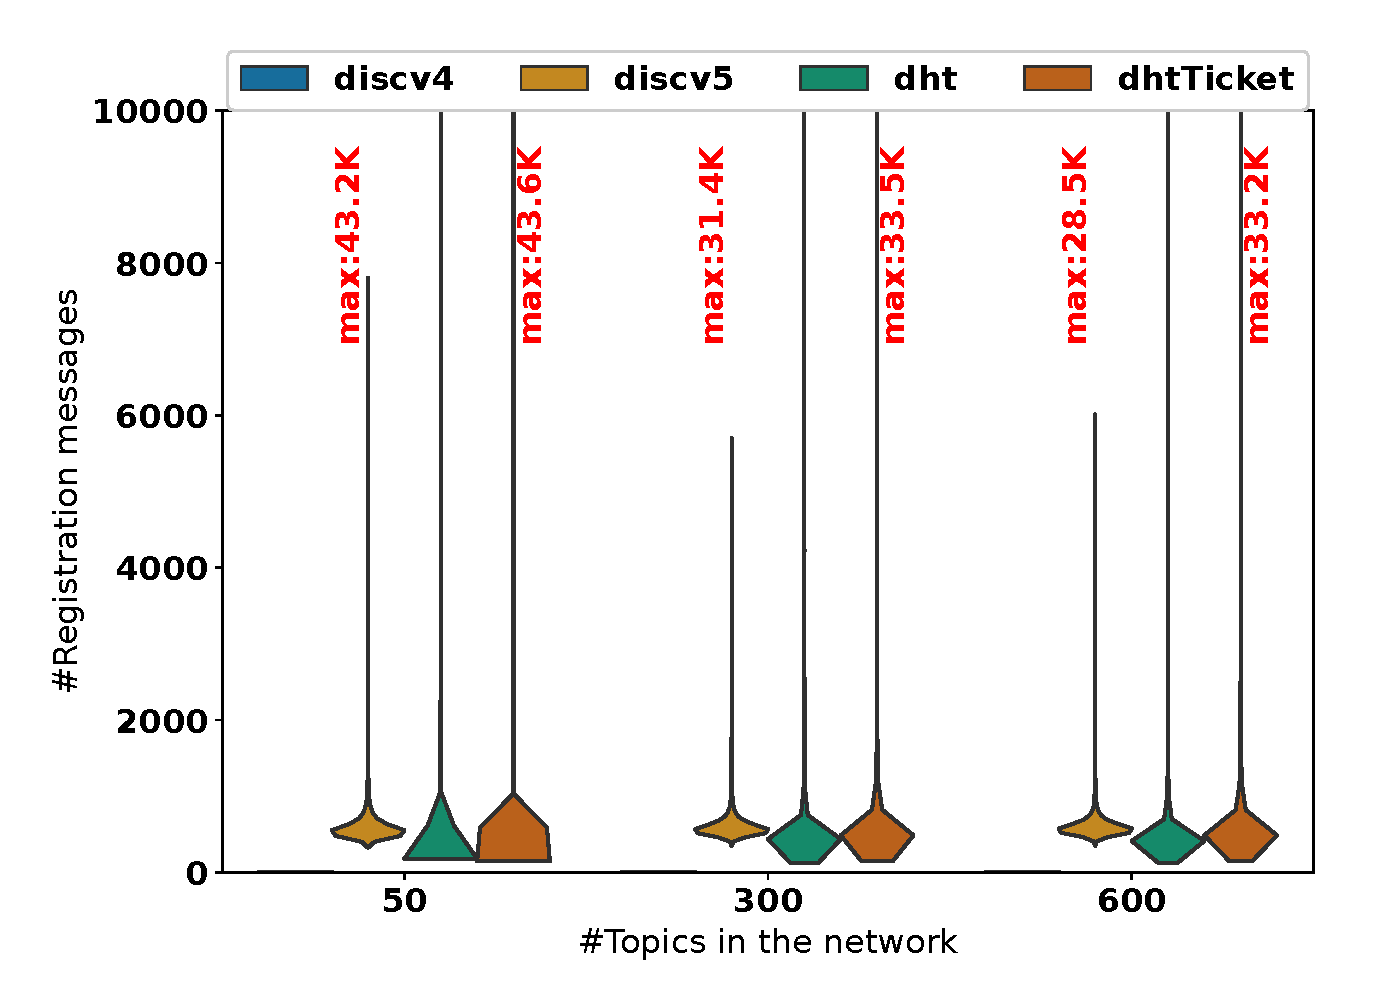
\includegraphics[width=\linewidth]{results/efficiency/violin_topic_registrationMsgs.eps}
%\caption{Y-axis: Distribution of registration related messages received by peers for varying number of topics for the simulation time.}
%\label{fig:regMsgsPerTopic}
%\end{figure}

%In~\Cref{fig:regMsgsPerTopic}~and~\Cref{fig:regMsgsPerSize},  we can observe while most of \sysname nodes receive around 500 registration messages,  with just a few receiving up to 5k messages in the worst case,  \altname solutions are more spread between 0 and 1000 received messages, but with some peaks up to 43k messages,  an order of magnitude higher than \sysname.
%This is caused by the fact that all nodes in \altname solutions try to put registrations starting by the closest nodes to the topic hash,  creating an uneven distribution  towards these nodes. 
%In \sysname, the use of \emph{advertise table} for advertisement placement provides a similar effect. 
%However this effect is diminished by the use of waiting times to regulate advertisement placement.  The increase of waiting time in the more congested nodes, causes that nodes starts more registrations in less congested nodes limiting the number of registrations placed on nodes close to topic hash.
%This effect is not seen when using \altname combined with tickets. 
%This is due to the fact that \altname is not using a \emph{advertise table} to keep track of ongoing registrations.  Because of this,  advertisers start new registrations towards the topic hash every advertisement period, even if they did not succeed in the previous attempts due to high waiting times.
%Therefore using tickets in the \altnameticket, maybe useful to increase the diversity in the \emph{advertise tables} but not for load balancing between nodes.
%
%When increasing the number of topics in the network (\Cref{fig:regMsgsPerTopic}), it is not observed an increase of registration messages for any of the different protocols. 
%However,  when increasing the number of nodes participating in the network (\Cref{fig:regMsgsPerSize}),  also registrations messages received per nodes are increased, as expected.
%But this increase is very different between \sysname and \altname protocols.
%\sr{tbc with specific values}

%\begin{figure}[!h]
%\centering
%\includegraphics[width=\linewidth]{results/split/size_registrationMsgs.eps}
%%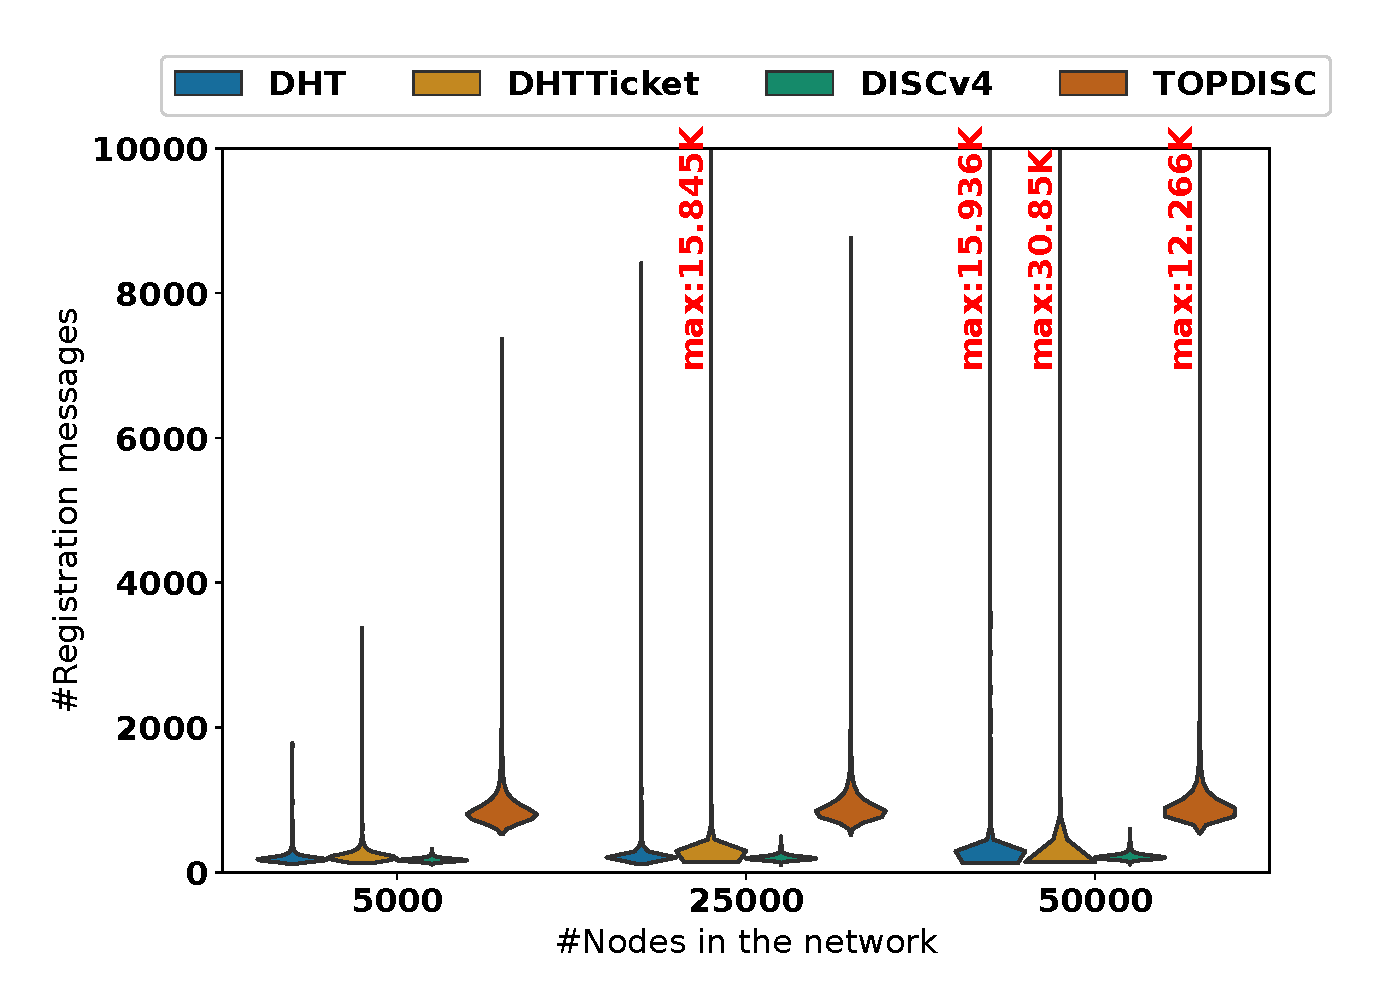
\includegraphics[width=\linewidth]{results/efficiency/violin_size_registrationMsgs.eps}
%\caption{Y-axis: Distribution of registration related messages received by peers for different network size for the simulation time.}
%\label{fig:regMsgsPerSize}
%\end{figure}
%
%\begin{figure}
%\centering
%\includegraphics[width=\linewidth]{results/split/topic_lookupMsgs.eps}
%%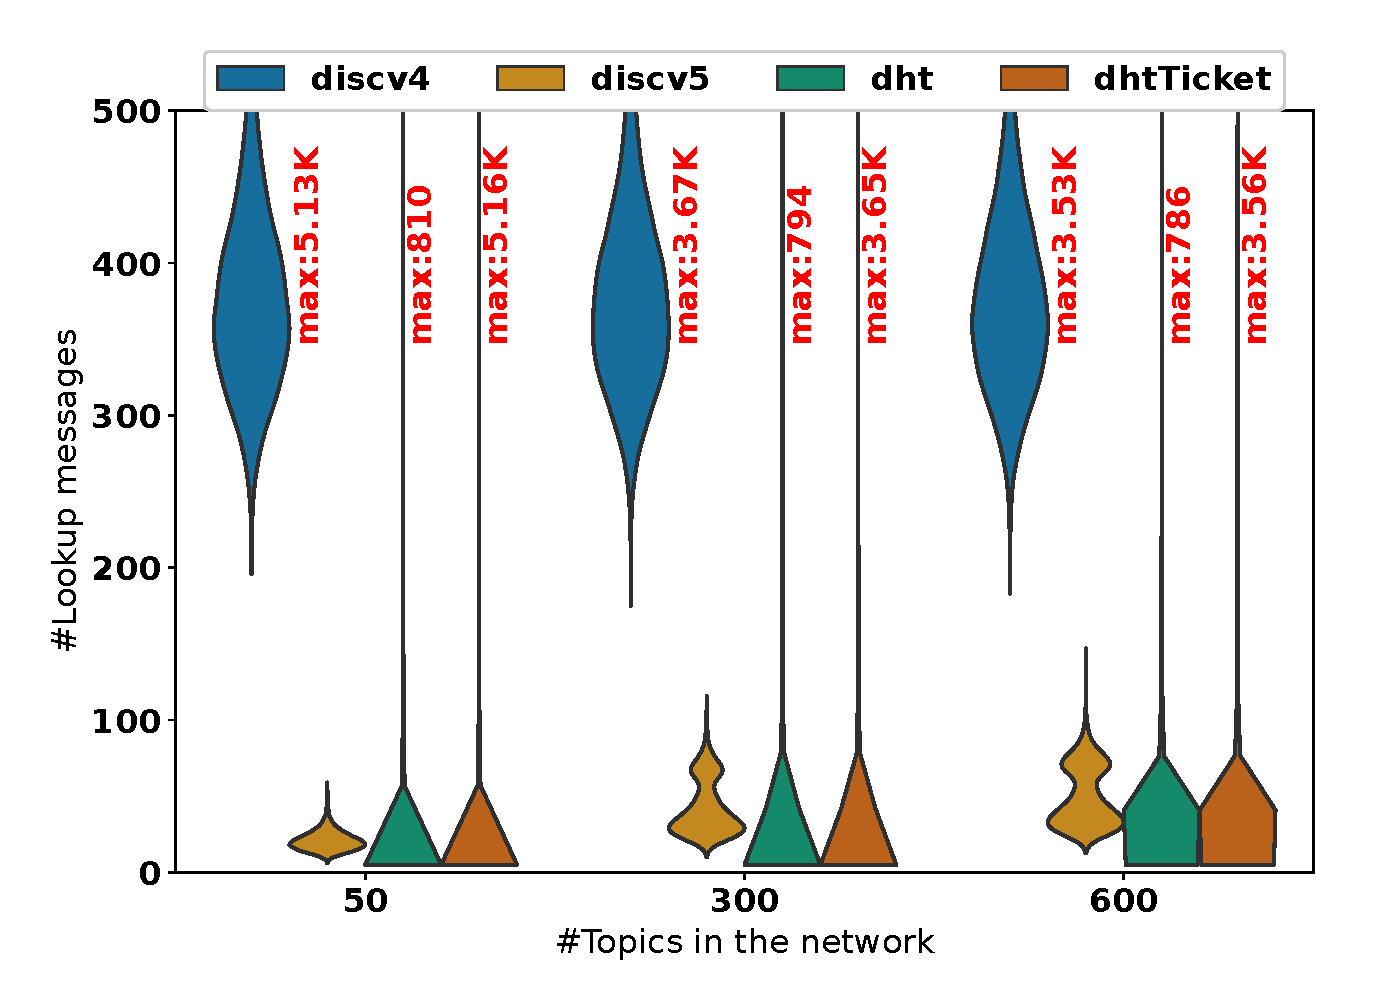
\includegraphics[width=\linewidth]{results/efficiency/violin_topic_lookupMsgs.eps}
%\caption{Y-axis: Distribution of lookup messages received by peers for varying number of topics for the simulation time.}
%\label{fig:lookupMsgPerTopic}
%\end{figure}
%
%\begin{figure}[!h]
%\centering
%\includegraphics[width=\linewidth]{results/split/size_lookupMsgs.eps}
%%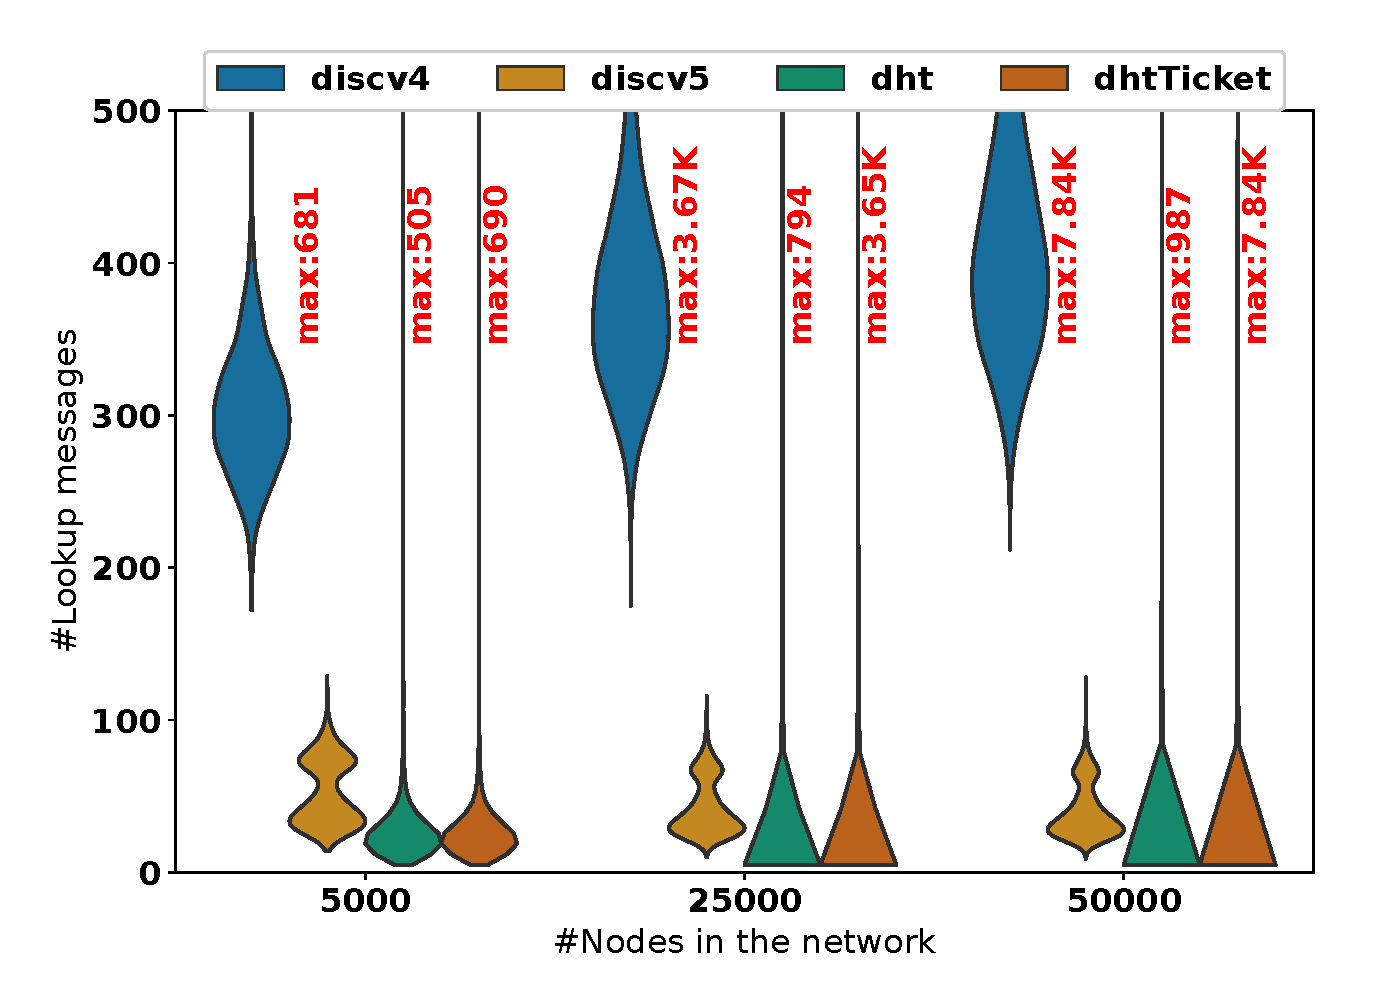
\includegraphics[width=\linewidth]{results/efficiency/violin_size_lookupMsgs.eps}
%\caption{Y-axis: Distribution of lookup messages received by peers for different network size for the simulation time.}
%\label{fig:lookupMsgPerSize}
%\end{figure}

%In~\Cref{fig:lookupMsgPerTopic}~and~\Cref{fig:lookupMsgPerSize}, we observe the number of messages related to the lookup process, \ie topic queries and replies for \sysname, \altname and \altnameticket, and kademlia find/response messages for \discv. We evaluated using  different network sizes and different number of topics in the network. 
%There is a single lookup in the simulation per node, and the $N_\textit{lookup}$ parameter used is equal to 30.  Therefore nodes stop the lookup process when found 30 different nodes in the network for the intended topic.
%In the figures we can observe there is a big different between topic-aware protocols (\sysname, \altname and \altnameticket) and \discv. 
%
%\sr{why there is an increase for \discv with the number of nodes in the simulation and not the number of topics??? shouldn't be the opposite? I guess is because even if there are topics with less nodes there is just a single lookup with the same nodes contacted}
%\sr{why the peak is bigger for DHT for 600 than 300? Is it because of topic hash ids colliding?}

\begin{figure}[!h]
\centering
\includegraphics[width=\linewidth]{results/split/size_totalMsg.eps}
%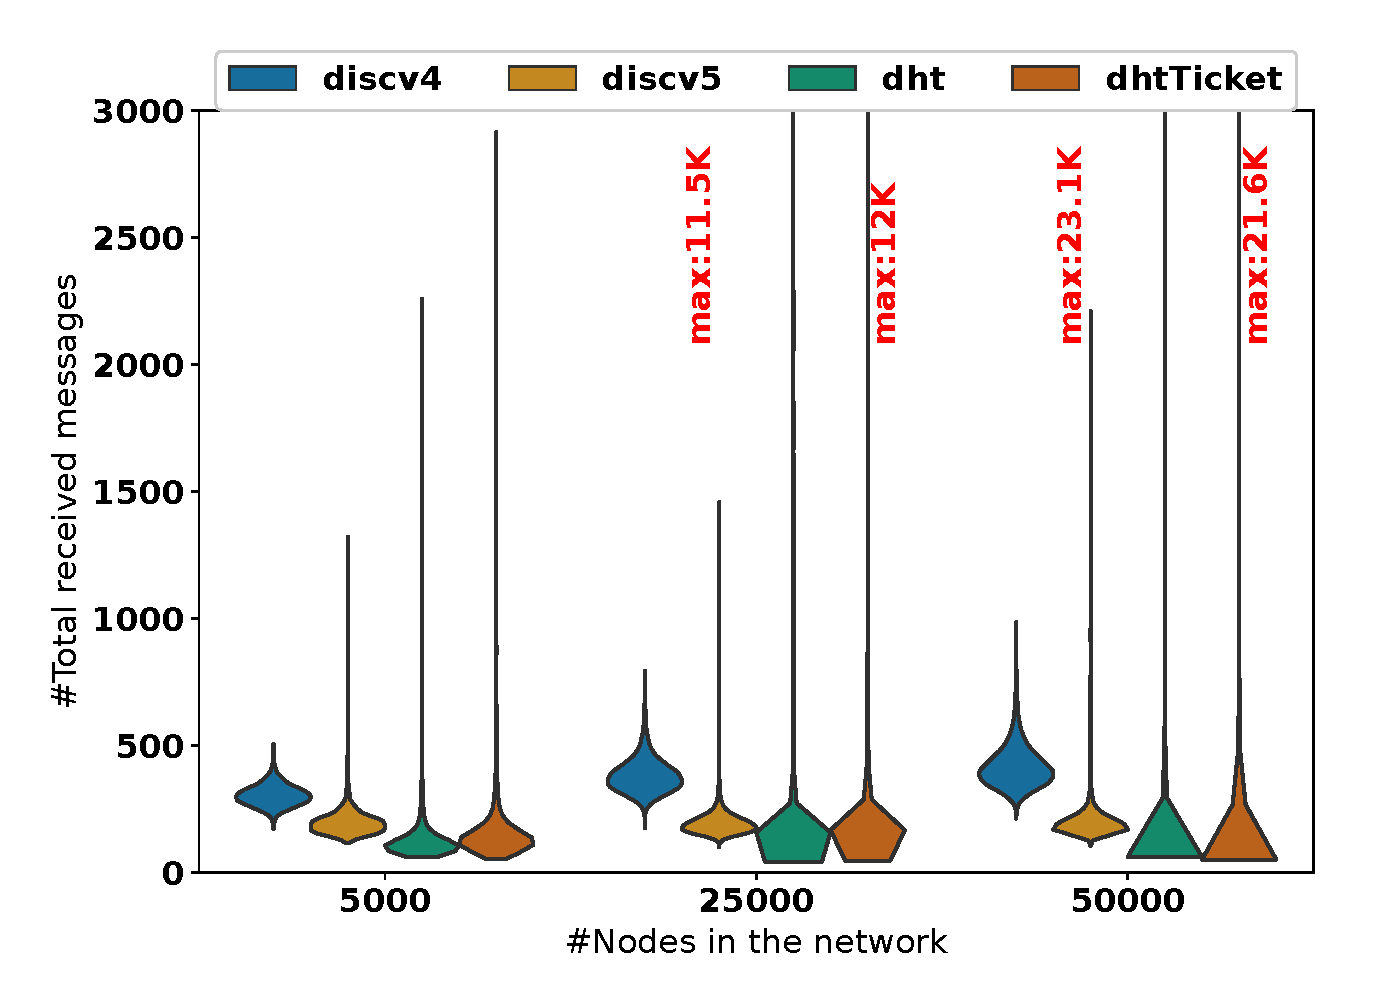
\includegraphics[width=\linewidth]{results/efficiency/violin_size_totalMsg.eps}
\caption{Y-axis: Distribution of discovery related (including registration and lookup) messages received by peers for different network size during a single advertisement period.}
\label{fig:msgsPerSize}
\end{figure}

\begin{figure}
\centering
\includegraphics[width=\linewidth]{results/split/topic_totalMsg.eps}
%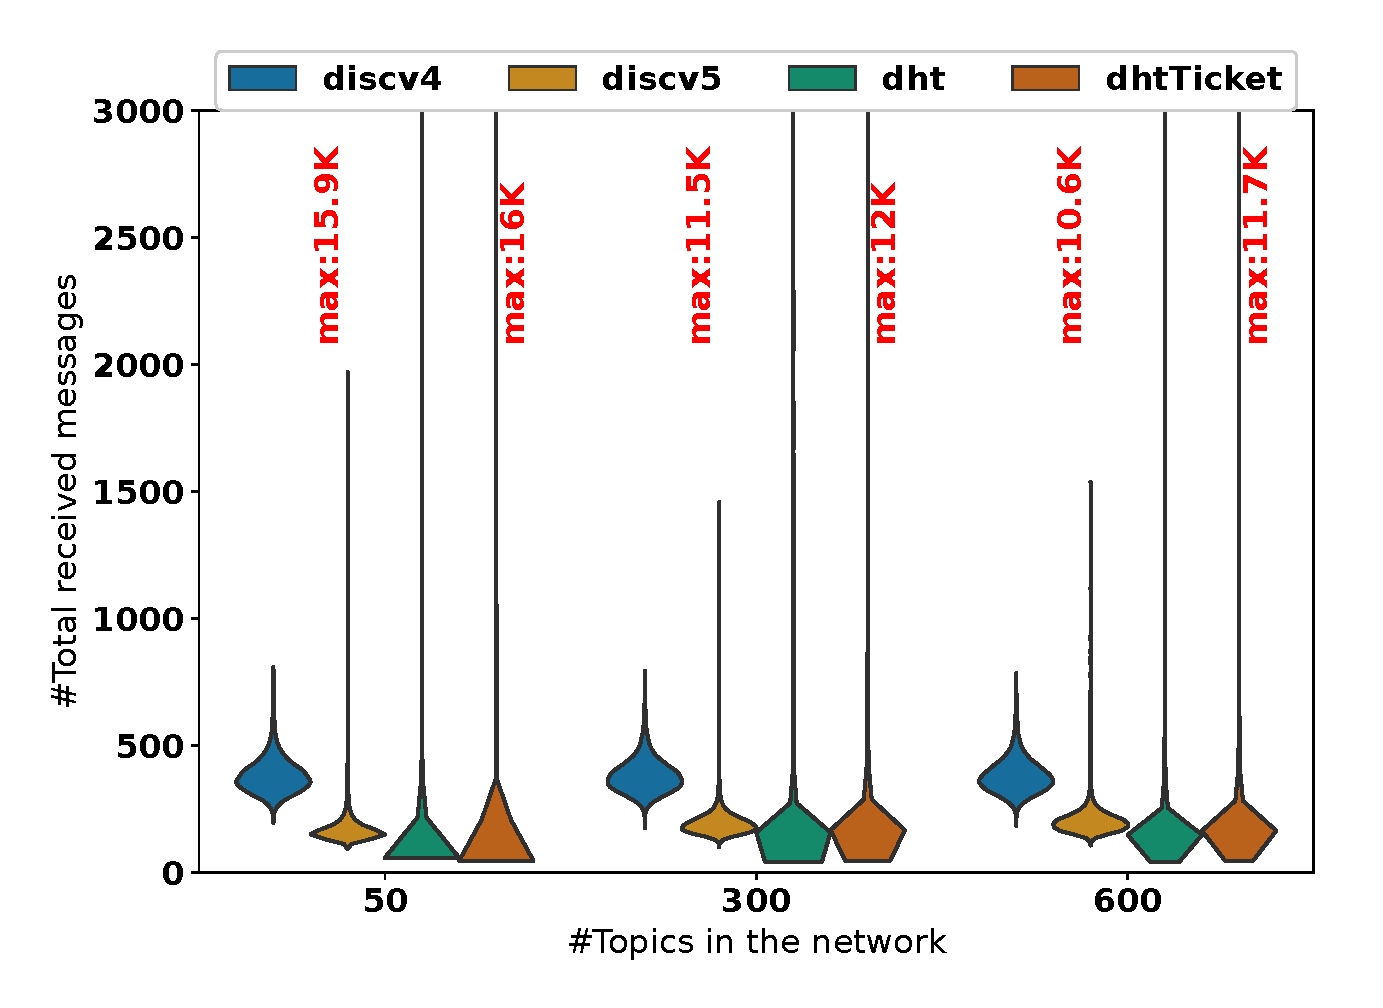
\includegraphics[width=\linewidth]{results/efficiency/violin_topic_totalMsg.eps}
\caption{Y-axis: Distribution of discovery related (including registration and lookup) messages received by peers for different number of topics during a single advertisement period.}
\label{fig:msgsPerTopic}
\end{figure}

In~\Cref{fig:msgsPerSize}~and~\Cref{fig:msgsPerTopic}, we observe the total number of messages during the simulation but normalised per advertisement period. 
Therefore in the figures, it is shown the messages related to a single lookup per node and a single registration process per node before advertisements start to expire and need to be refreshed.
This the overall overhead registered per node in the network.
We can observe that \altname protocols does not scale with the increase of nodes in the network. 
Nodes that are close to a topic hash receive most of the traffic and there is a linear increase with the number of nodes in the network. 
\discv protocol has a better distribution of the load between nodes since its behaviour is completely random. However, the average load in nodes is the highest one because of the overhead caused by not being able to find nodes for specific topics, increasing the overhead during lookup.
\sysname in comparison, provides lower overhead than the other protocols.

%%%%%%%%%%%%%%%%%%%%%%%%%%%%%%%%%%%%%%%%%%%%%%%%%%%%%%%%%%%
\subsection{Lookup performance}

\begin{figure}[!h]
\includegraphics[width=\linewidth]{results/split/topic_discovered.eps}
%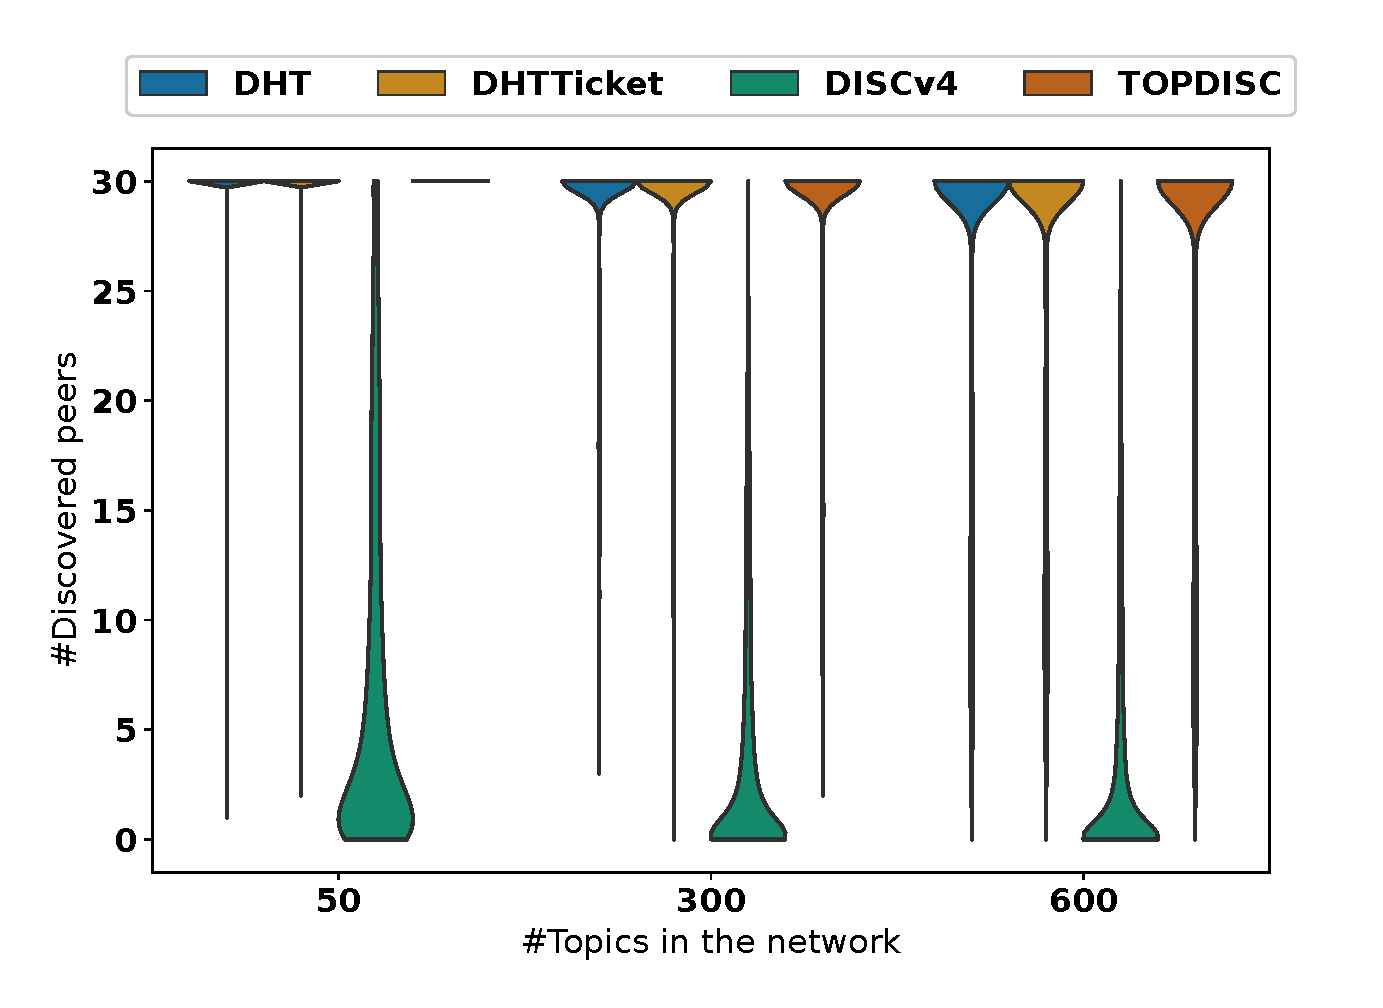
\includegraphics[width=\linewidth]{results/efficiency/violin_topic_discovered.eps}
\caption{Y-axis: Distribution of the number of peers discovered during lookup operation for different number of topics.}
\label{fig:discoveredPerTopic}
\end{figure}

\Cref{fig:discoveredPerTopic} presents the number of peers discovered during a single lookup operation with increasing number of topics in the network. The discovery becomes more difficult, as the number of topics grows.  \discv achieves a much lower number of discovered peers per operation, while \sysname and DHT-based solution efficiently discover the required amount of nodes. The rare cases where \sysname and DHT-based solution do not discover the required amount of peers are caused by small networks that consist of less than 30 nodes. 

\michal{regarding \Cref{fig:discoveredPerTopic}, it seems that for 300 and 600 topics, we discover slightly less peers on average than the DHT solutions. Why is that? Those results should be for the same topic distributions across protocols, right?}
\sergi{I think is normal and is caused by the fact that dht is going straight to nodes with most of the registrations so, specially with topics with very few nodes, they can find nodes faster, but with the tradeoff of being eclipsed very easy.}

\begin{figure}[!h]
\includegraphics[width=\linewidth]{results/split/size_discovered.eps}
%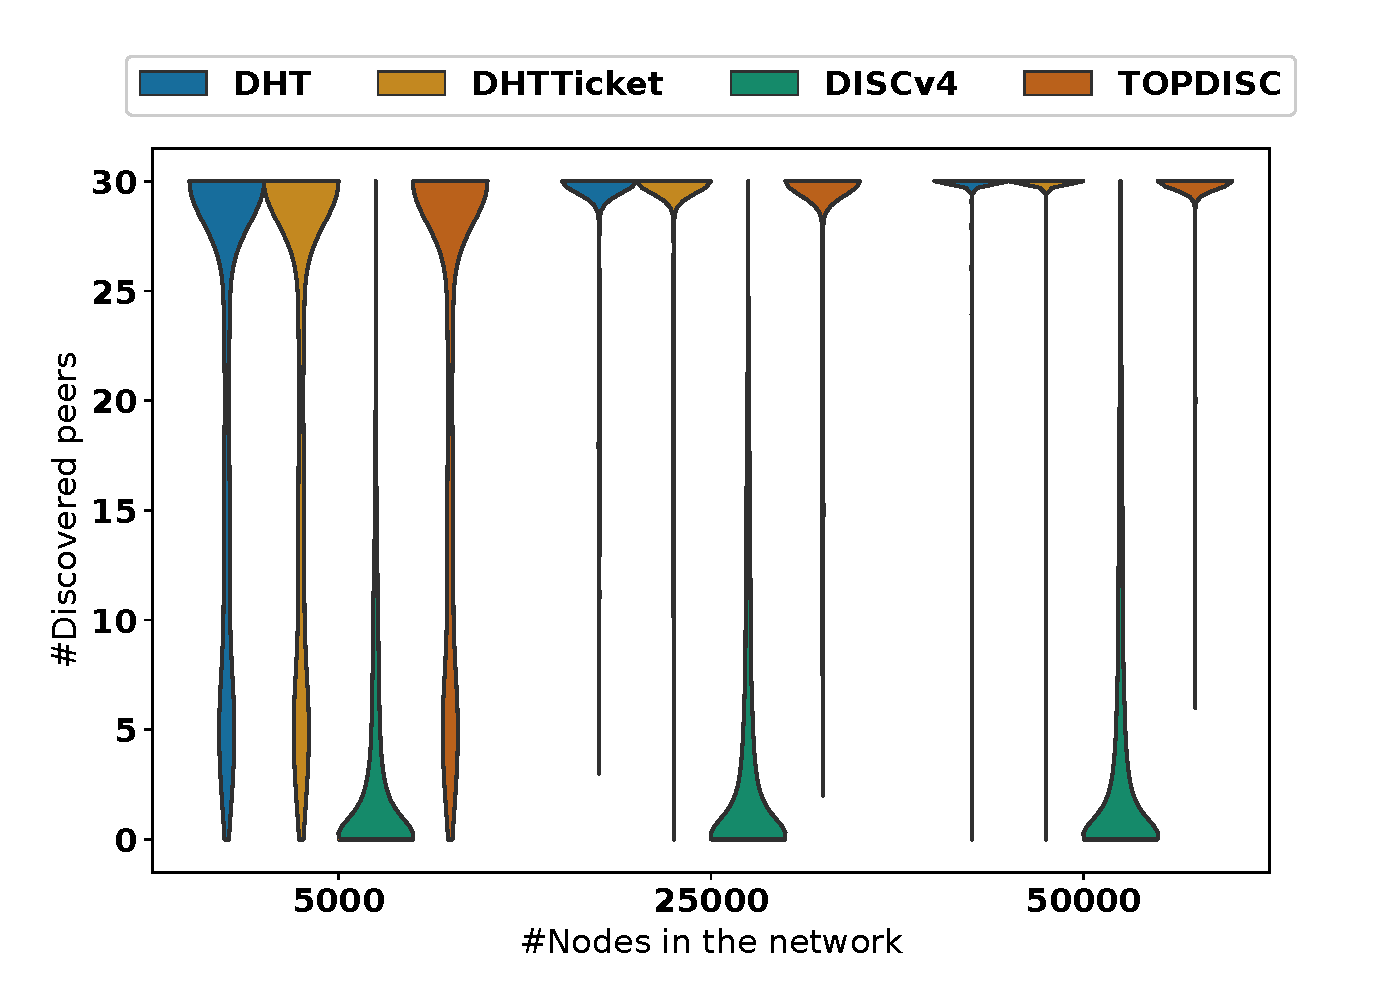
\includegraphics[width=\linewidth]{results/efficiency/violin_size_discovered.eps}
\caption{Y-axis: Distribution of the number of peers discovered during lookup operation for different network size.}
\label{fig:discoveredPerSize}
\end{figure}

\Cref{fig:discoveredPerSize} presents the number of peers discovered during a single lookup operation with increasing size of the network. With a fixed amount of topics, each application-specific network grows and for all the protocols, it is easier to find the required amount of nodes. However, discv4 suffers from poor performance for all the investigated network sizes. 

\begin{figure}
\includegraphics[width=\linewidth]{results/split/topic_wasDiscovered.eps}
%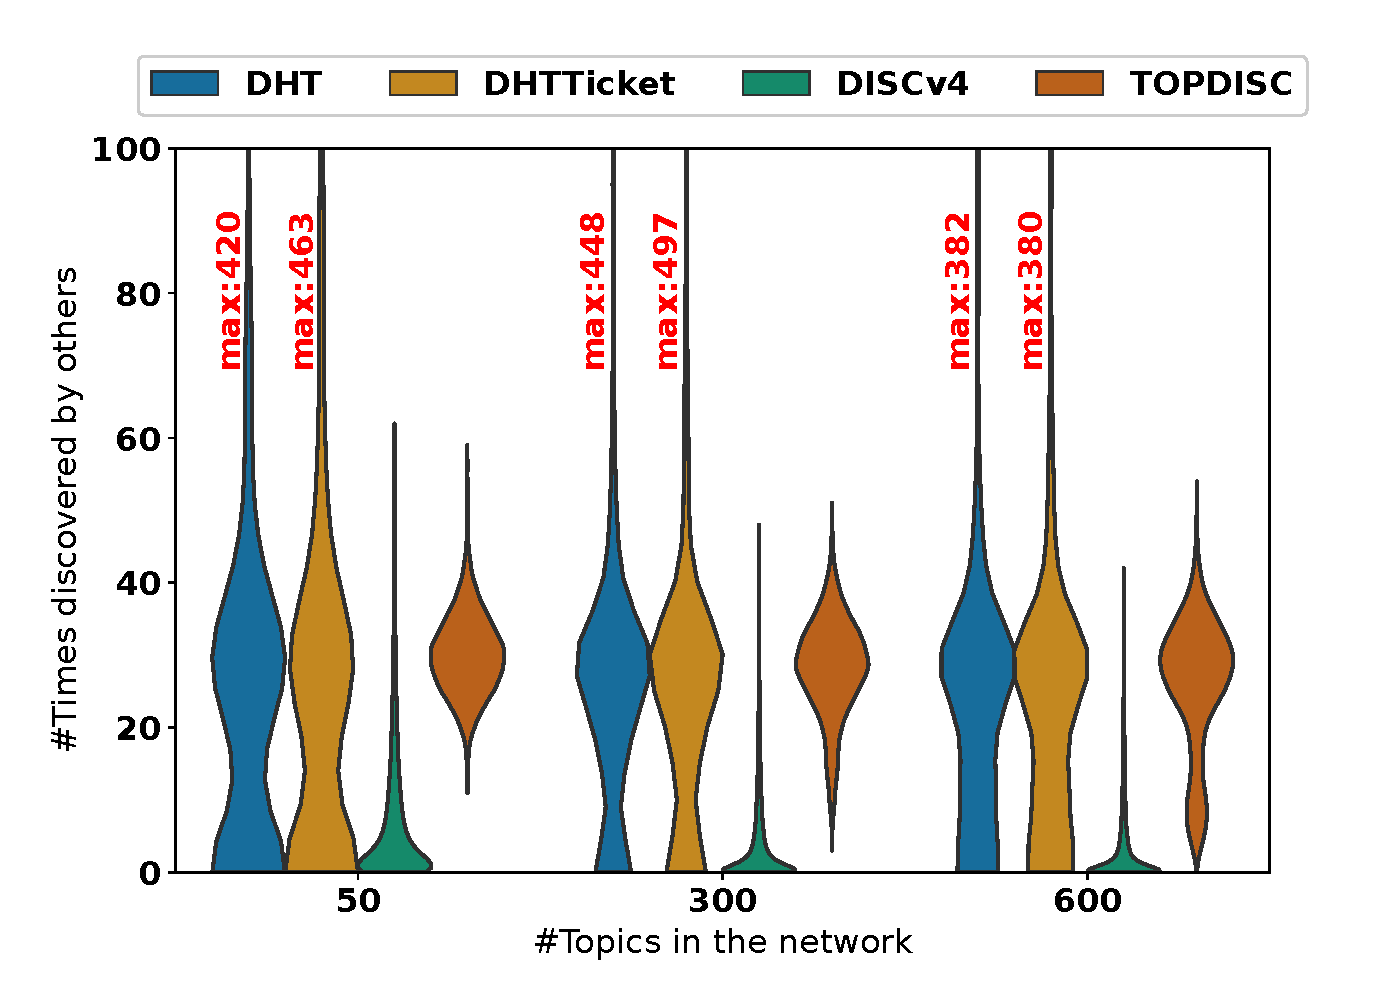
\includegraphics[width=\linewidth]{results/efficiency/violin_topic_wasDiscovered.eps}
\caption{Y-axis: Distribution of the number of times a peer is discovered by others for number of topics in the network for the simulation time.}
\label{fig:discoveredByPerTopic}
\end{figure}

\begin{figure}[!h]
\includegraphics[width=\linewidth]{results/split/size_wasDiscovered.eps}
%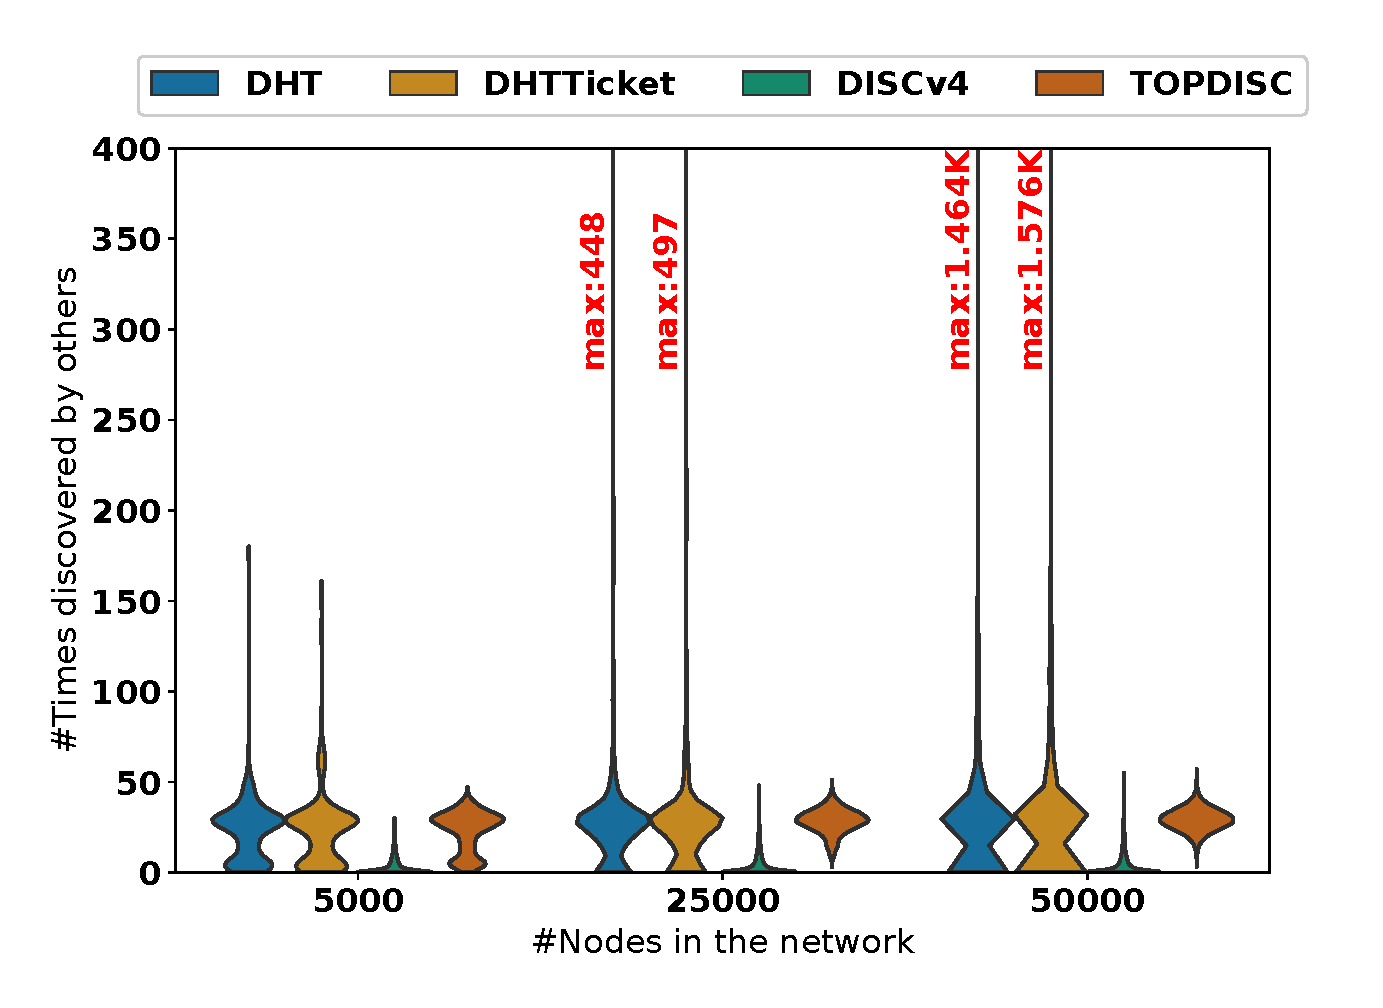
\includegraphics[width=\linewidth]{results/efficiency/violin_size_wasDiscovered.eps}
\caption{Y-axis: Distribution of the number of times a peer is discovered by others for different network size for the simulation time.}
\label{fig:efficiency_size}
\end{figure}

%\subsection{Registrations}
%
%
%\begin{figure}
%\includegraphics[width=\linewidth]{results/split/topic_regsPlaced.eps}
%%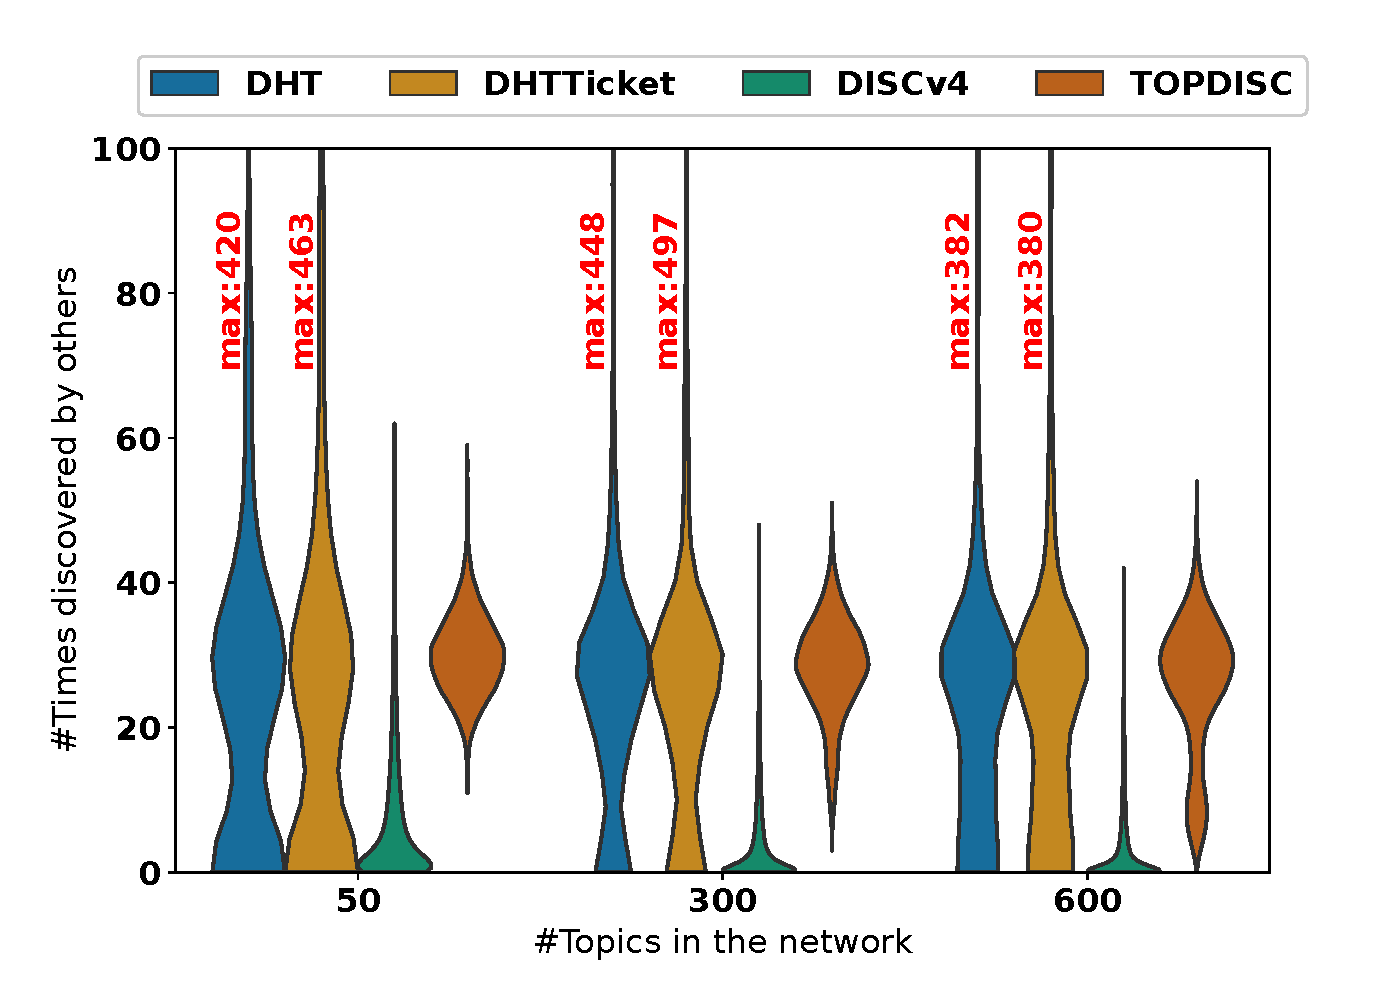
\includegraphics[width=\linewidth]{results/efficiency/violin_topic_wasDiscovered.eps}
%\caption{Y-axis: .}
%\label{fig:regsPlacedPerTopic}
%\end{figure}
%
%\begin{figure}[!h]
%\includegraphics[width=\linewidth]{results/split/size_regsPlaced.eps}
%%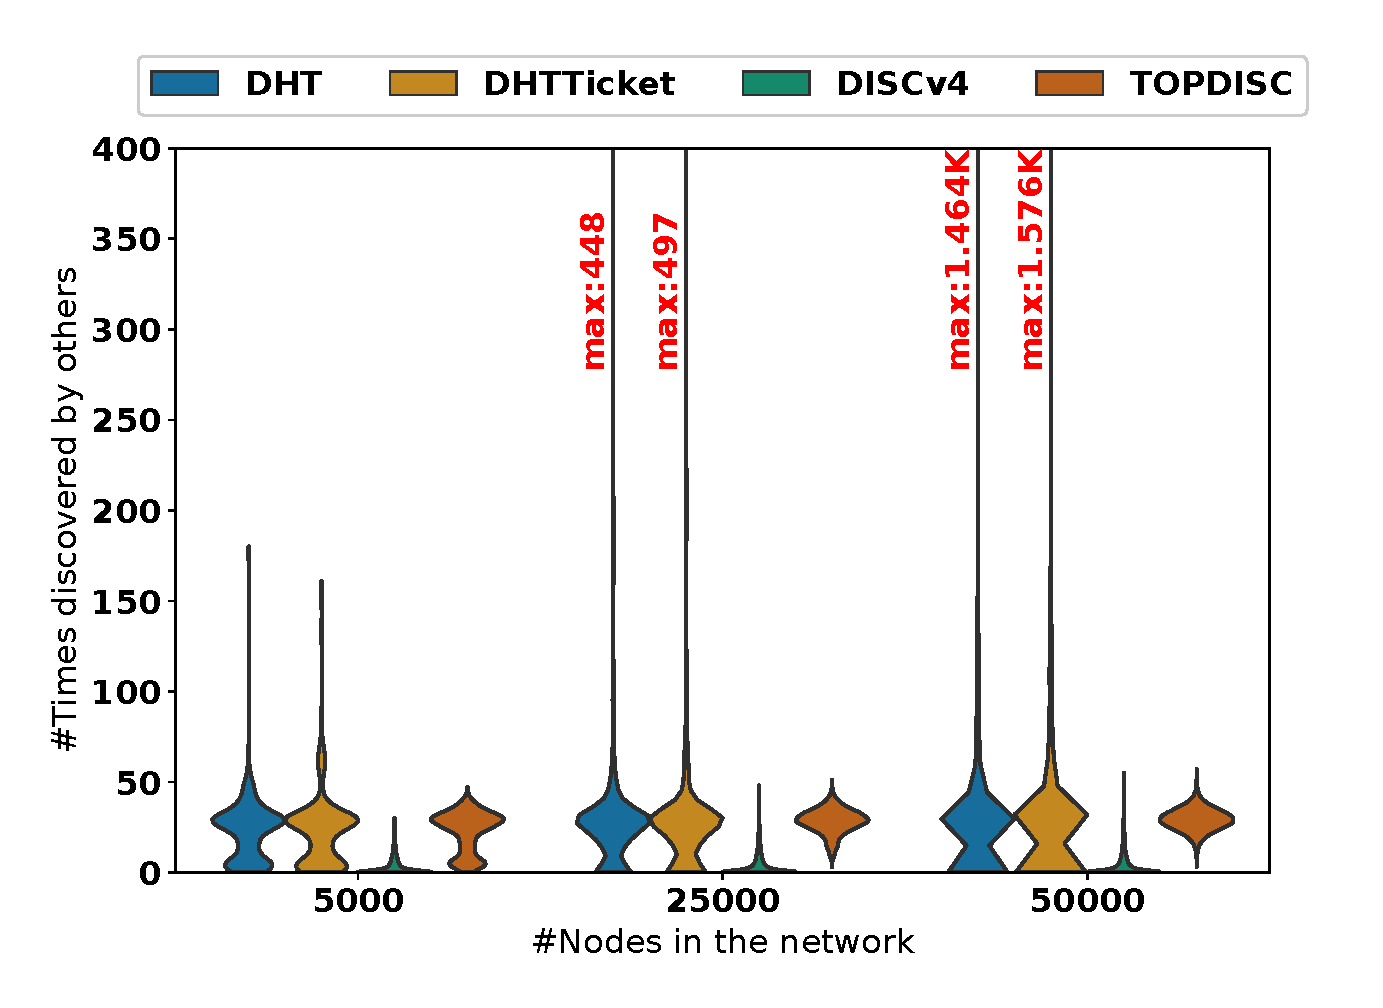
\includegraphics[width=\linewidth]{results/efficiency/violin_size_wasDiscovered.eps}
%\caption{Y-axis: .}
%\label{fig:regsPlacedPerSize}
%\end{figure}
%
%\begin{figure}
%\includegraphics[width=\linewidth]{results/split/topic_regsAccepted.eps}
%%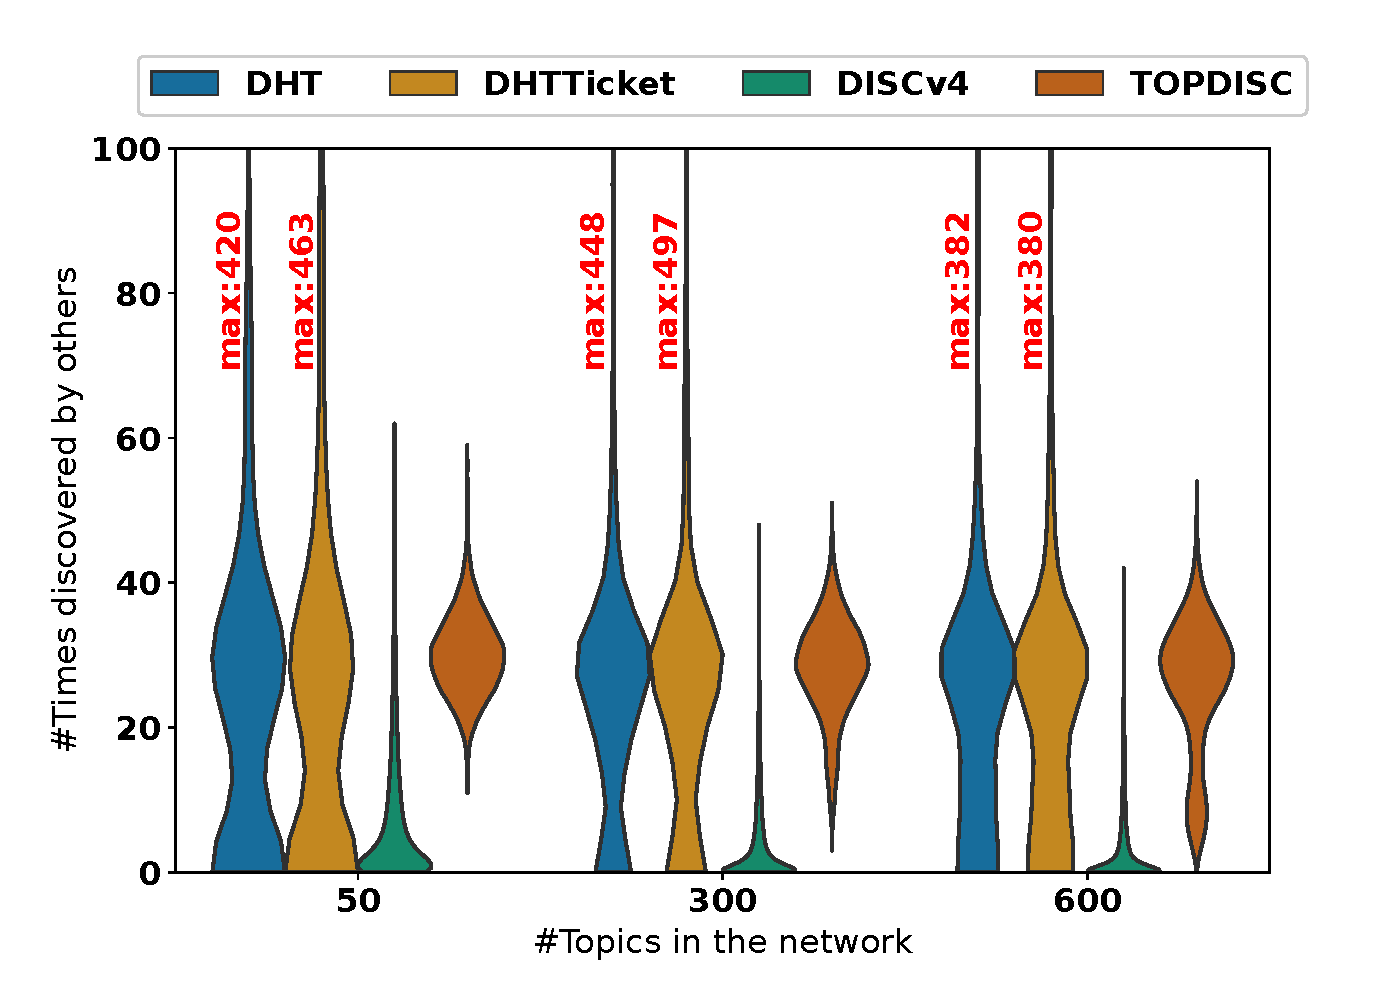
\includegraphics[width=\linewidth]{results/efficiency/violin_topic_wasDiscovered.eps}
%\caption{Y-axis: .}
%\label{fig:regsAcceptedTopic}
%\end{figure}
%
%\begin{figure}[!h]
%\includegraphics[width=\linewidth]{results/split/size_regsAccepted.eps}
%%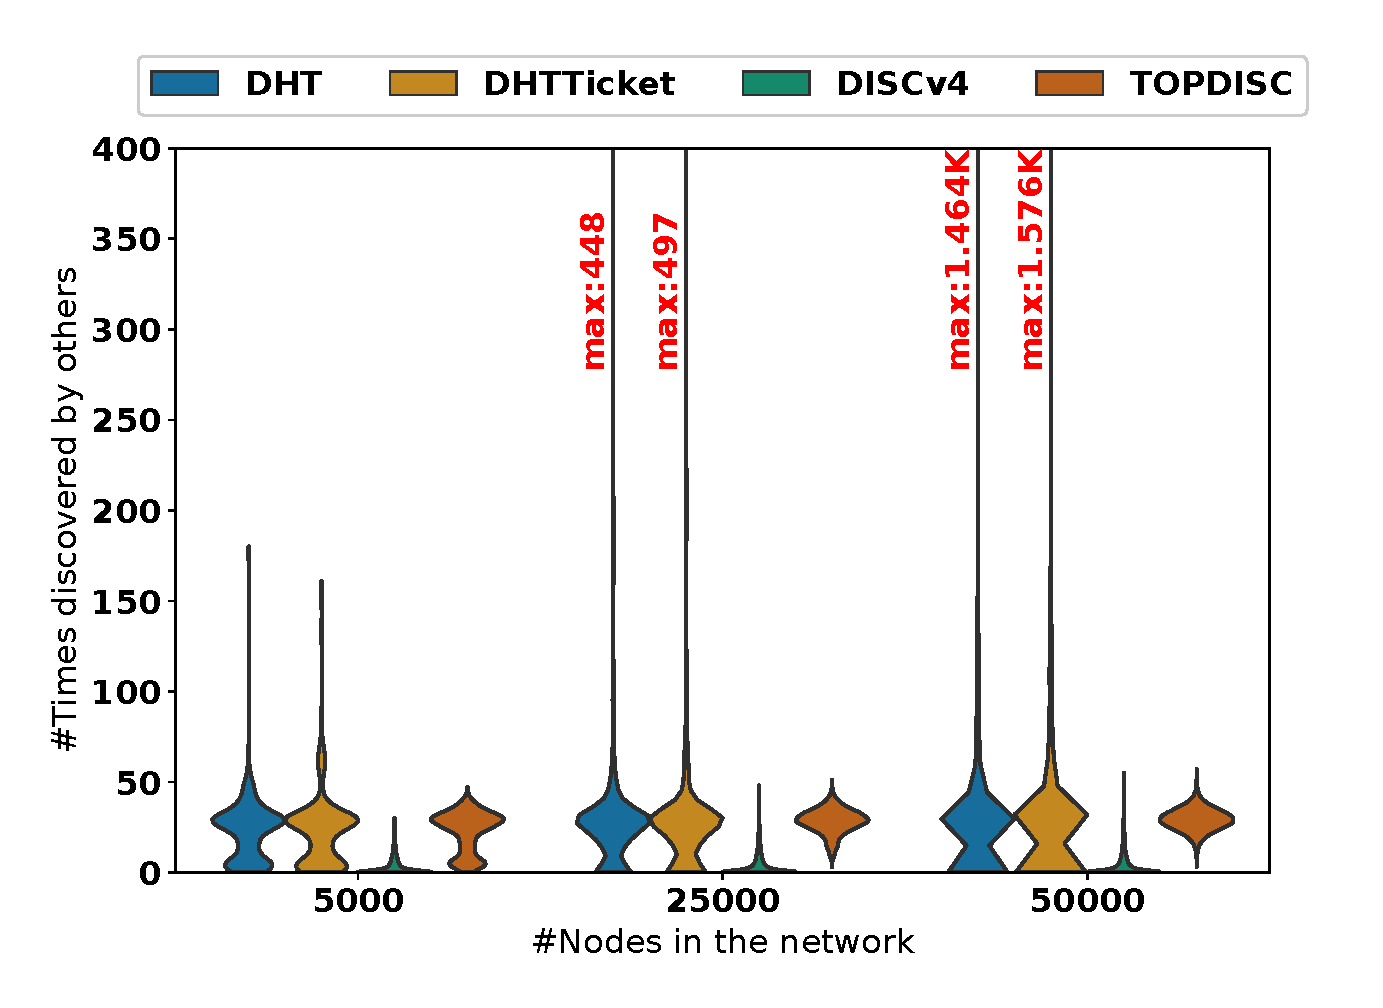
\includegraphics[width=\linewidth]{results/efficiency/violin_size_wasDiscovered.eps}
%\caption{Y-axis: .}
%\label{fig:regsAcceptedSize}
%\end{figure}

\subsection{Security}
%We evaluate \sysname resistance to two groups of malicious attacks:
%\begin{itemize}
%    \item \textbf{Eclipse Attack} - the attacker tries to make a target node discover and connect to peers under the attacker's control. The attack succeeds when all the inbound and outbound connections of the target node are established with malicious peers. 
%    \item \textbf{Denial of Service (DoS)} - the attacker tries to disturb protocol operations. The attack succeeds when service discovery is made impossible or significantly delayed for a group of benign nodes.  
%\end{itemize}
%The attacker may use a large but finite number of malicious nodes. Both attacks may target a single node or a group of nodes (\eg nodes participating in a specific application). 

%\para{Eclipse Attack}

\para{Eclipse Attack}
We implemented and evaluated \sysname resistance against a hybrid eclipse attack targeted to a specific topic,  that  tries to make a searcher node discover and connect to peers under the attacker's control.  
The attacker may be able to generate a large but finite number of Sybil nodes,  with limited network resources (\ie limited IP addresses used by the Sybil nodes pool used in the attack).
The attack succeeds when all the inbound and outbound connections of the target node are established with malicious peers.  The attack consists of the following:
\begin{itemize}
    \item \textbf{Registration spam} - the attacker targets a registrars and sends a large number of registrations requests. If successful, the attacker exhaust registrar's resources and prevent benign nodes from registering. 
%    \item \textbf{Malicious registrar} - the attacker deploys its nodes playing the role of registrars that \textit{(i)} return maximum waiting times when asked for a ticket, \textit{(ii)} return an empty set when asked about a topic. If successful, the attacker prevents benign advertisers from registering \textit{(i)} and prevents benign searchers from discovering their peers \textit{(ii)}. 
	\item \textbf{Malicious registrar} - the attacker deploys its nodes playing the role of registrars that only malicious sybils with the objective of preventing benign searchers from discovering valid peers and eclipsing all its connections.  We consider a coordinated eclipsing attack and any malicious registrar replies with a subset of the identifiers of the Sybil nodes controlled by the attacker.
\end{itemize}

We evaluated the resistance against eclipse attacks using the same default parameters used in the performance evaluation, that is 25000 nodes in the simulation and 300 topics by default, distributed using zipf function of exponent 1.0.  The simulation runs for 1 hour and there is a single lookup per node for the topic it participates.
Nodes get eclipsed when all nodes discovered during a lookup are malicious nodes controlled by the attacker, and therefore they only can connect to the attacker and get the view of the network from the attacker only. 

In the following figures we show violin plots representing the number of malicious nodes returned per lookup using different parameters for the same protocols evaluated in the performance simulations.  On top of each violin plot we specify the percentage of nodes eclipsed after a lookup (\ie percentage of lookups where all nodes returned are malicious nodes).
We evaluated the eclipse attacks targeting two specific topis, the most popular topic and a low popularity topic.
The most popular topic has 3978 nodes registering for this topic and the low popularity has only 33 nodes.
We evaluated the attacks for the most popular and least popular 


\begin{figure}[!h]
\includegraphics[width=\linewidth]{results/security/violin_idDistribution_percentageMaliciousDiscovered_t0.eps}
\caption{Y-axis: Malicious nodes discovered and percentage eclipsed nodes using uniform distributed sybil identities vs generating node ids close to topic id,   when attacking the most popular topic (3978 nodes).}
\label{fig:eclipse_distribution_t0}
\end{figure}

In Figure~\ref{fig:eclipse_distribution_t0} we show the malicious nodes discovered for all lookups for all protocols using different distribution of the identifiers of the malicious nodes,  when attacking the most popular topic (with 3978 nodes).  In the first option, the malicious nodes ids are artificially generated with a small distance to the topic hash id.  In the second option, malicious nodes identifiers are uniformly distributed.  In the figure we can observe that for \altname and \altnameticket the percentage of eclipses are superior to 80\% because most of the nodes close to topics identifiers are nodes controlled by the attacker.  
For \altname and \altnameticket, the lookup process is similar to Kademlia lookup process and,  placing all malicious nodes close the topic hash,  it makes very likely to query only malicious nodes during the process, since it only queries the closest known nodes to the topic identifier.
When attackers are uniformly distributed in the network, eclipses are reduced to close to 32.9\% and 33.7\% respectively.
Even though it is much less likely to hit malicious nodes during the lookup in this case (remember the default number of malicious are 1000 -4\% of the network-),  when hitting a malicious nodes, the nodes returned by them are used to continue the  query and it may happen it continues querying malicious nodes only during the process.
When a low popularity topic is attacked (with only 33 nodes),  as shown in Figure~\ref{fig:eclipse_distribution_t299},  for  \altname and \altnameticket the eclipses are even higher, reaching a 100\% of eclipses when placing malicious nodes close to the topic id, and reaching a 78.8\% and 90.9\% when distributing malicious nodes uniformly.  
Remember the number of attackers is 1000,  against the 33 valid nodes.

For \discv,  the number of eclipses reach is 0\% for the most popular topic when attackers are placed close to the topic hash.  When Sybil nodes are uniformly distributed the number of malicious nodes returned increases,  but to a very low 0.1\%.
This is caused by the fact that \discv does not target lookups to any specific identifier,  but completely random identifiers,  so it is very difficult for the attackers to place Sybil nodes where they will be queried.  Moreover it is difficult by the attackers to send identifiers where the lookup process will be likely to continue to,  because in the FIND node for the Ethereum DHT the lookup identifier is not disclosed,  but only the distance to it.
The number of eclipses reach 12.1.\% for the least popular topic when attackers are placed close to the topic hash.  When Sybil nodes are uniformly distributed the number of malicious nodes returned increases,  however the eclipses  reach a 78.8\%.
The resistance of \discv to Sybil attacks is obtained with the important trade-off of very low efficiency when finding nodes for specific topics, specially for low popular topics.  It is very likely that, when doing lookups using \discv for very low popular topics, no nodes are found or just a few of them.   This means when hitting a malicious node during lookup,  it is likely with a single query to a malicious node, the node querying will be eclipsed.

For \sysname, the number of eclipses are very low for the most popular topic. 
The eclipses are 0\% when Sybil nodes are placed close to topic id and 0.5\% when are uniformly distributed, with similar distribution to the malicious nodes returned compared with \discv.
However when attacking the least popular topic the eclipses increase to 78.8\% for both cases.
This is due to the very low number of valid nodes (33),  that will be more difficult to find than the attackers (1000 nodes, reusing 100 IP addresses).  
But event the high number of attackers in almost half the cases valid nodes are also found along the evil nodes.
Remember that Sybil nodes are completely valid nodes from a network discovery point of view when using different network addresses.

\begin{figure}[!h]
\includegraphics[width=\linewidth]{results/security/violin_idDistribution_percentageMaliciousDiscovered_t299.eps}
\caption{Y-axis: Malicious nodes discovered and percentage eclipsed nodes using uniform distributed sybil identities vs generating node ids close to topic id,   when attacking the low popularity topic (33 nodes).}
\label{fig:eclipse_distribution_t299}
\end{figure}

In Figure~\ref{fig:eclipse_evil_t0} we show the malicious nodes discovered for all lookups for all protocols, using different number of Sybil nodes in the network,  when attacking the most popular topic,  and in Figure~\ref{fig:eclipse_evil_t299} we show the malicious nodes discovered for the least popular topic.  In both figures attackers identifiers are generated uniformly and attackers use a pool of 100 IP addresses. 
In Figure~\ref{fig:eclipse_evil_t0}, we observe \discv is the protocol with the lowest number of eclipses and with the best distribution of malicious nodes returned during lookups.  However \sysname performs very close to \discv, having only 0.2\% of eclipses when there are 1000 attackers in the network.
\altname and \altnameticket has the worst performance,  having 47.7\% and 48.4\% of eclipses when when there are 2500 attackers.
In Figure~\ref{fig:eclipse_evil_t299}, when attacking least popular topic, we observe \sysname is the most resistant to eclipsing.
This is because it is the protocol that is able to discover more nodes with a higher diversity and is the protocol that will find easier the any of the few valid nodes in the network, and therefore it will be not eclipsed.
 
\begin{figure}[!h]
\includegraphics[width=\linewidth]{results/security/violin_percentEvil_percentageMaliciousDiscovered_t0.eps}
\caption{Y-axis: Malicious nodes discovered and percentage eclipsed nodes for different number of sybil nodes used in the attack,  when attacking the most popular topic (3978 nodes).}
\label{fig:eclipse_evil_t0}
\end{figure}

\begin{figure}[!h]
\includegraphics[width=\linewidth]{results/security/violin_percentEvil_percentageMaliciousDiscovered_t299.eps}
\caption{Y-axis: Malicious nodes discovered and percentage eclipsed nodes for different number of sybil nodes used in the attack,  when attacking the low popularity topic (33 nodes).}
\label{fig:eclipse_evil_t299}
\end{figure}


In Figure~\ref{fig:eclipse_sybil_t0} we show the malicious nodes discovered for different number of IP addresses available to the attacker,  when attacking the most popular topic,  and in Figure~\ref{fig:eclipse_sybil_t299} we show the malicious nodes discovered when attacking the least popular topic.
In this case we observe the same results than for the default values. 
\sysname is very close to \discv performance with eclipses closes to 0\% for the most popular topic, and \altname and \altnameticket is close to 33\% eclipses in all cases.
When attacking the low popularity topic,  nodes eclipsed are very similar but having a slight better performance \discv and \sysname.
There is not appreciated in the results any effect of increasing the number of IPs used by the attackers for any of the protocols.
This is caused by the fact that what is more important for the eclipses is whether you hit a malicious node during the lookup process rather than the registrations attackers are able to place in other nodes.

\begin{figure}[!h]
\includegraphics[width=\linewidth]{results/security/violin_sybilSize_percentageMaliciousDiscovered_t0.eps}
\caption{Y-axis: Malicious nodes discovered and percentage eclipsed nodes for different number IP addresses used in the attack,  when attacking the most popular topic (3978 nodes).}
\label{fig:eclipse_sybil_t0}
\end{figure}



\begin{figure}[!h]
\includegraphics[width=\linewidth]{results/security/violin_sybilSize_percentageMaliciousDiscovered_t299.eps}
\caption{Y-axis: Malicious nodes discovered and percentage eclipsed nodes for different number IP addresses used in the attack,  when attacking the least popular topic (33 nodes).}
\label{fig:eclipse_sybil_t299}
\end{figure}



%\begin{figure*}[!h]
%\centering
%\subfigure[{Y-axis: Percentage eclipsed nodes using uniform distributed sybil identities vs generating node ids close to topic id}]{
%\includegraphics[width=0.31\textwidth]{results/security/%bar_idDistribution_percentageEclipsedLookups_t0.eps}
%violin_idDistribution_percentageMaliciousDiscovered_t0.eps}
%\label{fig:distribution}
%}
%\subfigure[{Y-axis: Percentage eclipsed nodes for different number of sybil nodes in the attack.}]{
%\includegraphics[width=0.31\linewidth]{results/security/%bar_percentEvil_percentageEclipsedLookups_t0.eps}
%violin_percentEvil_percentageMaliciousDiscovered_t0.eps}
%\label{fig:percentEvil}
%}
%\subfigure[{Y-axis: Percentage eclipsed nodes for different number IP addresses used in the attack.}]{
%\includegraphics[width=0.31\linewidth]{results/security/%bar_sybilSize_percentageEclipsedLookups_t0.eps}
%violin_sybilSize_percentageMaliciousDiscovered_t0.eps}
%\label{fig:sybilsize}
%}
%\caption{Resistance against eclipse attacks when attacking most popular topic (t0)} 
%\label{fig:eclipse_attack}
%\vspace{-0.05in}
%\end{figure*}
%
%\begin{figure*}[!h]
%\centering
%\subfigure[{Y-axis: Percentage eclipsed nodes using uniform distributed sybil identities vs generating node ids close to topic id}]{
%\includegraphics[width=0.31\textwidth]{results/security/%bar_idDistribution_percentageEclipsedLookups_t299.eps}
%violin_idDistribution_percentageMaliciousDiscovered_t299.eps}
%\label{fig:distribution}
%}
%\subfigure[{Y-axis: Percentage eclipsed nodes for different number of sybil nodes in the attack.}]{
%\includegraphics[width=0.31\linewidth]{results/security/%bar_percentEvil_percentageEclipsedLookups_t299.eps}
%violin_percentEvil_percentageMaliciousDiscovered_t299.eps}
%\label{fig:percentEvil}
%}
%\subfigure[{Y-axis: Percentage eclipsed nodes for different number IP addresses used in the attack.}]{
%\includegraphics[width=0.31\linewidth]{results/security/%bar_sybilSize_percentageEclipsedLookups_t299.eps}
%violin_sybilSize_percentageMaliciousDiscovered_t299.eps}
%\label{fig:sybilsize}
%}
%\caption{Resistance against eclipse attacks when attacking least popular topic (t299)} 
%\label{fig:eclipse_attack}
%\vspace{-0.05in}
%\end{figure*}
%\begin{figure}[!h]
%\includegraphics[width=\linewidth]{img/placeholder}
%\caption{Compare only against DHT here I guess? Y-axis a ratio of popular malicious and benign ads in the table for spam attack and topic-targeted attack within a single registrar. X-axis: to avoid showing different graphs for multiple malicious IPs/IDs/nodes we can have a fix ratio between them i.e., each 5 Sybils (or requests/s) have 1 IP and 2 ID, and increase this "attacker strength".} 
%\label{fig:security_spam}
%\end{figure}
%
%\begin{figure}[!h]
%\includegraphics[width=\linewidth]{img/placeholder}
%\caption{Compare only against DHT here I guess? Y-axis a  time to discovery/registration (do we care about registration if lookup works?) slowdown compared to a non-attack scenario?Do we consider different placements of Sybils here (i.e., only bucket 1? Or spread evenly across all the buckets?). X-axis: to avoid showing different graphs for multiple malicious IPs/IDs/nodes we can have a fix ratio between them i.e., each 5 Sybils have 1 IP and 2 ID, and increase this "attacker strength".} 
%\label{fig:security_spam}
%\end{figure}



\iffalse
\subsection{Performance Results}
\michal{We should group the result so that they show achievement of specific goals that we described before}

%\paragraph{Ticket registrations:
In the following we detail the performance evaluation in four different subsections.  In the first we show the registration performance.  Secondly we show the traffic load and overhead of the designed mechanism.  Then we continue with the lookup and discovery performance and we finish with the security analysis.

\subsubsection{Registration  performance}

In Figure~\ref{fig:regs} we observe the average active registrations in the system per topic with different number of nodes in the simulation,  from 500 to 10000 nodes. 
We can observe nodes for all topics are able to place a substantial amount of registrations, even the less popular topics. 
As number of nodes increase in the network, we can observe the differences between registrations per topic are reduced. 
Actually, it can be observed the most popular topic (t1) is able to place less registrations than t2. 
This is caused by the fact that with more nodes trying to register for the same topic,  waiting times increase.
If the waiting time increases over the waiting time limit (in the simulations is set to 15 min),  the node cancels the registration and tries with a different nodes.
When cancellations happen it may lead to less active registrations, because it may end up with longer registration processes.
In our simulation we observe less registrations for t1 than t2  because t1 registrations waiting time go over the waiting time limit more often.

In Figure~\ref{fig:time_reg} we observe the average time necessary for a node to place a registration,  from 500 to 10000 nodes in the simulation.
We can observe that average registration time is always below 500 seconds and this is reduced for less popular topics and smaller networks. 
This figure does not include registration times for cancelled registrations.
\sergi{I think we should include failed/uncomplete registrations in the plot}

\begin{figure}[!h]
\centering
\subfigure[{Active registrations}]{
\includegraphics[width=0.225\textwidth]{img/eval/registration_origin.eps}
\label{fig:regs}
} 
\hspace{-0.25cm}
\subfigure[{Time to register}]{
\includegraphics[width=0.225\textwidth]{img/eval/avg_time_register.eps}
\label{fig:time_reg}
}
 \caption{Ticket registrations} 
\label{fig:registrations}
\vspace{-0.15in}
\end{figure}   

%\begin{figure}[h!]
%\centering
%%\epsfig{file=imgs/eval/scen5.pdf, width=0.45\textwidth}
%\includegraphics[width=0.225\textwidth]{img/eval/registration_origin.png}
%\caption{Registrations}
%\label{fig:regs}
%\vspace{-0.15in}
%\end{figure}

%\paragraph{\bf{Network load}:}
\subsubsection{Network load}

In Figure~\ref{fig:messages}~and~\ref{fig:msg_distr} we can observe the traffic load generated in the network.
In Figure~\ref{fig:messages} we observe most of the messages are ticket requests/replies, and the subsequent registration request/replies
after receiving a ticket from a node. 
This is caused by the fact that nodes are constantly registering dynamically. 
In Figure~\ref{fig:msg_distr} the messages received distribution. 
We can observe some nodes receive much more messages.
This is caused by the bucket node distribution, where nodes with identifiers close to topic hash ids receive more initial tickets requests because there are less.
However, we observe while the number of nodes in the network is increased 20 times,  the  maximum number of messages received by some nodes does not increase in the same way,  only being twice the amount when comparing 500 with 10000 nodes,  ans with increases lower than 30\% when number of nodes are doubled.
Moreover,  we can also see the number of messages received does not exceed 10 times the average value of the messages received. 

Therefore, the system is able to scale without danger of overloading some of the nodes of the network.

\begin{figure}[!h]
\centering
\subfigure[{Number of messages}]{
\includegraphics[width=0.225\textwidth]{img/eval/message_quantity.eps} 
\label{fig:messages}
} 
\hspace{-0.25cm}
\subfigure[{Message distribution}]{
\includegraphics[width=0.225\textwidth]{img/eval/messages_received.eps} %\hspace{-1.5em}%
\label{fig:msg_distr}
}
 \caption{Traffic load} 
\label{fig:traffic}
\vspace{-0.15in}
\end{figure}   

\subsubsection{Discovery and lookup performance}

%\paragraph{\bf{Discovery performance}:}

In Figure~\ref{fig:reg_disc} and \ref{fig:timedisc} we can observe how nodes are discovered within the network.
In Figure~\ref{fig:reg_disc} we observe the percentage of the nodes in the network that are discovered and how often are discovered.
Each node in the network is represented by a circle, and the size of the circle represents the relative frequency of discoveries compared with other nodes in the network.
We can observe that for all topics the percentage of nodes discovered in the network is very close to 100\%. This means almost all nodes in the network are able to be discovered by other nodes. The number of discovered nodes is not 100\% because of the existence of turbulence (there are some nodes just joined the network and there has not been enough time yet to be discovered). In case there are a low number of nodes for a specific topic (e.g. t5 with 500 nodes network) the 100\% is reached.
We can also observe Figure~\ref{fig:reg_disc} that the discovery distribution is bounded to \hl{X} times between the most discovered and the least discovered.
We observe the dots size are very regular and despite being not completely equal the differences are not substantial. 
In Figure~\ref{fig:timedisc} we observe the time between a registration is completed and the first time the registration
is returned in a lookup.
By observing this we can see how difficult is for a node to be discovered once is able to place a registration. 
We see the average time is between 20 and 10 seconds in most of the cases, except for the least popular topic t5 which is around 50\% higher. 
We also observe the deviation is bounded at around 60 seconds, with equivalent different for t5.


\begin{figure}[!h]
\centering
\subfigure[{Advertiser discovery distribution}]{
\includegraphics[width=0.225\textwidth]{img/eval/registrant_distribution.eps} 
\label{fig:reg_disc}
} 
\hspace{-0.25cm}
\subfigure[{Time between registration and first discovery}]{
\includegraphics[width=0.225\textwidth]{img/eval/min_time_discovery.eps} %\hspace{-1.5em}%
\label{fig:timedisc}
}
 \caption{Discovery performance} 
\label{fig:discovery}
\vspace{-0.15in}
\end{figure}   


In Figure~\ref{fig:hopcount} we can observe the lookup performance of \sysname compared with Discv4 for a 5000 nodes simulation.
In the plot we show the average number of nodes discovered for each hop during a lookup per topic, taking into account that Discv4 cannot do per topic lookups,  so we discard received nodes that do not support the specific service.
In the figure we observe that for t1 the discovered nodes are higher when using Discv4, since all topics support t1 and any node discovered will be a valid node. 
However, as the popularity of the topic decreases it also does the lookup performance of Discv4,  since it is very difficult to find nodes for non-popular topics without supporting per topic lookups.
In this sense,  Discv5 lookup performance also decreases the performance with non-popular topics (simply because there are less nodes in the network) however this decrease is diminished.  Between t1 and t5 the lookup performance is decrease approximately to a 1/2th for Discv5, while when using Discv4 the lookup performance decreased to a less than a 1/10th.

%TODO add lookup description including mechanisms to avoid sybils.

\begin{figure}[h!]
\centering
%\epsfig{file=imgs/eval/scen5.pdf, width=0.45\textwidth}
\includegraphics[width=0.35\textwidth]{img/eval/lookup_hopcount_discv4.png}
\caption{Lookup performance}
\label{fig:hopcount}
\vspace{-0.15in}
\end{figure}

\subsubsection{Sybil Attacks}

In the following we show the results of the performance evaluation of the discovery service under different sybil attacks.  The attacks that we evaluated in this section are of two types and are previously described in Section~\ref{sec:overview}. 
These attacks are eclipsing  and Denial-of-service (DoS) attacks.
Eclipsing attacks goal is to generate multiple fake identities within a topic to be able to eclipse existing nodes in the network.
Eclipsing a node imply all outbound and inbound connections are established to only sybil/fake nodes controlled by an attacker.
This allows the attacker to control the view of the network of the eclipsed node and can be used to co-opt a victim's mining power and use it to attack the blockchain's consensus algorithm.
DoS attacks instead is an attack meant to hamper the good performance or even to shut down the network, making it inaccessible to its intended users.  
In our case,  the goal of DoS attacks is to difficult or to block the discovery of nodes in the network and is specially important for topic with low popularity where finding all node in the network is very important.

In the implemented topic eclipsing attack,  malicious nodes are sybil nodes that cooperate in order to eclipse other valid nodes.
Malicious and valid nodes have the same amount of bandwidth resources and malicious nodes respond to topic lookup requests and find messages with only other malicious nodes.
Malicious nodes also act as evil 'advertisers' trying to place as many registrations as possible by using bigger ticket size,  with malicious registrars attack,  where evil registrars replies with only malicious nodes when receiving a topic query.

We implemented and evaluated two kind of DoS attacks.  
The first attack consists in a topic spam attack where a big number of sybil identities generated try to register for non-existing random topics.
By registering for non-existing topics,  evil nodes try to harm valid topics registrations, overflowing ad caches.
The second DoS attack consists on generating sybil identities that keep without replying when receiving valid nodes ticket requests or return very long waiting times. 
This way an attacker can try to backlog valid nodes ticket registrations.

In Figures~\ref{fig:reg_eclipse},~\ref{fig:discoverytime_eclipse}~and~\ref{fig:lookup_eclipse} we show performance results under a
topic eclipsing attack.
We compare results for topic eclipsing attacks targeted to the most popular topic (t1) and attacks targeted to the least popular topic (t5). 
In the simulation there are 2000 nodes, all of them participating in t1 and only 218 participating in t5. 
In the simulations there are an additional 20\% (400 in total) malicious nodes that target the specific topic and the number of resources used in the attack (IP addresses) vary from 1 address to 50.

\begin{figure}[!h]
\centering
\subfigure[{Active registrations eclipse attack t1 attack}]{
\includegraphics[width=0.22\textwidth]{img/eval/attack/registration_origin_t1.eps} 
\label{fig:reg_eclipse_t1}
} 
\hspace{-0.15cm}
\subfigure[{Active registrations eclipse attack t5 attack}]{
\includegraphics[width=0.22\textwidth]{img/eval/attack/registration_origin_t5.eps} %\hspace{-1.5em}%
\label{fig:reg_eclipse_t5}
}
 \caption{Active registrations under topic eclipsing attack} 
\label{fig:reg_eclipse}
\vspace{-0.15in}
\end{figure}   

In Figure~\ref{fig:reg_eclipse_t1} we observe the active registrations in the simulation per topic, for an eclipsing attack targeted to the most popular topic (t1), including active registrations of malicious nodes.
We can observe than even though the number of malicious nodes is equivalent to 20\%, the number of active registrations is lower than that. 
As expected, as the number of IP addresses used in the attack increaseas, the number of active registrations of malicious nodes also increase, since different malicious nodes with complete different IPs can not be diffierentiated from valid nodes.
For topic 5, the most vulnerable topic for being the least popular, we can observe a similar pattern of active registrations. 
However, we observe that despite malicious nodes being more (400 nodes) than valid nodes (218 nodes), active registrations of malicious nodes is kept lower than 30\% in all cases. Similarly to t1, the active registrations increase with the higher number of IPs used in the attack, since there is no way to a totally distributed attack without reusing IP addresses.


\begin{figure}[!h]
\centering
\subfigure[{Time between registration and first discovery t1 attack}]{
\includegraphics[width=0.225\textwidth]{img/eval/attack/min_time_discovery_t1.eps} 
\label{fig:discoverytime_eclipse_t1}
} 
\hspace{-0.16cm}
\subfigure[{Time between registration and first discovery t5 attack}]{
\includegraphics[width=0.225\textwidth]{img/eval/attack/min_time_discovery_t5.eps} %\hspace{-1.5em}%
\label{fig:discoverytime_eclipse_t5}
}
 \caption{Time between registration and first discovery under topic eclipsing attack} 
\label{fig:discoverytime_eclipse}
\vspace{-0.15in}
\end{figure}   

In Figure~\ref{fig:discoverytime_eclipse} we observe the average time between a node registers for a topic successfully and the node is discovered for the first time from the placed registration.
We can observe that when a topic is under attack the time required for first time discovery increases. 
This is caused by the fact that there are much more registrations in the topic caused by the attack and also that malicious nodes discovery time is higher due to the difficulty to place registrations in nodes close to the topic hash.  
We can observe that when using more IP addresses in the attack the time required to discover a node is reduced because malicious nodes are more discovered.

\begin{figure}[!h]
\centering
\subfigure[{Lookup hopcount eclipse attack t1}]{
\includegraphics[width=0.225\textwidth]{img/eval/attack/lookup_hopcount_t1.eps} 
\label{fig:lookup_eclipse_t1}
} 
\hspace{-0.16cm}
\subfigure[{Lookup hopcount eclipse attack t5}]{
\includegraphics[width=0.225\textwidth]{img/eval/attack/lookup_hopcount_t5.eps} %\hspace{-1.5em}%
\label{fig:lookup_eclipse_t5}
}
 \caption{Lookup hopcount under topic eclipsing attack} 
\label{fig:lookup_eclipse}
\vspace{-0.15in}
\end{figure}   

\sergi{redo fig14 and fig15 figures increasing font and using eps}

In Figure~\ref{fig:lookup_eclipse} we observe the lookup hopcount in the simulation per topic,  for an eclipsing attack targeted to the most popular topic (t1) and the least popular topic (t5).
We observe that despite receiving an attack targeted at a specific topic,  the lookup performance in the network is not substantially affected by the attack.

In Figure~\ref{fig:perf_spam} we observe the performance of the topic discovery system under  the topic spam attack.
\sergi{TODO: add no sybil in the graph}
In Figure~\ref{fig:active_regs_spam} we observe the average active registrations per topic increasing the number of IP addresses used by sybil identities performing the attack.  
We observe that the number of active registrations per topic are decreased under the topic spam attack being topic 1 the most affected.
However, by observing Figure~\ref{fig:hopcount_spam} we see he lookup performance is not affected and therefore there is no substantial impact of the attack in the discovery performance of the network, concluding the system is resistant to topic spam attacks.
In Figure~\ref{fig:time_register_spam} we observe the average time required for registering for a topic,  increasing the number of Ip addresses used by sybil identities performing the attack.  
We observe again it seems there is no substantial impact of the attack to the time required to register for each topic

\sergi{add spam storage used?}

\begin{figure*}[!h]
\centering
\subfigure[{Active registrations under topic spam attack}]{
\includegraphics[width=0.275\textwidth]{img/eval/attack/registration_origin_spam.png} 
\label{fig:active_regs_spam}
} 
\hspace{-0.16cm}
\subfigure[{Time to register under topic spam attack}]{
\includegraphics[width=0.275\textwidth]{img/eval/attack/avg_time_register_spam.png} %\hspace{-1.5em}%
\label{fig:time_register_spam}
}
\hspace{-0.15in}
\subfigure[{Lookup hop count topic spam attack}]{
\includegraphics[width=0.275\textwidth]{img/eval/attack/lookup_hopcount_spam.png} %\hspace{-1.5em}%
\label{fig:hopcount_spam}
}
\caption{Performance evaluation topic spam attack} 
\label{fig:perf_spam}
\vspace{-0.15in}
\end{figure*}   

In Figure~\ref{fig:perf_dos} we observe the performance of the topic discovery system under the dos attack where registrars do not respond to advertisers trying to block active registrations.
In Figure~\ref{fig:active_regs_dos} we observe the average active registrations per topic increasing the number of sybil identites from 5\% to 20\% of the nodes in the network.
We observe that the number of registrations are affected by attackers,  being more affected for very popular topics,  but less affected low popularity topics.  However in none of the cases malicious nodes are able to block the active registrations and the reduction of the performance is lower than the number of sybils used.
In Figure~\ref{fig:time_register_dos} we observe the average time required for registering for a topic,  increasing the number of sybil identites from 5\% to 20\% of the nodes in the network.
We observe in this case it seems there is no substantial impact of the attack to the time required to register for each topic
In Figure~\ref{fig:time_discovery_dos} we observe the average time between an advertiser place a registration in a registrar and another node discovers it through the registrar,  increases the number sybils again.
We also observe there is no substantial impact of the attack, concluding the system is resistant to DoS attacks.

\begin{figure*}[!h]
\centering
\subfigure[{Active registrations under DoS attack}]{
\includegraphics[width=0.275\textwidth]{img/eval/attack/registration_origin_dos.png} 
\label{fig:active_regs_dos}
} 
\hspace{-0.16cm}
\subfigure[{Time to register under DoS attack}]{
\includegraphics[width=0.275\textwidth]{img/eval/attack/avg_time_register_dos.png} %\hspace{-1.5em}%
\label{fig:time_register_dos}
}
\label{fig:discovery_dos}
\hspace{-0.15in}
\subfigure[{Time to first discovery under DoS attack}]{
\includegraphics[width=0.275\textwidth]{img/eval/attack/min_time_discovery_dos.png} %\hspace{-1.5em}%
\label{fig:time_discovery_dos}
}
\label{fig:perf_dos}
\caption{Performance evaluation no-response DoS attack} 
\vspace{-0.15in}
\end{figure*}   

\fi
%\subsection{Testbed evaluation}
%
%"Geth"~\cite{go-ethereum} performance evaluation: \hl{TBC}.


%!TEX root = ../main.tex
%=========================================================

\section{Related Work}

"Eclipsing Ethereum Peers with False Friends"~\cite{henningsen2019eclipsing} - 

"Ethereum eclipse attacks"~\cite{wust2016ethereum} - 

"Low-Resource Eclipse Attacks on Ethereum's Peer-to-Peer Network."~\cite{marcus2018low} - 

"Sybil-resistant DHT routing"~\cite{danezis2005sybil}

"Whanau: A sybil-proof distributed hash table"~\cite{lesniewski2010whanau} - 

"Sybilinfer: Detecting sybil nodes using social networks."~\cite{danezis2009sybilinfer}

"Design and evaluation of Persea, a Sybil-resistant DHT"~\cite{al2014design} - 

"Defending the sybil attack in p2p networks: Taxonomy, challenges, and a proposal for self-registration"~\cite{dinger2006defending}

"Persea: a sybil-resistant social dht"~\cite{al2013persea} - 

"Quantitative analysis of the sybil attack and effective sybil resistance in peer-to-peer systems"~\cite{jetter2010quantitative}

"A Sybil-proof one-hop DHT"~\cite{lesniewski2008sybil}

"Efficient DHT attack mitigation through peers' ID distribution"~\cite{cholez2010efficient}

"Sloppy hashing and self-organizing clusters"~\cite{freedman2003sloppy}

"S-Kademlia"~\cite{pecori2016s}

"Centralized and distributed protocols for tracker-based dynamic swarm management"~\cite{dan2012centralized}

"Supporting k-nearest service discoveries for large-scale edge computing environments"~\cite{teranishi2018supporting}

"Endorsement in Hyperledger Fabric via service discovery"~\cite{manevich2019endorsement}: allows Hyperledger Fabric client to locate available services (chaincodes) using an API since HLF version 1.2. Before the set of services (chaincodes) was hardcoded at the client and server side. Since HLF is a smaller scale private blockchain it does not require large-scale service discovery as ours and it does not need to prevent this service discovery feature from attackers.

"Decentralized identifiers for peer-to-peer service discovery"~\cite{farmer2021decentralized}: besides the service discovery feature in Ethereum itself, some applications build service discovery over Ethereum, as in this example of decentralized identifiers (there are tons of examples of web services using the blockchain to store and retrieve service representatives)~\cite{keizer2021flock}.

"Under the Hood of the Ethereum Gossip Protocol"~\cite{kiffer2021under}: a study of Ethereum gossip protocol that I did not read yet.
Ethna~\cite{wang2021ethna} seems also similar.

TERA~\cite{baldoni2007tera}: A topic-based pub/sub system based on gossip protocols and self organization. Each group of nodes registered for the same topic form a random graph in which peer sampling allows contacting random nodes and use a gossip-based dissemination protocol. A similarity to our work is that nodes advertise their dissemination group with a frequency that depends on the relative size of that group compared to other groups. This relies on gossip-based size estimation protocols. Peers in large groups advertise less often. Registrars keeps the $k$ most recent ads received. The goal is that all groups are equally represented and likely to be found through a random walk. In contrast with our work, TERA requires that all nodes be trusted for not advertising themselves too often.


%!TEX root = ../main.tex

\section{Conclusions}
\label{sec:con}
On the foundational level \sysname is the first practical, secure and efficient service discovery protocol that can be deployed in large, real-world P2P networks. It combines the efficiency of traditional DHT operations with security inherited from pseudo-random ad placement. Our novel admission protocol, while performing only simple mathematical calculations, protects against a wide range of malicious behaviours, ensures equal load distribution and promotes diversity in the network.
\sysname is scheduled for deployment in the future versions of the Ethereum platform. 
An interesting future direction is to add Sybil identities detection mechanism~\cite{cholez2010efficient} and automatically modify systems parameters to operate in a more secure, but more costly, mode (\eg by decreasing the maximum number of ads retrieved from a single registrar). 

\er{minor: some issues to fix in the biblio, such as inconsistent use of acronyms, dates, or URLs. (can do)}

{\footnotesize

\smallskip

\noindent
\textbf{Open science:} All the code will be released open source, as well as datasets and scripts allowing to reproduce our experiments.

\smallskip

\footnotesize
\noindent
\textbf{Ethics/Prevention of harm:} This research does not introduce novel potential for harm beyond mentioning what has been published by other authors in the past~\cite{marcus2018low,henningsen2019eclipsing}.
}

%%!TEX root = ../main.tex
%=========================================================

\section{Notes}
Increase the blacklisting time to sth higher than ad\_lifetime

Introd why


Discovery - state that we do a fix betad non-



\subsection{Tasks}
\begin{itemize}
    \item Write the intro
    \item Draft background
    \item List all the attacks we already considered
    \item Get past attack traces from Felix
    \item IP -> new system
    \item related work - read the remaining part + start a comparison table with our design goals
\end{itemize}

\clearpage
% ========= references =========
\bibliographystyle{plain}
\bibliography{references}

\end{document}
